\documentclass[10pt,twoside,a4paper]{book}
\renewcommand{\baselinestretch}{1.00}\normalsize
 \usepackage[left=30mm,right=30mm,top=35mm,bottom=35mm]{geometry}

 \usepackage{ethfrontpage}   	% New styles and commands
 \usepackage{lipsum}
%\includeonly{}               	% Quick formatting
 \usepackage{graphicx}  		% Quick formatting
% \usepackage[dvipdfmx]{graphicx}% for DVI mode
 \usepackage[latin1]{inputenc}  % Keybord settings
 \usepackage{amsmath}           % Additional math functionality
 \usepackage{amssymb}           % Additional math functionality
%\usepackage{mathaccent}		% Enables use of mathematical accents
 \usepackage{array}				% Ex­tends the op­tions for col­umn for­mats
 \usepackage{amsfonts}			% Contains the standard Computer Modern fonts
 \usepackage{float}             % Placement of floating objects
 \usepackage{wrapfig}
 \usepackage{fancyhdr}          % Headings
 \usepackage{rotating}
 \usepackage{multirow}
 \usepackage{url}
 \usepackage{colortbl}
 \usepackage{ifpdf}
 \usepackage[final]{pdfpages}
 \usepackage{epsfig}			% Enables to include EPS files
 \usepackage{epstopdf}
%\usepackage{mcode}
%\usepackage{cite}
 \usepackage{hyperref}	        % generates colored links in pdf file
 \usepackage{color}
 \usepackage{courier}
 \usepackage{enumitem}    
 % enumerate settings
 %\usepackage{xcolor}
 %new packages
 \usepackage[dvipsnames]{xcolor} %colors for plots (e.g. Goldenrod)
 \usepackage{listings}			%input for nice Matlab code implementation
 \usepackage{matlab-prettifier} %another Matlab shower
 \usepackage{transparent}
 \usepackage{makecell} %can change cells of a tabular
 \usepackage{pgf} 				%include PGF figures
 \usepackage{pgffor}
 \usepgflibrary{plothandlers}
 \usepackage{pstool}			%include pst for export from matlabfrag
 %for matlab2tikz.m
 \usepackage{pgfplots}
 \usepackage{subfig}
 \usepackage[version=4]{mhchem}	%use to display chemical formulas
 \usepackage{longtable}			%tables of multiple pages
 \usepackage{nicefrac}			%make diagonal fractions
 \usepackage{pdflscape}
 
 \usepackage{xcolor}
% \usepackage[abs]{overpic}
\usepackage[format=plain,labelfont=bf,textfont=it]{caption}
%for figure with gap in between
 \tikzset{axis break gap/.initial=1mm}
 
 % and optionally (as of Pgfplots 1.3):
 \pgfplotsset{compat=newest}
 \pgfplotsset{plot coordinates/math parser=false}
 \newlength\figureheight
 \newlength\figurewidth 
 
 \definecolor{black}{rgb}{0,0,0}
 \definecolor{white}{rgb}{1,1,1}
 \definecolor{darkred}{rgb}{0.5,0,0}
 \definecolor{darkgreen}{rgb}{0,0.5,0}
 \definecolor{darkblue}{rgb}{0,0,0.5}
 %colors for Matlab
 \definecolor{mygreen}{RGB}{28,172,0} % color values Red, Green, Blue
 \definecolor{mylilas}{RGB}{170,55,241}

\hypersetup{
     		bookmarks = true,
     		colorlinks = true, 	% false: boxed links; true: colored links
    		linkcolor = black, 	% color of internal links
    		citecolor = black,  % color of links to bibliography
    		filecolor = black,  % color of file links
    		urlcolor = black    % color of external links
}

%---------------------------------------------------------------------------
% renew command so that \reaction is numbered differently
\makeatletter
\newcounter{reaction}
%%% >> for article <<
\renewcommand\thereaction{R\,\arabic{reaction}}
%%% << for article <<
%%% >> for report and book >>
%\renewcommand\thereaction{C\,\thechapter.\arabic{reaction}}
%\@addtoreset{reaction}{chapter}
%%% << for report and book <<
\newcommand\reactiontag%
{\refstepcounter{reaction}\tag{\thereaction}}
\newcommand\reaction@[2][]%
{\begin{equation}\ce{#2}%
	\ifx\@empty#1\@empty\else\label{#1}\fi%
	\reactiontag\end{equation}}
\newcommand\reaction@nonumber[1]%
{\begin{equation*}\ce{#1}\end{equation*}}
\newcommand\reaction%
{\@ifstar{\reaction@nonumber}{\reaction@}}
\makeatother

%---------------------------------------------------------------------------

 \setlength{\parindent}{0em}                   		% Disable parindent, kein Einrücken nach Absatz
 \rhead[\thepage]{\nouppercase{\rightmark}}         % Special headings
 \lhead[\nouppercase{\leftmark}]{\thepage}     	    % Special headings
 \cfoot{}                                      		% Special headings

%---------------------------------------------------------------------------

\title{Restoring vision: Assembly of a stretchable multi-electrode-microstructure composite device optimized for axonal growth and neuronal viability}
%\subtitle{}
\timeperiod{February 2020 - August 2021}

\projecttype{Master Thesis in Biomedical Engineering}

\studentA{Eyl$\" {u}$l Ceylan}
\dateofbirth{September 7, 1998}
\legi{19-950-361}
%\UBClegi{70361167} %if other student number available
\handin{2 August 2021}

\supervisionA{Dr. Tobias Ruff}
\supervisionB{L$\'{e}$o Sifringer}
%\supervisionB{C D}
\professorA{Prof. Janos V\"or\"os }
%\professorB{Prof. B}

%===========================================================================
\begin{document}
%---------------------------------------------------------------------------
% Title page
\fancypagestyle{plain}{%
\fancyfoot{}
\fancyhead{}
\fancyhead[RO,LE]{\thepage} 
\renewcommand{\headrulewidth}{0.1pt}}
% 
\fancypagestyle{main}
\fancyfoot{}
\fancyhead{}
\fancyhead[RO,LE]{\thepage}
\fancyhead[RE]{\slshape \rightmark}
\fancyhead[LO]{\slshape \leftmark}
\renewcommand{\headrulewidth}{0.1pt}
% 
\maketitle
\pagestyle{main}
\pagenumbering{gobble}
%\cleardoublepage
%==========================================================================
\pagenumbering{roman}
\renewcommand{\baselinestretch}{1.35}\normalsize	%renew linestretch
\thispagestyle{plain}
\begin{center}
    \section{Abstract}
    \vspace{0.4cm}
\end{center}
Lorem ipsum dolor sit amet, consectetur adipisicing elit, sed do eiusmod tempor incididunt ut labore et dolore magna aliqua. Ut enim ad minim veniam, quis nostrud exercitation ullamco laboris nisi ut aliquip ex ea commodo consequat. Duis aute irure dolor in reprehenderit in voluptate velit esse cillum dolore eu fugiat nulla pariatur. Excepteur sint occaecat cupidatat non proident, sunt in culpa qui officia deserunt mollit anim id est laborum.
Lorem ipsum dolor sit amet, consectetur adipisicing elit, sed do eiusmod tempor incididunt ut labore et dolore magna aliqua. Ut enim ad minim veniam, quis nostrud exercitation ullamco laboris nisi ut aliquip ex ea commodo consequat. Duis aute irure dolor in reprehenderit in voluptate velit esse cillum dolore eu fugiat nulla pariatur. Excepteur sint occaecat cupidatat non proident, sunt in culpa qui officia deserunt mollit anim id est laborum.
Lorem ipsum dolor sit amet, consectetur adipisicing elit, sed do eiusmod tempor incididunt ut labore et dolore magna aliqua. Ut enim ad minim veniam, quis nostrud exercitation ullamco laboris nisi ut aliquip ex ea commodo consequat. Duis aute irure dolor in reprehenderit in voluptate velit esse cillum dolore eu fugiat nulla pariatur. Excepteur sint occaecat cupidatat non proident, sunt in culpa qui officia deserunt mollit anim id est laborum.
%\cleardoublepage
\renewcommand{\baselinestretch}{1.00}\normalsize	%renew linestretch
\tableofcontents
%\cleardoublepage
%
%new header style for chapter
\renewcommand{\chaptermark}[1]{\markboth{\MakeUppercase{\chaptername}\
\thechapter.\ #1}{}}
%new header style for section
\renewcommand{\sectionmark}[1]{\markright{\thesection.\ #1}{}}
%
\renewcommand{\baselinestretch}{1.35}\normalsize	%renew linestretch
%
%===========================================================================
%===========================================================================
\chapter*{\LARGE Nomenclature}

\renewcommand{\arraystretch}{1.2} %erhöht Zellenhöhe um das 1.2-fache


\subsection*{Abbreviations}
\vspace{0.5cm}
\begin{tabular}{p{3cm} l}
\textit{RGC}  & Retinal Ganglion Cell  \\
\textit{LGN}  & Lateral Geniculate Nucleus  \\
\textit{MEA}  & Microelectrode Array  \\
\textit{PR}  & Photoreceptor \\
\textit{AMD} & Age-related Macular Degeneration \\
\textit{RP} & Retinitis Pigmentosa \\
\textit{PDMS} & Polydimethylsiloxane \\
\textit{CLSM} & Confocal Scanning Laser Microscope \\
\textit{PDL}  & Poly-D-Lysine  \\ 
\textit{AAV}  & Adeno-associated virus  \\ 
\textit{FBR} & Foreign body reaction \\
\textit{DBS} & Deep Brain Stimulation \\
\textit{ECM} & Extracellular matrix \\

\end{tabular}
%===========================================================================
%\pagestyle{empty}
%\cleardoublepage
%\listoffigures

%---------------------------------------------------------------------------
% Chapters
\pagestyle{main}
\pagenumbering{arabic}
\section{Introduction}


Think of this as the funnel into your results story 
What does the reader need to know to understand the results. It should not feel 
like they come out of the blue. What's the context.

This can include: Which problem are you addressing? 

For which domains is the addressed problem relevant? 

Th intro should roughly map to the results order:
    model -> 20 structure screen -> (primitives)

It. can. be. short>:) \\

I hate this pseudo sophisticated research  jargon. I can't have that in my thesis. Please avoid it. \\


Broad scope approach-motivation statement \\
Funnel into short abstract-like summary of the project \\
background in three sections: biohybrid BCI, direcitonal networks, MOT \\
research problem, research aims + presented solution,  significance + which value \\


Why do we need directional neural networks?
    general entry funnel
    biohybrid interfaces
    disease models (sprinkle of bottom up neuroscience)

which efforts have been made to make networks directional?
    orient to csabas paper

Which solution does this work provide?
    primitives screen
    20 test structures screen






\newpage
\subsection{Outline}
Understanding the human brain requires neuroscience to develop complexity
reducing model systems that capture relevant functional, anatomical or chemical
features. The evaluation of which abstraction level and thus model system is
appropriate for answering key functional questions about the brain has long been
a source of controversy. This discussion is fundamentally rooted in the tension
between losing essential features in overly simplified model systems, and
dealing with overwhelming complexity and low experimental throughput in model
systems more closely resembling the human brain. \\
Although this work broadly employs \textit{in vitro} model systems thus trading
off resemblance to real brains for higher throughput and reduced complexity, it
is not primarily motivated by a certainty that this high abstraction level will
indeed \textit{solve} fundamental neuroscientific questions. Instead, this
project aims to follow an approach that has led to notable progress in other
domains, most prominently artificial intelligence: Developing an understanding
of the system by engineering it. This method has found adoption in domains as
neuromorphic engineering \parencite{neuromorphic} and neural engineering
\parencite{neuroengineering}, with the latter focusing i.a. on building
technology from living neural systems. Guided by the engineering problems, the
hope of these domains is that relevant neuroscientific questions are answered
along the way. And even if this does not come true, advancement in these fields
may still result in useful new technologies. The science presented here follows
this pursuit.\\ 

You can only do engineering at that scale. that's why were at that scale. DId
you make that clear enough? Inconsistency:  you mention this here in the
beginning but this idea is not really found thoughout the introduction.
Motivation is put on bad stimulation ability, and bad in vitro network models. 

In this work, \dots [abstract like but shorter]
f\\
f\\
f\\
f\\
f\\
f\\
f\\
f\\


\subsection{Biohybrid neural interfaces}
Neuroelectric interfacing based on metal electrodes has made remarkable progress
over the last decades (\cite{utaharray}, \cite{neuropixel}). These technologies
excel at locally confined high resolution neural recording for a time period on
the order of weeks. However, given the immense challenges related to high
quality neural interfacing \parencite{mooreslaw}, naturally, existing recording
and particularly stimulation technology exhibit shortcomings.
% # clearly say that stimulation works worse than recording
The clinically most adapted CNS stimulation method, deep brain stimulation
(DBS), does not specifically depolarize single neurons but instead exerts
various modulatory effects on entire brain areas \parencite{dbs}. Low
spatiotemporal resolution may be tolerable for common DBS applications, however,
addressing the clinically highly relevant cases of vision-, touch-, or hearing
loss is currently limited by insufficient resolution
\parencite{retinastimulation}. Another issue affecting both stimulation and
conventional neural recording systems is the induced foreign body response. Due
to natural brain movement, rigid metal electrodes cause inflammation, neuronal
cell death and glia formation while simultaneously, conventional electrode
insulation undergoes biodegradation resulting in decreased impedance
(\cite{eletrodeproblems1}, \cite{eletrodeproblems2}, \cite{eletrodeproblems3},
\cite{eletrodeproblems4}). In research applications, central nervous system
(CNS) stimulation is most commonly performed through optogenetic tools
(\cite{optog1}, \cite{optog2}). While the cell-type specificity of optogenetics
can be of great value, the limitations in spatial resolution inherent to in vivo
light-based technology seem to be a major hurdle for increasing spatial
resolution. On top of this, the risk of genetic off-target effects and adeno
associated virus (AAV) immune responses restrict medical use cases in the near
term \parencite{optogImmunresponse}. \\

Biohybrid implants take a fundamentally different approach to neural
interfacing, drawing inspiration from tissue engineering and in vitro
neuroscience. First described by \cite{biohybridfirst}, this promising
technology aims to solve the latent issue of biocompatibility by moving towards
the integration of biological components \parencite{biohybridreview}. At the
same time, biohybrid technology may benefit from the highly impressive
\textit{spec sheet} of a neuron, including energy efficiency, self-containment,
and signal transmission properties. Whilst engineering with neural tissue
presents almost daunting challenges, the biocompatibility prospects of biohybrid
interfaces are currently unaccessible by competing technologies. CNS
applications of the biohybrid approach include the coating of metal electrodes
with host cells (\cite{seededelectrodes1}, \cite{seededelectrodes2}), and the
use of ectopic axons as electrodes (\cite{filmbasedinterface},
\cite{cullenrecent}). The currently most advanced biohybrid implant is based on
a hydrogel microcolumn containing ectopic cortical axons that are optogentically
driven through an light emitting diode (LED) optical fiber outside the brain
\parencite{cullenrecent}. While synapse formation was shown anatomically in
vitro, the in vivo proof-of-concept implantation did not go as far as showing
functional target tissue innervation. \\

Current biohybrid implants trade off biocompatibility for interface bandwidth
and control. For example, the biohybrid implant presented in \cite{cullenrecent}
relied on optically exciting the entire ectopically grown neural population,
resulting in limited control of delivered stimulation. While this spatial
resolution may be sufficient for specific use cases, this implant design offers
insufficient control for delivering high dimensional data, such as sensory
input. For addressing the pressing issue of functionally restoring sensory
modalities \parencite{blindnesssux}, a biohybrid implant needs to allow for
stimulating independent channels. To solve this crucial design requirement, the
implant presented here is based on a PDMS micro fluidic system enabling the
independent stimulation of axons grown in micro channels. Briefly, PDMS
membranes are placed on coated glass dishes and seeded with RGC spheroids. Axons
extend through the 6 $\upmu$m high channel system until they reach the 3 mm long
output channel which will eventually be implanted. The final device will utilise
stretchable AuTiO\textsubscript{2} nanowire electrical contact pads for
stimulating RGC axons \parencite{nanowires}. Long term host cell survival will
be ensured by having the implant face the brain surface such that RGC spheroids
are integrated with the CNS microenvironment. The device will be implanted
targeting the dorsal lateral geniculate nucleus (dLGN). (illustration needed) 



\subsection{Engineered directional neural networks}
It is well established that the connectivity within biological neural networks
is a major determinant of the emerging electrophysiological dynamics. For
example, the microcircuit of the cat visual cortex exhibits a high degree of
sparsity with predominantly local inhibitory-, and excitatory connections to
achieve its output \parencite{ctxcircuit}. Despite the general agreement on the
significance of neural circuits, the vast majority of in vitro models remain
limited to random connectivity schemes. Neglecting this property of in vivo
neural networks may be well justified in studies that focus on basic biological
properties, for example in response to drug admission. However, any model system
investigating higher level functional properties emerging at the circuits-level
(e.g. learning mechanisms) requires confined connectivity. \\

More elaborately controlled connectivity schemes are indispensable for
technology relying on living neural circuits. Biohybrid interfaces as described
above rely fundamentally on directional connectivity. Innervation of neighboring
RGC source wells may result in activity dynamics independent of the imposed
electrical stimulation pattern, rendering single stimulation channels or the
entire device unusable. For this reason it is crucial for viable biohybrid
implants to achieve high degrees of growth directionality. \\
Likewise, more sophisticated models focusing on functional aspects of the
peripheral nervous system (PNS) may benefit from directional in vitro models.
PNS circuits generally show a pattern where sensory-, or motor axons converge to
form a nerve that eventually diverges again in the target location. Building an
in vitro platform resembling this architecture would be extremely useful for
studying neuropathy, traumatic nerve injury, tissue reinnervation and
[neurapraxia, axonotmesis, neurotmesis ?], and the effects of nerve stretching. 
The canonical design of the biohybrid implant where multiple RGC source nodes
converge into a common output channel replicates this motif. \\

% While pathological questions regarding the nerve itself may be investigated with
% artificial nerve models of limited directional connectivity
% \parencite{3dnervemodel}, functionally more complex pathologies, for example
% those related to development require directionally constraint in vitro models.
% \\

The challenge of achieving directional in vitro networks is often reduced to
imposing axonal or dendritic growth constraints once the neurons are seeded.
Although it is conceivable that initially randomly connected neural networks
develop directional connections solely by an electrically imposed activity
pattern \parencite{stdp}, this approach has so far been to no avail. Therefore,
various in vivo inspired approaches have been taken to instead induce control on
axonal outgrowth. Axon guidance mechanisms in vivo rely, broadly speaking, on
two categories of cues: mechanical and chemical ones (\cite{mechanicalcues},
\cite{chemicalcues}). Chemcial cues have been employed for guidance by
integrating substrate surface modifications favoring certain growth paths.
Although many attempts are limited to micro patterning with PDL falling short of
the highly complex chemical micro environment observed in vivo, still, a notable
degree of axonal growth control is achieved \parencite{singlecellmCP}. While
chemical guidance remains a promising direction for engineering defined neural
networks in the future, mechanical guidance has shown more promising results at
larger network scales \parencite{forro}. 

The idea of utilizing mechanical growth guidance in vitro is largely based on
advances in microfluidics for neuroscience (\cite{microfludics1},
\cite{microfludics2}).  These platforms are commonly fabricated from
Polydimethylsiloxane (PDMS), a polymer that can be molded at high resolution
using soft lithography, while also exhibiting acceptable biocompatibility
properties \parencite{pdms}. 3D mechanical guidance principles are based on the
inertia of growing axons, e.g. the inability to grow in sharp turns, and the
tendency of axons to attach to edges \parencite{axongrowth3d}. These two
findings are the basis of numerous PDMS design motifs proposed in the literature
to achieve directional growth through PDMS micro structures: barbed-, and
narrowing channels, (\cite{lefeber}, \cite{peyrin},) redirecting hooks and
consecutive arches (\cite{pirlo}, \cite{na}, \cite{renault},
\cite{2019afterForro}), and diode-like triangles (\cite{gladkov},
\cite{isomura}). So far, the most competitive multi node directional networks
are based on a relatively simple motif, where axons detachment from sharp radii
prevents growth in the undesired direction \parencite{forro}. \\

While \cite{forro} presented respectable results for four-node-networks, the
nerve model system and surely the biohybrid implant require an order of
magnitude more nodes, while also deviating from the rather simple one-to-one
connectivity scheme. In this work we present a high resolution screen on the
growth directionality in twenty many-to-one PDMS designs. \dots

\subsection{Multiple object tracking}
In this work, we employ a custom build, machine learning-based growth cone
tracking model to screen PDMS micro structures for directional growth. Previous
work has relied on screening network directionality electrophysiologically
(\cite{forro}, \cite{isomura}, \cite{lefeber}), through calcium indicators
\parencite{na}, manual-, or segmentation based axon counting (\cite{pirlo},
\cite{forro}) and by calculating fluoresce intensity ratios (\cite{renault},
\cite{na}). Due to the general geometrical complexity and the multitude of
junctions within our micro structure designs, previously employed
anatomically-based screening methods did not meet out requirements.
ALternatively, functional screening methods can offer offer high resolution, yet
they are often limited to low experimental throughput. For those reasons, we
resorted to tracking growth cones during the initial outgrowth phase, yielding a
high resolution, anatomically-based estimation of directionality. \\

The problem of multiple object tracking (MOT) consists of identifying objects
and linking their identities over multiple video frames, either offline with the
entire sequence available, or online/ causally where future frames are not
observed. Extensions of this include the classification and segmentation of
identified objects. With notable exception \cite{graphmot}, this problem has
been divided into object detection and object association. Since the seminal
paper by \cite{alexnet} introducing the concept on learned convolution kernels,
object detection has been increasingly dominated by machine learning based
detectors. While the architecture of an image classifier is straight forward,
mapping from the image pixel map to the number of classes, object detection
deals with an unknown number of instances within an image, making it unclear
what the network output shape should be. The first solution to this problem was
the recurrent convolution neural network (R-CNN) architecture by (citation),
implementing the recurrent classification of small image regions (for improved
versions see (\cite{fastrcnn}, \cite{fasterrcnn})). The inherently low inference
speed in these architectures was addressed by the \textit{you only look once}
(YOLO) architecture by dropping the recursive aspect completely (\cite{yolo},
\cite{yolo3}, \cite{yolo5}). The ensuing step of data association has been
dominated by non machine learning based methods (\cite{sort}, \cite{hungarian},
\cite{MCF}), although deep learning alternatives have recently been proposed as
well (\cite{deepsort}, \cite{assreview}). \\

In the biological microscopy literature, the above is often found under the term
\textit{particle tracking}, indicating the focus on small objects such as cells,
organelles, or proteins (\cite{celltracking}, \cite{organelltracking},
\cite{proteintracking}). Although the general problem matches the outline above,
tracking of biological objects, including growth cones, involves a specific set
of additional problems. Concretely, the setup used for screening PDMS micro
structures imposed the following challenges. (i) Objects of interest, i.e.
growth cones are often extremely small, thus conventual CNN architectures based
on hierarchical feature extraction of larger objects are not suitable. (ii)
Microscopy images are taken at very high resolution, raising computational
considerations. (iii) Inter frame intervals are long, here around 30 minutes,
(iv) Growth cone appearance is highly variant; growth cones can overlap and
collapse abruptly. (v) No labelled dataset exists, and widely available
pretrained models generalize poorly. Our tracking implementation is build on
established methods with modifications addressing the points i-v. For more
details see methods \ref{modeldescription}. \\



% Deep learning has been explored for video tracking of objects such as vehicles,
% people and animals (Bertinetto et al., 2016; Leal-Taixé et al., 2016; Ning et
% al., 2017). However, there are essential differences between particle tracking
% in time-lapse microscopy and object tracking in other video applications. First,
% particles are typically subresolution objects, which have little or no
% distinctive appearance features in the images, unlike objects such as cars and
% humans in videos, from which rich feature sets can be extracted that can be
% beneficial for tracking. Second, particles may appear or disappear anywhere in
% the field of view, whereas objects in video applications are more likely to
% enter or leave at the frame borders. Third, in many biological experiments, the
% number of particles to be tracked runs in the hundreds to thousands, which is
% orders of magnitude larger than in most other applications, where only a single
% or at most a handful of objects need to be tracked. And fourth, the temporal
% resolution of the image sequences is often relatively low in particle tracking
% as compared to other object tracking applications, to avoid photodamage and
% photobleaching. Thus, deep-learning methods for common single and multiple
% object tracking cannot be simply adopted for particle tracking.



% \subsection{(ABSTRACT FROM SHORT PROJECT)}
% Capable brain-machine interfaces are the foundation for progress in
% neuroscience research, medical treatment of the brain and thought provoking
% black mirror episodes. In Moore's law fashion, the density at which we can
% record single neuron activity \textit{in vivo} has doubled every seven years
% over the last 60 years (albeit partially ignoring spatiotemporal
% resolution). On the contrary, current electrode technology is incapable of
% stimulating multiple neurons at single cell resolution \textit{in vivo}. We
% will overcome this problem by employing a tissue-engineering approach:
% Instead of relying on metal electrodes limited to expansive stimulation, our
% biohybrid multielectrode array (bioMEA) uses \textit{in vitro} grown ectopic
% neurons whose axons innervate the region to stimulate. In simple terms, the
% implant consists of a PDMS (silicone) guidance microstructure that directs
% the ectopic axons into the implanted tube. Below the guidance channels is a
% stretchable electrode array that enables us to stimulate our neurons
% electrically and send action potentials to the implanted brain region. \\
% The initial motivation of the sub-project presented here emerged from
% criticism pointing out the overwhelm- ing complexity in engineering this
% biohybrid interface. Given the difficulties involved when building with
% biological parts, we asked how should one approach this complex engineering
% task such that chances of success are maximal. The answer provided by this
% work is a framework that decomposes the engineering process into sub
% components that are iteratively optimized using a high-throughput debugging
% platform. Due to the multitude of parameters to consider in our device, the
% efficiency at which we are able update the prototype is likely going to
% determine the success of the project. A significant amount of time was
% therefore invested in modelling new axon guidance structures. Crucially, the
% new layout of PDMS structures permits specialized experiments and testing
% with higher throughput. Moreover, the modelled PDMS mask includes 20 new
% implant designs that address the issue of non-directional growth through the
% guidance structure resulting in decreased bandwidth and cross-talk between
% electric channels. Incorporating channel connectivity, attractor cue
% gradients and specific guidance motifs into the design model, the new
% structures should exhibit highly improved directional axonal growth towards
% the implanted tube. All in all, this work shows the feasibility, and lays a
% foundation for building a stimulating biohybrid multielectrode array, ensued
% by taking first practical steps by designing a new PDMS wafer for
% fabrication.

% \subsection{High level overview (from short project)}
% This work is a contribution to the more comprehensive endeavor of building
% a brain machine interface using ectopic axons as electrodes. As this work
% addresses fine-grain engineering problems, one first needs to get a general
% overview of the device, its components, and the assembly process to
% appreciate the results presented here. Before going into the underlying
% details of the device though, we may want to ask why this is a relevant
% project to work on in the first place. At the lowest level, the device is
% motivated by the fundamental wall researchers and biomedical engineers face,
% regarding high-density stimulation of the brain with spatial resolution
% beyond large neural populations. \\
% While recording technologies have made considerable progress over the last
% years, stimulation methods have not kept up. In the medical domain, deep
% brain stimulation of basal ganglia has received a lot of attention over the
% last decade, especially due to the remarkable improvements for patients
% suffering from Parkinson disease (PD). Still, these systems suffer from a
% range of shortcomings: first and foremost, the spatial resolution of
% stimulation is limited to neural populations or entire nuclei, second,
% immunoreaction to the implanted electrodes causes complications in the long
% term, and lastly, these systems are limited in their adjustability post
% surgery, as voltage and pulse width are the only tunable parameters. In
% research applications, brain stimulation is dominated by optogenetic
% methods. Similar to electrical deep brain stimulation, this technology comes
% with spatial limitations imposed by the nature of light. On top of that,
% optogenetic stimulation requires genetic engineering in the target region,
% currently still a notable hurdle for any medical application. \\
% Our biohybrid multielectrode array (bioMEA) aims to achieve stimulation at
% single-neuron resolution while simultaneously resolving the latent issue of
% biocompatibility encountered with implanted metal electrodes. Such
% single-cell resolution interfaces are strictly required for delivering high
% dimensional information, for example from the sensory domain. This is the
% initial area of application we intend to target with this device,
% specifically, restoring the visual input to the dorsal lateral geniculate
% nucleus (dLGN) as depicted in Figure \ref{fig:overview} below. \\

% We prepare the implant \textit{in vitro}, with axons already
% inside the structure. The device is then implanted under the skull such
% that ectopic neurons face down to receive nutrients from the brain
% surface; the guiding axon channel terminates in dLGN. We hope that the
% combined effect of absent input from the optic nerve (dissected) and
% applying stimulation through the interface induces the formation of
% functional synapses. The animals age and the time interval from
% optic nerve dissection to implantation is likely to be critical for this
% to occur. In a final application, the interface is connected to a
% neuromorphic chip that functions as an artificial retina processing raw
% camera signals

% \noindent
% % To achieve this, we take a tissue engineering approach, trying to built
% % the device from mostly biological parts.
% How does the current prototype device work? We start by preparing the PDMS
% structures which house and guide the ectopic neurons. These 250 um x $\sim$2
% mm x $\sim$5 mm (z, x, y) structures implement the source wells for ectopic
% neurons from which 6 um high tracts extend out of. In the final device,
% these 6 um axonal tracts run over stretchable AuTiO\textsubscript{2}
% nanowire electrical contact pads that enable stimulation of neural
% electrical activity by depolarizing the axon above it. However since
% manufacturing these PDMS-based stretchable electrode arrays is challenging,
% we currently place our structures on glass multielectrode arrays
% (Multichannel Systems MCS GmbH) to measure and induce electrical activity.
% The 6 um axon channels connecting to the source wells converge into the 3 mm
% long output channel which will eventually be implanted. For optimal
% biocompatibility and fast growth, a nanofiber tube will be used for this in
% the future, but in the current design iteration we simply use a wider and
% higher PDMS channel. To attract axons towards this output channel, we place
% a piece of thalamic tissue on the 3 mm output channel (has small openings)
% so that emitted cues can diffuse into the PDMS structure. \\
% This PDMS 'lobe' is placed in a glass well (or the glassMEA when electrical
% interfacing is required) that has been coated with  laminin and
% poly-D-lysine to facilitate growth. In past designs, we seeded dissociated
% primary retinal ganglion cells (RGCs) obtained from E18 rat retinas, but for
% neural viability and simplicity reasons, we recently moved to larger source
% wells that house retinal tissue pieces of size 300 um x 300 um. Axons
% elongate at a speed of about 400 µm/day and usually reach the end of the 3
% mm long output channel within two weeks.


% \subsection{Low level overview (from short project)}
% As might be apparent from the outline above, building this bioMEA for neural
% interfacing is a challenging engineering problem with a multitude of
% potential obstacles in the way; it is not clear that our orthogonal approach
% to building a CNS stimulation device is tractable. Given the general
% unpredictability when doing engineering with biological parts, one may
% critically ask why this has a chance to succeed. In a way, the first results
% section of this report can be interpreted as answering a related, more
% productive question: how should this problem be approached if we aim for
% maximizing the probability of success? Coming from the very realization that
% we picked a difficult engineering problem, one motivation of this work was
% to come up with a systematic engineering process that at the end yields a
% working prototype. The prototype device should exhibit minimal cross talk
% between channels, RGC survival on a timescale of months, and most
% importantly, the ability to form functional synapses on thalamic tissue
% \textit{in vitro}. In \textbf{section \ref{framework}}, we formulate a
% simple engineering framework from which a potential experimental roadmap
% derives. This formulation of the engineering process enables one to split
% the problem in smaller, approachable tasks, allowing for iterative,
% parallelized optimization of isolated components. \\
% To effectively execute on the experimental plan that derives from this
% framework, new PDMS designs are indispensable. A central argument made by
% this report is that we need to move towards high-throughput, efficient
% experimental cycles to optimize the device on a reasonable timescale.
% Achieving this is strongly contingent on smart PDMS structure layouts that
% permit fast testing. Motivated by this assigned significance, one entire
% month of this three month project was dedicated to planning and modelling a
% new PDMS wafer, which is explained in \textbf{section \ref{general_design}}
% (remaining two months were spend learning practical protocols). We model the
% desired 2D channel structure in CAD using Fusion360, AutoCAD and KLayout.
% This design is rendered as a .gds2 file to create the fabrication mask. We
% send this mask design to Wunderlichips GmbH, a private company that
% fabricates the silicon wafer using SU-8 mold photolithography. The wafer has
% a diameter of $\sim$10 cm allowing us to arrange the single implant
% structures in a grid like pattern (see Suppl. Figure \ref{fig:wafer} for the
% complete new wafer design).\\
% Besides general optimization of the experimental throughput through the PDMS
% wafer design, this work describes 20 new PDMS structures and the conceptual
% model behind the design process \textbf{(section \ref{specifc_design})}.
% These specific implant designs aim to solve an immediate problem we
% currently experience with our PDMS structures: directional growth. Ideally,
% we want all axons originating from the source wells to grow into the tube
% that will eventually be implanted. However right now, a great number of them
% grow towards neighboring seeding wells. Incorporating optimal tract
% connectivity, cue gradients and PDMS motif designs in the design process,
% the new microstructure designs assure unidirectional axonal growth towards
% the implanted tube (in the final device made from nanofibers, right now
% PDMS). \\
% Note that due to length limitations, integration with existing literature
% and discussion are kept to a minimum. 



% \pagebreak
%\cleardoublepage

\documentclass{book}
\begin{document}
    

\chapter{Materials and Methods}
\label{ch:MatMet}

%=================================================================================
%---------------------------------------------------------------------------------
\section{Micro-structure Design and Fabrication}

The PDMS axon guiding micro-structures used in this project were designed in AutoCad (Autodesk, United States) and fabricated using a standard soft lithography process by Wunderlichips (Switzerland).

\begin{figure}[H]
\centering
\includegraphics[width=9.3cm]{20_MaterialMethods/structures.png}
\caption{(A) CAD drawing of a 6 $\mu$m 3-well PDMS microstructure. (B) Image of the fabricated PDMS microstructure cultured with nerves. }
\label{fig:microstructure}
\end{figure}

The two types of PDMS micro-structures consists of 60 axon guiding micro-channels of width 6 or 4 $\mu$m which are shallow to prevent cell bodies moving into the channels. The micro-channels eventually merge into a single output channel of 5 mm long with a width of 150 $\mu$m. The spheroids or explants are seeded into wells of 600 $\um$ wide. 

\section{PDMS:Hexane Glue for Bonding}
In order to bond the micro-structures on the electrode surface a technique called micro-transfer assembly ($\mu$TA) was adapted, which involves diluting PDMS in a solvent such as hexane in order to tune the thickness of the spin-coated membrane followed by stamping of the structures on the thin film of glue on the wafer as previously described \cite{yang2019microfluidic} \cite{thangawng2007ultra}. Glue dilution of 1:40 was previously reported to have a thickness of 373 nm characterised by AFM \cite{ryoo2011ultrathin}.

\subsection{PDMS:Hexane Dilution Ratio Preparations}
PDMS (prepolymer) (Sylgard 184, Dow Corning) was prepared by mixing the silicone elastomer base and curing agent at a ratio of 10:1 in a planetary mixer (2000 rpm for 3 min, defoaming at 2200 rpm for 30 secs, Thinky ARE-250). According to literature, the ratio of 10:1 is considered biocompatible for cell culture applications and provides optimum mechanical properties. \cite{akther2020surface} Different PDMS:Hexane dilution ratios of 1:25, 1:30, 1:35, 1:36, 1:37, 1:38, 1:39 and 1:40 were prepared by adding a volume of hexane (Sigma-Aldrich) for the respective dilution in a 50 mL Falcon tube. For example, to prepare a PDMS:Hexane dilution ratio of 1:40, 19.5 mL of hexane was transferred to a 50 mL falcon tube and 0.5 mL of PDMS was added. In order to be able to pipette viscous PDMS, tip of a 1 mL pipette was cut and PDMS was slowly pipetted in the stirring hexane. Residual PDMS stuck inside and on the walls of the pipette was forced out by pipetting stirring hexane up and down several times. The solution was later allowed to mix using magnetic stirrers for 5 minutes. 

\subsection{Mounting using the diluted glue}
Meanwhile 3-well 6 $\mu$m structures were cut to be glued and a clean silicon wafer was centred on the spin coater. Approximately, 1 mL of PDMS:Hexane solution was later transferred onto the wafer using a Pasteur pipette and spin coated at 2000 rpm for 60 secs with an acceleration of 300 rpm/s/s to obtain a thin membrane of glue. The structures were stamped on the thin film of glue at the edges of the spin-coated wafer and transferred on a PDMS coated petri dish after a few seconds. The structures should be mounted on the PDMS substrate by keeping the structure perpendicular to the surface to ensure sealing between the two PDMS layers. Moving the structure during or after mounting should be avoided which might otherwise clog the channels. The glued structures were cured for 2 hours at 80 $^{\circ}$C. In addition different curing at different temperatures room temperature, 40$^{\circ}$C and 80$^{\circ}$C were tested. Finally, the wafer was cleaned with ethanol immediately or acetone, IPA, ultra pure water (Millipore Milli-Q System, 18M$\Omega$) and nitrogen gun if cured. The glue dilutions were used within a few hours otherwise trashed as the evaporation of hexane over time can lead to a change in the dilution ratio. The summary of the process is illustrated in Figure \ref{fig:gluing}.

\begin{figure}[H]
\centering
\includegraphics[width=15cm]{20_MaterialMethods/gluing.png}
\caption{Schematic illustration of the gluing process of the microstructures.}
\label{fig:gluing}
\end{figure}

\subsection{Testing of the bonding for leakage and clogged channels}
In order to test the glued structures for any leakage as well as for quantifying the number of open and clogged channels, a lipophilic fluorescent dye Dil, diluted in ethanol with a ratio of 10:15 was used. Imaging was performed using the Fluoview 3000 confocal laser scanning microscope (CLSM, Olympus) with a 2X and 10X lens, 2048x2048 resolution, using Alexa Fluor 647 nm. The performance and reproducibility of the bonding method in terms of cell refinement and sealing was further evaluated by cell culture experiments carried out with 44 structures with 3 different batches of the 1:40 glue dilution where the structures were examined optically using the CLSM to check for clogging and cell refinement. 

\subsection{Bonding Strength} 
In order to assess the bonding strength of the optimised glue dilution a T-peel test was conducted using a tensile stretching machine (Zwickline/Roell BDO-FB0.5TS, Zwick GmbH $\&$ Co.KG, Germany). Parameters of the test and the dimensions of the test strips were based on Chen et al. \cite{chen2018characterization}, Ohkubo et al. \cite{ohkubo2018adhesive} and ISO 11339:2010 T-peel test for adhesives. In order to cut PDMS stips, PDMS substrate was prepared  using the standard protocol, 24.5 g was poured into a big Petri dish to achieve a thickness of 1 mm and degassed for 10 minutes. PDMS strips of dimensions, width: 10 mm, length: 60 mm and thickness: 1mm, were prepared. Bonding was performed using three different conditions as 1:40 PDMS:Hexane glue, PDMS-PDMS and plasma bonding. 1:40 PDMS:Hexane glue dilution and PDMS were spin-coated at 2000 rpm for 60 seconds whereas plasma bonding was performed by plasma activating the surface of the strips for 2 minutes.The specimens were bonded together to form an assembly consisting of two PDMS strips with a bonding area of 40 mm X 10 mm. 20 mm from the end of the strips was left unbonded as loose ends so that samples remained slack for clamping in order to prevent initial tensile stretching. The picture of the set-up and the schematic of the test strips are given in Figure 2.2.

\begin{figure}[H]
\centering
\includegraphics[width=11cm]{20_MaterialMethods/Tpeel.png}
\caption{T-peel test set-up. (A) Tensile stretching machine installed with the specimen strips. (B) Dimensions of the specimen strips. (C) Close up of the installation of the test strips clamped to the machine. }
\label{fig:T-peel}
\end{figure}

T-peel test was performed by pulling the assembly of PDMS strips apart at a constant displacement rate of 60 mm/min until the strip assembly was completely pulled apart and load-extension curve was plotted to identify peak load and average force. Each condition was repeated at least 3 times. Results were later plotted as N/mm per condition.

\section{Coating Procedures and Preparation of the Dishes}
\label{ch:MatMet}

\subsection{Preperation of Dishes}
The glass bottom WillCo dishes ($\O$30 mm, WillCO Wells) for the control groups were assembled by using double sided adhesive (DSA) rings on the polystyrene surrounds of the dish. The glass cover slips were cleaned by rinsing with acetone, isopropanol and ultra pure water (Millipore Milli-Q System, 18M$\Omega$) respectively, and dried with nitrogen gun. Finally, the cover slip was sealed off to the bottom of the dish. For the experimental groups, small plastic Petri dishes ($\O$40 mm) were coated with PDMS by adding approximately 250 $\µ$L of PDMS to the centre of the dish without forming any bubbles, spin-coating at 1500 rpm for 60 secs and then curing for 2 hours at 80 $^{\circ}$C. The dishes were placed inside a bigger Petri dish to make the handling easier. A strip of tape was added to the bottom of the big Petri dish in order to prevent glass bottom dishes sticking. Prior to coating, all the dishes were sterilised under UV light for 4 hours or 2 hours at 80 $^{\circ}$C.

\subsection{Coating Conditions}

\begin{table}[H]
    \centering
    \begin{tabular}{| m{2.5cm}| m{6.5cm} |}
        \hline
\textbf{Control 1} & PDL on glass (No glue) \\ 
\hline
\textbf{Control 2} & PDL+Laminin on glass (No glue) \\ 
\hline
\textbf{Condition 1} & PDL on PDMS \\ 
\hline
\textbf{Condition 2} & PDL+Laminin on PDMS \\ 
\hline
\textbf{Condition 3} & 30 secs Plasma+PDL+Laminin on PDMS \\ 
\hline
\textbf{Condition 4} & 2 min Plasma+PDL+Laminin on PDMS \\ 
\hline
\textbf{Condition 5} & 2 min Plasma+PDL on PDMS \\ 
\hline
\textbf{Condition 6} & PDL+Laminin Coating by Desiccation \\
\hline
\end{tabular}
%\end{center}
\caption{Table of initial coating conditions tested.}
\label{table:1}
\end{table}


\begin{table}[H]
    \centering
    \begin{tabular}{| m{2.5cm}| m{6.5cm} | }
         \hline
\textbf{Control 1} & PDL on glass (No glue) \\ 
\hline
\textbf{Control 2} & PDL+Laminin on glass (No glue) \\ 
\hline
\textbf{Control 3} & PDMS only \\ 
\hline
\textbf{Condition 1} & PDL on PDMS \\ 
\hline
\textbf{Condition 2} & PDL+Laminin on PDMS \\ 
\hline
\textbf{Condition 3} & 30 secs Plasma+PDL on PDMS \\ 
\hline
\textbf{Condition 4} & 30 secs Plasma+PDL+Laminin on PDMS \\ 
\hline
\textbf{Condition 5} & PDL+Laminin Coating by Dessication \\ 
\hline
\end{tabular}
%\end{center}
\caption{Table of coating conditions tested.}
\label{table:2}
\end{table}

The details of the coating procedures for each condition are given below. 

\subsubsection{O2 Plasma}
In order to tune the hydrophilicity of the PDMS surface, oxygen plasma cleaning was performed using the plasma cleaner PDC-32G (Harrick Plasma, Ithaca, NY, USA) where the PDMS substrate was exposed to 2$\times$10$^2$ mbar pressure using high power for 30 seconds and 2 minutes depending on the experimental group.

\subsubsection{PDL Coating}
PDL coating solution  was prepared by adding 1 mL of PDL (P7280, Sigma-Aldrich) stock was thawed and mixed with 8 mL of sterile PBS (10010015, Gibco, Thermo Fisher Scientific, Switzerland). 2 mL of the PDL solution was added to each dish and incubated at 4 $^{\circ}$C over night. The PDL solution was washed 3x with PBS and then once 1x with sterile DI water. PDL solution should be washed completely since non-physisorbed PDL polymer fragments can be toxic for the neurons. \cite{shin2012microfluidic} \cite{lau2013cell}) Finally, the dishes were dried in the hood for 1 hr. 

\subsubsection{Laminin Coating}
In order to prepare the laminin coating solution of concentration 10 $\µ$g/mL, 50 $\µ$L laminin (1 mg/mL) stock was thawed on ice to prevent gelation and was later added to 5 mL Neurobasal$^{TM}$ plus medium (A3582901, Gibco). For experimental groups involving laminin coating, the surface of dish was covered 2 mL with the laminin solution after the PDL washes and incubated over night at 37 $^{\circ}$C incubator or at 4 $^{\circ}$C for 48 hours. After the incubation, laminin solution was washed 1x with PBS and 2x with sterile DI water to avoid formation of salt crystals.

\subsubsection{Coating by Desiccation }
Firstly, structures were mounted and glued to a small Petri dish coated with PDMS and cured at 80 $^{\circ}$C for 2 hours as described in Section 2.4. After the curing, PDL was added directly (~3 mL) and desiccated for 30 mins. After the channels have been filled, PDL was incubated for 1 hr at RT followed by X3 PBS washes with 10 minutes waiting in between every wash. Finally, a X1 wash with sterile water was performed, laminin (~3 mL) was added and incubated overnight in the incubator. The next day, laminin was washed with X1 PBS and X3 with sterile DI water with 10 minutes of waiting in between each wash step.

\section{Microstructure Gluing and Mounting} 
Prior to mounting, any small particles that might cause dust contamination or leakage was removed by using scotch tapes. \cite{shin2012microfluidic} After the last PDL or laminin wash with sterile DI water, micro-structures were mounted immediately to minimise drying of laminin. A drop of sterile water was used to mount structures on the glass. 3-well 4 um or 6 um structures were cut and transferred to the glass dish and gently sealed off to the bottom. Once the mounting was completed, as much DI water was removed as possible and then the dish was transferred to the 40 $^{\circ}$C oven. The mounted structures were dried for 1 hr. For the experimental groups, the structures were glued on the PDMS coated petri dishes as described previously in Section 2.2.2, using a PDMS:Hexane dilution ratio of 1:40 and cured in the oven at 80 $^{\circ}$C for 2 hours. Once all the structures were mounted and dried or cured, PBS was added to the dishes and the dishes were desiccated in dessicator chamber for 30 mins to ensure the filling of the channels. After desiccation, the micro-channels were examined under the microscope to confirm filling of the channels and presence of no bubbles. Desiccation procedure was repeated if the channels were not completely filled or bubbles were observed in the micro-channels or the output channel. Once the channels were filled, PBS was replaced with RGC for retina explants and Neurobasal Plus medium supplemented with B27+ and anti-anti for cortical spheroids before seeding cells.

\section{Coatings Troubleshooting Experiment}
Combination of potential factors such as heat treatment, uncured PDMS and plasma treatment that might have a detrimental effect on the coating were tested systematically using the 4 $\mu$m 3-well structures without glue. After curing PDMS, residual uncrosslinked oligomers can remain in the polymer network which might leak into the micro-channel medium or affect the wetting dynamics. These oligomers can be extracted by using a solvent such as toluene in order to swell the bulk PDMS. \cite{hourlier2017role} \cite{martin2021nanoscale} The combinations tested are given in Table \ref{coatingtests}.

\begin{table}[H]
    \centering
    \begin{tabular}{| m{2.5cm}| m{10cm} | }
        \hline
\textbf{Control} & PDL+Laminin on Glass \\ 
\hline
\textbf{Condition 1} & Toluene Wash+Plasma+PDL$\&$Laminin+Heat 80$^{\circ}$C \\ 
\hline
\textbf{Condition 2} & Toluene Wash+No Plasma+PDL$\&$Laminin+Heat 80$^{\circ}$C \\ 
\hline
\textbf{Condition 3} & Toluene Wash+Plasma+PDL$\&$Laminin+No Heat\\ 
\hline
\textbf{Condition 4} & Toluene Wash+No Plasma+PDL$\&$Laminin+No Heat\\ 
\hline
\textbf{Condition 5} & No Toluene Wash+Plasma+PDL$\&$Laminin+No Heat\\ 
\hline
\textbf{Condition 6} & No Toluene Wash+No Plasma+PDL$\&$Laminin+No Heat\\ 
\hline
    \end{tabular}
    \caption{Table of coating conditions tested.}
    \label{coatingtests}
    
\end{table}

Two PDMS substrates were prepared from the same batch by spin coating two different glass wafers (3 inches) at 500 rpm for 60 secs (not so thin to make it easier to cut) and cured at 80 $^{\circ}$C for 2 hours. One of the PDMS substrates was used for the groups with no toluene wash whereas the other one was washed with toluene adapting the protocol by Monier et al. \cite{martin2021nanoscale}. The structures and PDMS substrate for the toluene wash groups were soaked in a toluene bath filled with 40 mL of toluene for 24 h hours where the toluene was replaced twice during the day. The substrate was later de-swelled in ethanol (100 $\%$) for another day where the ethanol was also replaced twice. During de-swelling, the PDMS substrates should be aligned back on the glass wafer. Finally washed structures and substrate were placed in a vacuum oven at 80 $^{\circ}$C for 5 hours. Once the substrates were ready, rectangular pieces were cut and mounted on the substrates and the respective treatment was applied according to the group condition. Plasma or no plasma treatment was followed by PDL and laminin coating. Finally structures were mounted on substrates and they were dried in the 40 $^{\circ}$C oven for 1 hour for no heat condition and at 80 $^{\circ}$C for 2 hours for heat conditions.

\section{Coating Uniformity after Desiccation}
In order to check the uniformity of the coating of the microchannels and the output channel by desiccation, fluorescent PDL was used. PDL was rendered fluorescent using atto 425-NHS fluorophore (Sigma-Aldrich). Firstly, 1 mL of 0.5mg/mL PDL was thawed, 50 $\mu$L of atto 425-NHS was added and the solution was vortexed and incubated at room temperature for 1 hour protected from light by an aluminum foil cover. After the incubation, PDL was diluted to final concentration with PBS. Fluorescent PDL was later added to a dish with structures mounted and the dish was desiccated for 30 mins. The dish was incubated at 4 $^{\circ}$C overnight and imaging was performed the next day using CLSM with an excitation at 445 nm.

%==================================================================================
%----------------------------------------------------------------------------------

\section{Primary Cell Culture}
All cell culture experiments were performed using primary cells from cortices and eyeballs of E18 embryos of time-mated pregnant rats (Janvier Laboratories, France). Animal experiments were approved by the Cantonal Veterinary Office Zurich.

\subsection{Retina Dissections} 
\label{ch:MatMet}
 Dissection instruments, microscalpels, scissors and forceps were sprayed with 70 $\%$ ethanol prior to dissections. The retina dissections were performed under a benchtop microscope (DFC420C with 4X magnification, Leica, Germany) in a Petri dish filled with hibernate medium. Retinas were dissected out from whole eyeball. Firstly, all the tissue around the eyeballs was removed. The eyeballs were pinched along the cornea-sclera edge and cornea with forceps on both sides and gently pulled apart to cut open and isolate the retina. After gently removing the lens, the retina was later cut into square explants of around size 500 $\µ$m X 500 $\µ$m. After the dissections, the ~100 $\µ$L dissected retina explants were transferred to a small Eppendorf tube and tagged with an adeno-associated virus (AVV) encoding for the mRuby virus (scAAV-DJ/2-hSyn1-chl-mRuby3-SV40p(A)). To do so, mRuby virus vial was thawed on ice and 1 $\µ$L was added to the explants. The explants were incubated with mRuby on ice for 1 hour.

%\begin{figure}[H]
%\centering
%\includegraphics[width=9cm]{20_MaterialMethods/ThalamusDissection.png}
%\caption{Thalamus Dissection .REFERENCE!}
%\label{fig:Thalamus Dissection}
%\end{figure}

%=================================================================================
%----------------------------------------------------------------------------------
\subsection{AggreWell\textsuperscript{\texttrademark} Preparation and Cell Dissociation}
\label{ch:MatMet}

AggreWell\textsuperscript{\texttrademark} plate preparations to produce reproducible spheroids and cell dissociation were performed in parallel. AggreWell\textsuperscript{\texttrademark} 800 microwell culture plates were prepared by adding 500 $\µ$L of AggreWell\textsuperscript{\texttrademark} rinsing solution to the needed wells in order to prevent cell adhesion and promote spheroid formation. The plate was then balanced by adding 300 $\µ$L of DI water to each well of a standard well plate and centrifuged at 2000 x g for 5 minutes. The plate was examined under the microscope and check for bubbles. If there are trapped bubbles in the micro-well, the centrifuge procedure was repeated again. Afterwards, the AggreWell\textsuperscript{\texttrademark} rinsing solution was aspirated and each well was rinsed with 2 mL of warm Neurobasal medium. 1 mL of complete medium was added to each well and the plate was kept in the incubator until cell dissociation was completed. For the cell dissociation, firstly, PBG solution was prepared by mixing 50 mg BSA in 50 ml sterile PBS together with 90.08 mg glucose. In order to prepare the Papain solution, 2.5 mg Papain was added to 5 mL of PBG and vortexed. After allowing 30 mins for dissolving, the solution was sterile filtered using a 0.2 $\µ$m filter. Finally, 5 $\µ$l DNAse was added. 5 ml Papain solution was added, mixed gently and incubated at 37 $^{\circ}$C for 15min and was shaken gently every 5min. Papain solution was aspirated without disturbing the pellet and 5ml Neurobasal media supplemented with 10 $\%$ FBS was added. After waiting for 3 min, media was removed without disturbing the pellet. This wash step was repeated twice by adding 5 ml Neurobasal media, waiting 3 minutes and removing medium. Finally, ~4mL Neurobasal Plus medium supplemented with B27+ and anti-anti was added for ~8 cortices. The cortices were then pipetted up with a 5 mL Pipette boy and quickly ejected to dissociate the cells. The cells were strained using a 40 $\µ$m cell strainer and a cell count was performed using Trypan Blue and a hemocytometer. Once the viable cell concentration was determined, concentration of the cell suspension was adjusted to determine the number of cells required to obtain 8000 cells per microwell based on the desired number of cells per microwell multiplied by 300 microwells per well. After adding the required volume of the cell suspension to the wells, complete medium was added to each well to have a final volume of 2 mL in each well. 1 $\µ$L mRuby and with 0.5 $\µ$L of the calcium indicator was added into each well(s) to transduce the cells. The medium in the wells were pipetted up and down to make sure cells were evenly distributed. AggreWell\textsuperscript{\texttrademark} plate was balanced again and immediately centrifuged at 100 x g for 3 minutes to ensure that the cells were captured in the micro-wells. Even distribution of cells inside the micro-wells were confirmed under the microscope and the plate was incubated at 37 $^{\circ}$C with 5$\%$ CO$_{2}$ for 24 hours before seeding to allow for the formation of spheroids. 

\section{Stretchable Microelectrode Arrays}
\subsection{Fabrication}
\begin{figure}[H]
\centering
\includegraphics[width=8cm]{20_MaterialMethods/fabrication.png}
\caption{Fabrication steps of stretchable electrodes on a PDMS substrate with gold nanowire (Au NW) tracks with platinium (Pt) electrodes. \cite{renz2020opto}}
\label{fig:Alig}
\end{figure}
The fabrication of the stretchable electrodes on a PDMS substrate with gold nanowire (Au NW) tracks with platinium (Pt) electrodes was based on Renz. et al \cite{renz2020opto}. Firstly, polyvinylidene fluoride (PVDF) filter membranes were patterned using photolithography in order to create masks for both the Au NW tracks and Pt particle electrodes. In the second step, Au NWs or Pt particles in distilled water were filter deposited through the respective mask. In the final step, the deposited Au NW tracks were embedded in semi-cured PDMS and Pt particles were aligned on top of a second PDMS layer and brought in contact with the Au NW tracks. The process is summarised in Figure 2.4. Stretch MEA was then transferred to a square glass or PMMA subsrate that fits into the multichannel system (MCS). The design was adapted in order for the pads to fit.

\subsection{Microstructure Alignment and Mounting on (MEA) Electrodes}

\begin{figure}[H]
\centering
\includegraphics[width=13cm]{20_MaterialMethods/setupAlignment.png} 
\caption{The custom made alignment set-up based on a stage with controls in x,y,z and theta. (A) Image of the complete set-up with all the components. (B) Top-view of the set-up. (C) Side-view of the set-up. }
\label{fig:Alig}
\end{figure}

Mounting of the structures using the glue should be done in one go in order to prevent the clogging of the channels which is a challenge while aligning the structures at a specific location on the electrodes. Precise alignment is crucial since misalignment can lead to leakage, escaping of axons and inadvertent stimulation. For precise alignment of the PDMS micro-structures and proper sealing and bonding on electrodes using the glue, a custom made alignment set-up based on a stage with controls in x,y,z and theta was used for the alignment and gluing procedure. The set-up shown in Figure 2.3 consists of a disc holder at the top where the silanised glass wafer was attached to the disc via capillary forces by adding a drop of water and gently pressing it on the disc. This way, the structures can be attached to the glass wafer during the alignment procedure. It should be noted that the glass wafer must be silanised otherwise bonding of the structure to the glass will be stronger and structure is likely to stay attached to the glass wafer rather than PDMS electrode surface which might result in the glue being smeared around. The structure was placed at the top where the transparency of the PDMS allows precise alignment since the electrode tracks will be clearly visible below the microstructures in the upright set-up. Also it is critical that the disc holder stage is angled to be able to seal of the structure without any bubble formation. The electrode was placed on the lower chuck and held in place via vacuum. 



A PDMS:Hexane glue concentration of 1:40 was prepared and spin coated on a clean silicon wafer as previously described. The disc and glass wafer assembly was removed from the upper chuck and placed on the bench. The structure was later stamped on the thin membrane of glue on the wafer with channel side with microfluidic features facing down and later was placed on the centre of the glass wafer with the glued channel side facing up and the corners of the structure were gently pressed down to ensure sealing and prevent hanging edges. Finally, the ring was placed back on the upper chuck of the mask aligner with the glued side of the structure with microfluidic features facing down on the electrode. Alignment was performed by adjusting the rotation angle and correcting the X and Y positions using the mask aligner knobs. Once the right alignment configuration was achieved, the chuck was moved up until the full contact, sealing off of the PDMS micro-structure and the electrode surface. The chuck was then carefully moved down leaving the micro-structure glued on top of the electrode tracks. This step should be done slowly in case one corner of the structure remains attached to the glass wafer to allow enoguh time to fall and seal. The electrode-micro structure assembly was cured at 80 $^{\circ}$C overnight with 2 g weight on top to in order to ensure sealing and filling of the uneven gaps with glue.

\begin{figure}[H]
\centering
\includegraphics[width=11cm]{20_MaterialMethods/alignment.png} 
\caption{Schematic illustration of the steps involved in the alignment and gluing procedure. }
\label{fig:Alig}
\end{figure}


\subsection{Mounting PDMS rings and coating of electrodes}

After the alignment and gluing of the structure, prior to coating the electrodes with PDL and laminin, PDMS rings with a 5 mm height and same diameter dimensions as the standard glass ring option of MEAs (inner diameter(ID): 19 mm, outer diameter (OD): 24 mm, Multichannel systems) were fabricated in order to create a reservoir. To fabricate the rings, PDMS substrate was prepared as previously described and poured into a big Petri dish to obtain a height of around 5mm. Scribe-compasses was used to accurately mark 19 mm and 24 mm inner and outer diameters on the PDMS and a scalpel was used to cut out the rings. In order to glue the rings on the MEAs, PDMS was spincoated on a glass wafer at 500 rpm for 60 secs. The PDMS rings were stamped on spin-coated PDMS and placed around the microstructure ounted on the stretch MEA. PDMS was added round the edges of the outer and inner diameters to fill in any remaining gaps and ensure a good seal using a syringe needle(1.2x40mm, BD Microlance (TM) 3). Finally, the complete assembly was cured at 80 $^{\circ}$C for 2 hours. For the coating procedure, 1 mL PDL solution was added into the reservoir on the electrodes and the dish was dessicated for 30 mins to force PDL into the microchannels. MEAs were incubated with PDL at room temperature for 1 hour followed by X3 PBS washes and X1 sterile DI water wash while waiting for 10 minutes in between every wash step to allow enough time for the micro-channels to be completely washed. Finally, 1 mL laminin solution was added, dessicated for 30 mins and incubated overnight at 37 $^{\circ}$C with 5$\%$ CO$_{2}$. Before cell seeding, the reservoir was washed X1 with PBS and X3 with sterile DI water. Finally, for cortical spheroids, 1 mL Neurobasal plus medium supplemented with B27+ and anti-anti was added to the reservoir. As a coating control, structures were also mounted on photo-resist and glass.

\begin{figure}[H]
\centering
\includegraphics[width=8cm]{20_MaterialMethods/process_leo.png} 
\caption{Summary of the fabrication and gluing process for the microstucture-MEA assembly.}
\label{fig:Process}
\end{figure}


\section{Cell Seeding and Primary Neuronal Cell Culture}

Explant and spheroid seeding into the wells were performed under a benchtop microscope (DFC420C with 4X magnification, Leica, Germany). Virus tagged explants and spheroids were gently pipetted and transferred to the wells of the mounted structures. Microscalpels were later used to insert the explants or spheroids into the wells. After the seeding, a small petri dish ($\O$40 mm) was filled with 2 mL of sterile DI water supplemented with 5 $\%$ anti-anti and placed next to the culture dish in the big dish in order to minimise evaporation of the cell culture medium and prevent drying out of the structures. For the electrodes, a cover was placed on top of the PDMS ring. Finally, cell culture dishes were transferred to the incubator and kept undisturbed for 3 days at 37  $^{\circ}$C , 5 $\%$ CO$_{2}$. A half-medium change was performed every 2 days by using RGC medium for retina explants and Neurobasal plus medium supplemented with B27+ and anti-anti for cortical spheroids.


\section{Image Acquisition}
Confocal images were acquired using the inverted FLUOVIEW FV3000 confocal laser scannning microscope (CLSM), at DIV4, 7, 15, 22 and 30 using the X10 lens with a resolution of 1024X1024 (pixel size 1.24 $\µ$m). A grid scan of 3 by 6 was used to capture the whole micro-structure. mRuby was excited at 561 nm and the emission peak was detected in the red channel around 630 nm. A fiberglass incubator chamber was placed around the microscope to keep the temperature and CO$_{2}$ constant at 37 $^{\circ}$C with 5$\%$ respectively. Images of the axonal growth on the electrode pads and tracks was acquired using the upright LSM 780 CLSM (Carl Zeiss, Switzerland) with the X5 lens (Fluor 5x/0.25 M27) and a resolution of 1400 X 1400 (1.21 $\µ$m). A tile scan of 5 by 2 was used to capture the growth inside the microchannels and on the tracks. mRuby was again excited at 561 nm and the emission peak was detected in the red channel. A heated well-plate holder and a plastic incubator box was used to keep the temperature and CO$_{2}$ constant at physiological values. The cells were transported using inkigo.

\section{Image Analysis}
Parameters used to to evaluate the coating's ability to enhance axonal growth and cell adhesion were $\%$ filled channels, $\%$ surface area covered by axonal growth, distance travelled by the axons in the output channel and bundling inside the output channel. Image analysis was performed using Python and ImageJ. The acquired images were separated into channels and a log transform (S = clog(r+1) or f(p) = log(p) * 255/log(255) to each pixel (p)) was applied to the red channel images for image enhancement using ImageJ. Red channel images were saved as 8-bit and imported to the Python script. For the pre-processing step, the images were firstly converted to grayscale and later median filtered with a kernel size of 3X3 to get rid of the background salt and pepper noise. Otsu thresholding was used to binarize the images and morphological operations, namely, closing and dilation  were performed to achieve uniformity and to get rid of microchannels to be able to quantify the explant area only by contour detection. During the post-processing step, $\%$ filled channels,  $\%$ surface area covered by the axons and distance travellled in the output channel were evaluated to quantify axonal growth within the microstructures in each coating condition. Furthermore, the mode of axonal propagation in the output channel was analysed based on bundling. The number of axon filled channels were quantified by plotting the intensity profile of a rectangular section along the microchannels in x-direction and automatically detecting the number of the peaks that correspond to the number of open filled channels. The values were given as a percentage value as given in Equation 2.1:

\begin{equation}
(\%)\ Filled\ Channels\ \\ = \frac{Counted \ Peaks\  \\}{Total\ No. \ of\ Microchannels\ in\ the\ microstructure\ (60)\  \\} \times 100\% 
\end{equation}

In order to quantify, $\%$ surface area covered by the axonal growth, pixels in the binary image were counted and multiplied by 1.24${^2}$, based on resolution, to obtain the total area including explant and channel area covered by the axonal growth in $\µ$m${^2}$. Due to the non-uniform size and shape of the explants which might influence the results, only the $\%$ axonal growth in the channels was quantified as the total area of the explants subtracted from the total area of the quantified growth area similar to the method described by \cite{cregg2010rapid}. The growth area covered by axonal growth was given as a percentage as given in Equation 2.2:

\begin{equation}
Growth\ Area\ (\%)\ \\ = \frac{Growth\ Area\ (excluding\ explants)\ \\}{Total\ channel\ area\ of\ the\ microstructure\ (excluding\ wells) \\} \times 100\% 
\end{equation}

In order to quantify the distance travelled by the axons in the output channel, the instensity profile of a rectangular segment along the output channel in y-direction was plotted. The profile was smoothed using a 5x5 low pass filter to get rid of the noise to better detect peaks and distance in pixels was calculated by taking the index of max and min points from the intensity profile. The pixel measurements were later converted to microns (multiply by 1.24). Finally, to quantify the "mode of growth" along the output channel, 10 segments were taken along the output channel and intensity profile of each individual segment in x-direction was fitted to a Gaussian distribution defined by Equation 2.3.


\begin{equation}
 f(x) = ae^{\frac{-(x-\mu)^2}{2 \sigma^2}}
\end{equation}

where a is the amplitude, $\mu$ is the position of the centre of the peak and $\sigma$ is the standard deviation.

Bundling ratio was later quantified as the ratio between the amplitude of the fitted peak and sigma which represents the width of the bundle. For growth that occupies all the width of the output channel, the peak will have a low value and the sigma will have a high value leading to a ratio of lower than 1. On the other hand, a bundle will result in a value higher than 1 due to a higher peak value and a lower sigma value. The summary of the image processing pipeline is given in Figure 2.5.

\begin{figure}[H]
\centering
\includegraphics[width=16cm]{20_MaterialMethods/ImageProcessingPipeline.png} 
\caption{Summary of the image processing pipeline.}
\label{fig:Image Processing Pipeline}
\end{figure} 

\section{Statistical Analysis}
All the coating experiments were performed with triplicates (N=3) and different coating groups were compared at the same time points using a one-way ANOVA for multiple comparisons (Kruskal-Wallis). p value of less then 0.05 was considered as statistically significant. For the bundling analysis, the bundling ratios were also compared at the same days within different groups using a one-way ANOVA. All the statistical analyses were performed using GraphPad Prism 6 software package (GraphPad Software, Inc., San Diego, CA, USA).

\section{Re-using the microstructure-electrodes assembly}

The protocol to clean and re-use the electrodes was adapted from the procedure described by Wheeler et al. \cite{dworak2009novel}. Firstly, the medium was pipetted up and down using the 1000 pipette in order to resuspend the spheroids or explants out of the wells. The medium was later aspirated and 1 mL of 1 $\%$ Tergazyme (Z273287, Sigma-Aldrich) was added for 2 hr where 1 $\%$ Tergazyme was replaced twice and left to incubate at room temperature overnight. In order to force any remaining cell debris out of the output channel and wells, the dishes were dessicated for 30 mins and sonicated for 15 minutes. The structures were visually inspected under the microscope to confirm that all the visible cell debris was removed. After the overnight incubation, 1 $\%$ Tergazyme was removed and structures were washed X3 with sterile DI water with 10 minutes wait in between every wash step. Next, 70 $\%$ ethanol was added for 40 minutes and then washed X3 with sterile DI water with 10 minutes waiting between every wash. The structures were left in sterile DI water overnight to completely wash ethanol. 


\section{RGC Growth Medium Preparation}


\begin{table}[H]
    %\centering
    \begin{tabular}{| m{8cm}| m{2.5cm} | m{2.5cm} | }
        \hline
Neurobasal Plus (Gibco, A3582901) & 237.5 mL & 4$^{\circ}$C \\ 
\hline
DMEM (Gibco 11960 & 237.5 mL & 4$^{\circ}$C \\ 
\hline
Glutamax & 5 mL & 4$^{\circ}$C \\ 
\hline
Sodium Pyruvate (100mM, Gibco 11360-070) & 5 mL & 4$^{\circ}$C \\ 
\hline
Antibiotic-Antimycotic (100x, Gibco 15240096) & 5 mL & -20$^{\circ}$C \\ 
\hline
N2 Supplement & 5 mL & -20$^{\circ}$C \\
\hline
B27+ (50x) & 10 mL & -20$^{\circ}$C \\
\hline
N21 Supplement (50x, R$\&$D Systems AR008) & 10 mL & -20$^{\circ}$C \\
\hline
NAC Stock (5 mg/mL) (reduces apoptosis) & 500 $\mu$L & -20$^{\circ}$C \\
\hline
Forskolin Stock (4.2 mg/mL) & 500 $\mu$L & -20$^{\circ}$C \\
\hline
BDNF Stock (50 $\mu$g/mL, Preprotech 450-02) & 500 $\mu$L & -20$^{\circ}$C \\
\hline
CNTF Stock (10 $\mu$g/mL, Preprotech 450-13) & 500 $\mu$L & -80$^{\circ}$C \\
\hline
NGF 7S Stock (10 $\mu$g/mL, final 10 ng/mL) & 500 $\mu$L & -80$^{\circ}$C \\
\hline
GNDF (10 ng/mL) & 500 $\mu$L & -20$^{\circ}$C \\
\hline
    \end{tabular}
    \caption{Table of all the components needed for the preparation of RGC medium.}
    \label{coatingtests}
    
\end{table}


\end{document}

%\cleardoublepage
\chapter{Results}
\label{ch:Results}

%=================================================================================
%---------------------------------------------------------------------------------


\section{PDMS:Hexane Glue}

\subsection{PDMS:Hexane Glue Dilution Ratio Optimisation}
\label{ch:Results}
\begin{figure}[H]
\centering
\includegraphics[width=11cm]{30_Results/glue.png}
\caption{The graph of $\%$ Open Channels against varying PDMS:Hexane dilution ratios tested as glue for mounting the PDMS microstructures.}
\label{fig:Glue Dilutions}
\end{figure}

As depicted in Figure 3.1, most of the channels were clogged when the 1:25, 1:30 or 1:35 dilution ratios were used. Although there was a dramatic increase in the $\%$ open channels, after the dilution ratio 1:35, all the channels were open only for the glue dilution ratios of 1:39 and 1:40. The dilution ratios 1:39 and 1:40 were further tried on the transferred electrode surface which also showed that all channel were open. Moreover, the glue was cured after a week at room temperature and over several days at 40 $^{\circ}$C whereas curing at 80 $^{\circ}$C.


\subsection{Reproducibility of the 1:40 dilution}

\begin{table}[H]
\begin{center}
 \begin{tabular}{||c|c|c||} 
 \hline
 & \textbf{No. of Open Channels} & \textbf{No. of Clogged Junctions} \\ [0.5ex] 
 \hline\hline
 \textbf{Mean} & 58.95 & 1.40 \\ 
 \hline
 \textbf{Std} & 4.44 & 4.56 \\
 \hline
\end{tabular}
\end{center}
\caption{Total number of open channels and total number of clogged junctions after the mounting procedure using 4 different batches of 1:40 PDMS:Hexane glue in 44 structures. (N=44)}
\label{table:1}
\end{table}

As recorded in Table \ref{table:1}, 58.95 $\pm$1.40 of the microchannels were open whereas 4.44 $\pm$4.56 of the junction channels were clogged using the 1:40 PDMS:Hexane dilution ratio. Moreover, no axonal escape was observed in any of the 44 glued structures and axonal growth was successfully confined. 

\subsection{Bonding Strength of the 1:40 dilution}

\begin{figure}[H]
\centering
\includegraphics[width=13cm]{30_Results/force_ext.png}
\caption{The results of the t-peel test using the tensile stretching machine. (A) Load-extension curve for the PDMS-PDMS bonded test specimens where the average peeling force is marked with the orange dashed line. (B) Load-extension curve for the 1:40 PDMS:Hexane glue bonded test specimens where the average peeling force is marked with the orange dashed line.}
\label{fig:Glue Dilutions}
\end{figure}

Figure \ref{fig:Glue Dilutions} (A) and (B) show the typical load-extension curves for PDMS-PDMS  and 1:40 PDMS:Hexane bondings. After the start of the test, the load begins to increase at a steady rate until reaching a maximum value, indicating that the specimen is taut, and remains around the same value during the peeling process as depicted in both Figures \ref{fig:Glue Dilutions} (A) and (B). The dashed orange line in both graphs indicates the average peeling force during the t-peel test. The negative slope of the curve at the end indicates loss of stiffness thus debonding of the strips at the end of the test. Figure \ref{fig:forceComparison} compares the strain energy density among 1:40 PDMS:Hexane and PDMS glues as well as with plasma bonding where there were no significant differences observed between diluted and undiluted PDMS bonding. In addition there was a larger variability in the strain energy density of PDMS-PDMS and plasma bonded specimens compared to 1:40 PDMS:Hexane dilution glue.
\begin{figure}[H]
\centering
\includegraphics[width=14cm]{30_Results/force_comparison.png}
\caption{Graph comparing the strain energy density of the PDMS-PDMS glue, 1:40 glue and plasma bonding.}
\label{fig:forceComparison}
\end{figure}


%==================================================================================
%----------------------------------------------------------------------------------
\section{Coatings}
\label{ch:Results}

As shown in Figure \ref{fig:CoatingResults1} (A), there are variations in the $\%$ channels filled with axons in different coating conditions where the axons grow inside the channels at different rates. The axons fill the most channels at the highest rate in the control group on glass coated with PDL+Laminin whereas PDL on PDMS shows only marginal filling of the channels over the course of 30 days. PDL+Laminin on PDMS and PDL+Laminin coating by Desiccation groups also follow a similar trend to the Control PDL+Laminin group with a slightly lower percentage of filled channels. The $\%$ filled channels start to decrease in the PDL+Laminin on PDMS group after DIV 7. Figure \ref{fig:CoatingResults1} (B) on the other hand shows that Control PDL+Laminin without heat treatment has the most significant $\%$ area coverage by the axons compared to the other groups. PDL+Laminin coating by Desiccation group shows the second most area coverage over the course of 30 days. Figure \ref{fig:CoatingResults1} (C) shows that Control PDL+Laminin and PDL+Laminin groups grow axons the furthest at the fastest rate in the output channel where they reach the end of the output channel (5 mm) by DIV 15. After DIV 15, the axon bundle in the PDL+Laminin on PDMS group collapses whereas the control PDL+Laminin group continues to facilitate axonal growth in the output channel. 

\begin{figure}[H]
\centering
\includegraphics[width=15cm]{30_Results/Exp11_final.png}
\caption{Graphs of different coating conditions tested to evaluate the nerve growth (N=1). (A) Graph showing $\%$ channels filled with axons for each coating condition over the course of 30 days. (B) Graph showing $\%$ surface area covered by axonal growth with respect to the total surface area of the microfluidic channels, excluding well and explant areas. (C) Graph showing the total distance travelled by the axons in the main output channel where the end of the channel is marked by a dashed red line at 5 mm. }
\label{fig:CoatingResults1}
\end{figure}

%=================================================================================
%----------------------------------------------------------------------------------
%\label{ch:Results}
\clearpage
As shown in Figure 3.5, Control PDL and laminin on glass and PDL+Laminin coating by Desiccation followed the same trend with the results from the previous experiment yielding consistent results. Moreover, the two groups were not significantly different from each other in terms of $\%$ filled channels and $\%$ surface area covered by the axonal growth. Distance travelled in the output channel was considerably higher in the control PDL and laminin group comapared to all the other coatings. These results are consistent with the previous experiment, where the control PDL and laminin group was the gold standard in terms of axonal growth based on $\%$ filled channels, $\%$ surface area covered by the axons and the distance travelled by the axons in the output channel followed by the PDL+Laminin coating by Desiccation group. As depicted in \ref{fig:Coating_checkResults3} (A) At Day 4, the $\%$ filled channels are considerably more significant in Groups 4, 5 and 6 compared to the heat treat groups 1 and 2 as well as Group 3. Groups 1,2 and 3 followed a similar growth trend until Day 7 where the $\%$ filled channels increased at a slower rate compared to the other groups. Although all the channels were filled in Group 3 by the end of Day 22, heat treated groups Group 1 and Group 2 remained around 60 $\%$ and 40 $\%$ respectively. \ref{fig:Coating_checkResults3} (B) shows that the differences observed in $\%$ surface area covered by axonal growth in different groups were within the range of the error bars. The control group and Group 5 had a fast initial growth rate until Day 7 and remained dominant over the course of 30 days. As demonstrated in \ref{fig:Coating_checkResults3} (C), Groups 4, 5 and 6 as well as the control reached the end of the output channel by Day 7 where the growth rate in the output channel was the highest in Group 5. There was marginal increase in the axonal growth in the output channel in Groups 1 and 3 after DIV 7. After Day 22, axonal growth in the output channel in Groups 4 and 6 dropped back at Day 30 whereas axons continued to remain at the end of the output channel for Group 5 and Control PDL+Laminin.
\begin{figure}[H]
\centering
\includegraphics[width=15cm]{30_Results/Exp13_final.png}
\caption{Graphs of different coating conditions tested to evaluate the nerve growth. (N=3). (A) Graph showing $\%$ channels filled with axons for each coating condition over the course of 30 days. (B) Graph showing $\%$ surface area covered by axonal growth with respect to the total surface area of the microfluidic channels, excluding well and explant areas. (C) Graph showing the total distance travelled by the axons in the main output channel where the end of the channel is marked by a dashed red line at 5 mm. }
\label{fig:CoatingResults2}
\end{figure}

%\begin{figure}[H]
%\subfigure{\includegraphics[width=0.9\linewidth]{30_Results/Exp13filled.png}} 
%\subfigure{\includegraphics[width=0.9\linewidth]{30_Results/Exp13growth.png}}
%\subfigure{\includegraphics[width=0.9\linewidth]{30_Results/Exp13distance.png}}
%\caption{Graphs of different combinations of potential factors affecting the coating are tested (N=3). (A) Graph showing $\%$ channels filled with axons for each coating condition over the course of 30 days. (B) Graph showing $\%$ surface area covered by axonal growth with respect to the total surface area of the microfluidic channels, excluding well and explant areas. (C) Graph showing the total distance travelled by the axons in the main output channel where the end of the channel is marked by a dashed red line at 5 mm.}
%\label{fig:Exp13}
%\end{figure}

\begin{figure}[H]
\centering
\includegraphics[width=15cm]{30_Results/Exp16_final.png}
\caption{Graphs of different combinations of potential factors affecting the coating are tested (N=3). (A) Graph showing $\%$ channels filled with axons for each coating condition over the course of 30 days. (B) Graph showing $\%$ surface area covered by axonal growth with respect to the total surface area of the microfluidic channels, excluding well and explant areas. (C) Graph showing the total distance travelled by the axons in the main output channel where the end of the channel is marked by a dashed red line at 5 mm. }
\label{fig:Coating_checkResults3}
\end{figure}

\section{Bundling Analysis of Formation of Nerve Fascicles}
\begin{figure}[H]
\centering
\includegraphics[width=12cm]{30_Results/bundling2.png}
\caption{A representative bundling comparison between non-plasma coating condition where there is  bundle (A) and non-plasma (B) coating condition with spread growth in the output channel. }
\label{fig:Bundling}
\end{figure}

Figure \ref{fig:Bundling} shows 10 different segments taken along the output channel of each microstructure and the Gaussian fit for the intensity profile of each segment where the y-axis is the intensity and the x-axis is the distance in pixels. The Gaussian fit is indicated by the red line whereas the intensity profile is indicated by the red line. The vlaues next to each segment represents the bundling ratio obtained. As depicted in Figure \ref{fig:Bundling}, the bundling in the non-plasma group yields bundling ratios of above 1 whereas Figure \ref{fig:Bundling} shows the segments from the plasma-treated group where the axons grow in a more spread manner resulting in bundling ratios of below 1.


\begin{figure}[H]
\centering
\includegraphics[width=10cm]{30_Results/bundling_results_box.png}
\caption{The graph of average bundling ratios along the 10 segments in the output channel for different groups at Day 15. Each marker represents the average of the bundling ratios along the output channel of a single structure. Higher bundling ratios indicate bundling whereas values close to 0 indicate spread growth. Control: PDL+Laminin coating on glass. Group 4: Toluene Wash+No Plasma+PDL and Laminin, No heat. Group 5: No Toluene Wash+Plasma+PDL and Laminin+No heat. Group 6: No Toluene Wash+No Plasma+PDL and Laminin+No heat.}
\label{fig:BundlingRatios}
\end{figure}

Bundling analysis was performed at a time point where axons have reached the end of the output channel in majority of the groups at Day 15. Bundling ratios from double bundles were excluded. There was more bundling in the non-plasma treated groups Group 4 and 6, yielding a higher bundling index whereas bundling ratio was close to 0 for the plasma treated cases Group 5 and Control. There was a significant difference between Control and Group 4 whereas there were no significant differences observed between Control and Group 5 where both had no bundle. Furthermore, there was a significant difference between Group 4 and Group 5 whereas there were no significant differences observed between Groups 4 and 6 where both had bundle formation. As indicated by the box plot in Figure \ref{fig:BundlingRatios} and the values in Figure \ref{fig:BundlingRatios_plasma}, only one case in Group 5 out of 3 formed a bundle leading to an increase in average bundling ratio along the segments.

\begin{figure}[H]
\centering
\includegraphics[width=15.1cm]{30_Results/bundling_plasma.png}
\caption{Segments from 10 different regions along the output channel of 3 plasma treated structures in plasma treated Group 5, Gaussian fit of the intensity profile of each segment and the bundling ratios corresponding to each individual segment of Structure 1 (A), Structure 2 (B) and Structure 3 (C) at Day 15.}
\label{fig:BundlingRatios_plasma}
\end{figure}

\section{Uniformity of Coating After Desiccation}

\begin{figure}[H]
\centering
\includegraphics[width=15cm]{30_Results/uniform.png}
\caption{Coating and axonal growth inside the channels after coting by desiccation. (A) Fluorescent PDL inside the channels after coating by desiccation indicating two different ROIs analysed along the output channel. (B) Axonal growth inside the microchannels and along the output channel after PDL and Laminin coating by desiccation.}
\label{fig:coatingByDessication}
\end{figure}

As shown in Figure \ref{fig:coatingByDessication}, all the micro-channels were coated with fluorescent PDL uniformly. There was a difference observed in fluorescence between the beginning and end of the output channel where an intensity value of 49.93 in ROI 1 and 26.14 in ROI 2 was measured. The intensity value was higher in the beginning of the output channel in ROI 1 which is approximately the transition area where the distance travelled in the output channel by the axons reach and stop.

\section{Electrode Alignments}

\begin{figure}[H]
\centering
\includegraphics[width=15cm]{30_Results/Alignment.png}
\caption{Images showing the micro-channels aligned with electrode pad and tracks with different magnifications using an inverted microscope. (A) Scale bar = 100 $\mu$m. ($x$10 Magnification) (B) Scale bar = 50 $\mu$m. ($x$20 Magnification ) }
\label{fig:Alignment}
\end{figure}

Figure \ref{fig:Alignment} shows that micro-channels of the PDMS microstructure were successfully aligned on top of the electrode track pads using the proposed alignment and gluing procedure.


\section{Electrode Assembly}
\label{ch:Results}

\begin{figure}[H]
\centering
\includegraphics[width=15cm]{30_Results/Assembly.png}
\caption{Completed Electrode Assembly. (A) Top view with the structure mounted on the electrodes. (B) Side view.}
\label{fig:Assembly}
\end{figure}

The final device that can be used for electrical stimulation experiments is shown in Figure \ref{fig:Assembly}. The microstructure-MEA assembly consists of the PDMS micro-structure aligned on top of the electrode tracks and a PDMS ring in the centre as a reservoir for coating solutions and cell medium. 

\section{Axonal Growth on Electrodes}

\begin{figure}[H]
\centering
\includegraphics[width=15cm]{30_Results/inverted_Au.png}
\caption{Axonal growth and confinement on gold nanowire (Au NW) electrodes at Day 5. (A) Red-channel image. (B) Merged image.}
\label{fig:inverted}
\end{figure}

Figure \ref{fig:inverted} shows the axonal growth where the images were taken with an inverted CLSM. The axonal growth was refined inside the channels but axonal escape around the electrode pads was observed.

\begin{figure}[H]
\centering
\includegraphics[width=15cm]{Au_Control.png}
\caption{Axonal growth and confinement on glass control (A) and gold nanowire (Au NW) electrodes (B) at Day 10 in red channel imaged using an upright CLSM.}
\label{fig:upright}
\end{figure}
The same gold electrode shown in
Figure \ref{fig:inverted} was also imaged at Day 10 using an upright CLSM set-up to image the top of the electrodes as shown in Figure \ref{fig:upright} (B). Despite the escape of axons around the pads, the axons were growing in a refined manner inside the micro-channels that were aligned on top of the electrode pads in the centre. 



\begin{figure}[H]
\centering
\includegraphics[width=15cm]{30_Results/pt.png}
\caption{Axonal growth and confinement on platinium (Pt) electrodes. (A) Image taken with the inverted CLSM at Day 5 using a $\times$10 lens. (B) Image taken with an upright CLSM at Day 10 using a $\times$40 immersion lens.}
\label{fig:pt}
\end{figure}

\begin{figure}[H]
\centering
\includegraphics[width=15cm]{30_Results/noglue.png}
\caption{Image of axonal growth on the platinium  electrode surface without the glue (control).}
\label{fig:noglue}
\end{figure}

As shown in Figures \ref{fig:upright} and \ref{fig:pt}, overall more axonal growth was observed in the gold nanowire electrodes. Moreover, the control experiment of the assembly on Pt electrodes without using any glue shows escaping of the axons in Figure \ref{fig:noglue}. A general observation made is the use of weights help improve the sealing of the microstructure-MEA assembly to help confinement of the axons.

\section{Re-using Microstructure-MEA Assemblies}

\begin{figure}[H]
\centering
\includegraphics[width=15.4cm]{30_Results/reused.png}
\caption{Axonal growth in a reused microstructure and gold nanowire (Au NW) electrodes assembly washed with 1$\%$ tergazyme.}
\label{fig:CoatingResults2}
\end{figure}

Figure 3.8 demonstrates the feasibility of re-using the microstructure-MEA assembly using the protocol described in Section 2.13.
%\cleardoublepage
\chapter{Discussion}
\label{ch:Discussion}


 
\subsection{Significance and Interpretation of Results}

\quad Overall, the PDMS:Hexane glue dilution ratio of 1:40 found to be optimal for gluing the 6$\mu$m PDMS microstructures on top of the stretchable MEAs without clogging the channels. The t-peel test revealed that the 1:40 glue has a strain energy density as strong as thin film of uncured PDMS glue. On the other hand, PDL and laminin coating was found to be the most effective for promoting axonal growth based on $\%$ filled channels with axons, $\%$ surface area covered with axonal growth and distance travelled in the output channel. PDL and laminin coating by desiccation was found to be the best coating strategy for the micro-structure-MEA assembly which yielded $\%$ filled channels and $\%$ surface area covered with axonal growth similar to that of the Control PDL+laminin group. Finally, a procedure to precisely align, glue and seal PDMS microstructures on top of the electrode tracks using a custom set-up was developed. The final proof-of-concept stretchable device that resembles the conventional MEA systems can be used to perform stimulation experiments. 

\quad According to the results, 1:40 dilution was found to be the optimum as a trade-off between having a sufficient amount of PDMS in the glue dilution for stronger bonding and avoiding clogging of the channels. Moreover, there was no axonal escape observed in the glued structures. Reproducibility of the glue dilution was further evaluated by performing cell culture experiments which showed that out of 60, 58.95 $\pm$1.40 of the microchannels were open whereas 4.44 $\pm$4.56 of the junction channels were clogged. Overall, the 1:40 glue dilution yielded reproducible results although there were a small number of clogged channels which can potentially be explained by the glue re-flowing in to the channels due to capillary forces. In order to overcome this issue of glue flowing into the channels, the wafer can be pre-baked at a low temperature to increase viscosity before the stamping process. \cite{yang2019microfluidic}) Alternatively, cloggings can be a result of manual mounting which relies on steady hands and dexterity as well as the cleanliness of the wafer which suggests that more reliable gluing can potentially be achieved by using the mask aligner set-up in a clean room setting. The slight variations observed could potentially also be due to errors while pipetting viscous PDMS. Diluted PDMS glue is considered as an effective bonding compared to O$_{2}$ plasma bonding. Firstly, micro-channels assembled using $\mu$TA/glue have been previously reported to have more defined boundaries where the PDMS prepolymer can fill nanogratings on the rough surfaces providing an effective sealing thus preventing leakage. On the other hand, performance of the glue/$\mu$TA is more robust against contaminants such as dust whereas presence of dust can fail an O$_{2}$ plasma assembly. \cite{yang2019microfluidic} Another drawback of O$_{2}$ plasma bonding is the reproducibility and reliability. \cite{eddings2008determining} It's been previously reported that bonding strength of of O$_{2}$ plasma assemblies can be subject to fluctuations up to 50 $\%$. \cite{koh2012quantitative} \cite{duffy1998rapid} These arguments are also indicated in the results of the t-peel test where although the plasma bonding was stronger than the bonding with 1:40 PDSM:Hexane glue in one case, the other two cases failed leading to a strain energy density of 0. Also, glue/$\mu$TA technique can be performed using only a spin coater whereas O$_{2}$ plasma relies on a plasma generator. \cite{yang2019microfluidic} Last but not least, performing plasma with the proposed alignment method may not be practical to implement since the plasma activated surfaces should be brought together as quickly as possible. On the other hand, the glue can further be improved in a number of ways. It's been previously reported in a number of studies that hexane can be used to dilute uncured PDMS in order to spin thin films. \cite{koschwanez2009thin} However, hexane is known to swell cured PDMS. This can be avoided by using a longer spin coating time (>5mins, although data not widely available) or dilutions can be performed using tert-bulyl alcohol which has been shown to be biocompatible. Alternatively, UV-PDMS after different exposure times can be tested. 
 
\quad No axonal growth was observed in the control PDMS group compared to the other treated groups which is most likely because of low cell attachment on the surface indicating that surface modifications are necessary for improved axonal growth inside the micro-channels as previously reported \cite{sahebalzamani2017enhancement}. Although PDMS is an excellent material for microfluidics and stretchable electronics, the presence of organic methyl groups present in the chemical composition of PDMS makes the surface hydrophobic leading to poor wettability and weak cell attachment. Therefore, surface coating is indispensible to promote optimal cell adhesion by increasing hydrophilicity. Poor adhesion in turn leads to insufficient neurite outgrowth \cite{\cite{akther2020surface}}. Based on the parameters assessed such as $\%$ filled channels, $\%$ growth area and distance travelled in the output channel to evaluate the success of the coating condition, control group coated with PDL+Laminin yielded considerably more growth at a faster rate compared to the Control PDL group. This finding is consistent with the results from the literature. \cite{sun2012surface} PDL and laminin coating has been widely used in neural cell cultures and scaffolds in numerous studies. \cite{orlowska2018effect} The difference observed between PDL and PDL+Laminin groups could be due to the fact that, although neural adhesion can be faster with more neurites on PDL coated surfaces, it's been shown that laminin can facilitate neuritogenesis more, therefore, can promote axonal guidance and growth of longer neurites and axonal guidance. \cite{orlowska2018effect} \cite{sun2012surface} In more detail, PDL is a positively charged synthetic polymer which can bind to the negatively charged PDMS. However, less biological activity have been reported on synthetic polymers as confirmed by the results of this study. \cite{jemni2020first} Polycations such as PDL are commonly combined with proteins such as laminin which is one of the typical components of the ECM help mimic the native ECM structure of the host as closely as possible and act as a biochemical cue to promote cell adhesion. \cite{sahebalzamani2017enhancement} \cite{orlowska2018effect} \cite{jemni2020first} By this way, cells can adhere to laminin though their membrane receptors. Laminin has also been shown effective in inducing cell attachment in scaffolds as well. \cite{orlowska2018effect} For example, Peng et al (2016) has reported a bio-scaffold coated with laminin for RPE implantation where the macular function was preserved up to 2 years in vivo  \cite{peng2016laminin} \cite{rochford2020bio}. Therefore, two component coating with PDL and Laminin was chosen as the optimal coating for a favourable environment for cell adhesion and viability in the micro-channels. 

\quad Coating with PDL and laminin by desiccation after mounting of the structures yielded axonal growth similar to that observed to the PDL and laminin on glass control group in terms of $\%$ channels filled and $\%$ surface area covered by the axons. Moreover, control PDL+laminin on glass and coating by desiccation yielded reproducible results across different experiments and structures where axonal growth in each group was similar. However, distance travelled by the axons after coating by desiccation was significantly lower compared to the control PDL and laminin group which will be further discussed in the limitations of the study.

\quad Substantially low growth was observed in the PDL on PDMS group. In addition, other groups did not facilitate axonal growth as much as in the control and coating by dessciation groups which can potentially be explained by the fact that coating can be affected by the heat or the glue flowing on to the surroundings and damaging the coating. Moreover, interaction between the coating agent and hexane as well as uncured PDMS is not known which can also potentially have a negative effect on the coating.

\quad The observed decrease in the distance travelled in the output channel by the axons in the non-plasma groups after Day 22 indicate collapsing of the bundle meaning the cell attachment is unstable and not sustainable over long-term. This formation of an unstable bundle that collapses around after Day 22 in no plasma activation coatings whereas a distributed growth in the output channel in the plasma treated cases was consistently observed. This can potentially be explained by the fact that O$_{2}$ plasma treatment results in hydrophobic hydrocarbon groups (-CH$_{3}$) being replaced by hydrophilic silanol groups (SiOH) after oxidisation thus improving wettability. This increase in wettability in turn facilitates the adhesion of the coating material for a more sustainable cell attachment \cite{akther2020surface}. The downside of using plasma treatment is the hydrophobic recovery over time, which may not be suitable for long-term cultures. In addition, it should be noted that there has been a report where laminin when used together with oxygen plasma was less effective than other ECM proteins \cite{akther2020surface}. On the other hand, toluene washes were omitted from the protocol, as the swelling of the PDMS microstructures in a solvent such as toluene can lead to the distorsion of the required  microchannel dimensions \cite{koh2012quantitative}.


\quad A strength of this study is the use of primary cell cultures which are harvested from healthy animal tissues and compose of naive cells which can provide a realistic model of axon regeneration and behaviour in vivo compared to single cells \cite{geuna2016vitro}. The variability observed within the same experimental groups can be explained by a number of reasons. Overall, marginal changes and variations observed in axonal growth within the same groups over time, could be due to alterations in the chemical microenvironment (i.e. pH) and digestion by cells which result in changes in or degradation of the biochemical coating \cite{blau2013cell}. More importantly, although explants have a higher survival rate \cite{jemni2020first}, cutting explants of similar size reproducibly is a challenge and the efficiency of the AAV transduction efficiency might be reduced since the virus needs to penetrate and infect the whole explant rather than single cells. Therefore, using spheroids for the future experiments is likely to yield more reproducible results and result in more uniform viral tagging of the cells.

\quad As indicated by the coating results, the heat treatment might have an adverse effect on the coating and slow down the axonal growth perhaps due to the denaturation of laminin at high degrees \cite{charonis1985binding}. Furthermore,as mentioned before, the interaction of the uncured glue with the coating is yet unknown. The glue might flow onto the coating which can be detrimental to the coating. Due to these reasons and in order to minimise the potential damage to or drying of the coating during the alignment and mounting using the mask aligner, coating of the electrodes was done by desiccation after the structure have been aligned and mounted which yielded a similar growth pattern to control PDL+Laminin group. This also allows more flexibility during the alignment process and handling of the electrodes and mounting of the rings afterwards. Furthermore, having the structures already been mounted and cured before the coating offers the possibility of curing the glue overnight at 80 $^{\circ}$C to make sure hexane between the two PDMS layers completely evaporates and the thin layer of glue fully cures.  Moreover, ethanol or acetone can be used for sterilisation of the devices or to remove uncrosslinked oligomers prior to coating and cell seeding without the risk of damaging the coating. More importantly, for the next stage of the project where a collagen tube will be incorporated to the end of the channel, it is essential to coat the microfluidic channels after the mounting process has been completed which might otherwise lead to drying of the collagen tube at high degrees. 

\quad The gluing technique makes it more challenging to perform alignment on the electrodes since moving the stamped structure on the electrode surface can lead to the glue being smeared around which in turn might clog the channels. The proposed alignment method makes it possible to perform alignment and seal the structure on top of the electrodes in one go, reducing the risk of channels being clogged by the glue being smeared around. Moreover, the method offers a precise and a more reproducible way of aligning since it's less dependent on dexterity and hand alignment thus minimising human error that can be caused by unsteady hand motions. Overall, the feasibility of the proposed assembly method as well as the biocompatibility of microstructure-MEA assembly was confirmed by culturing cortical nerves on top of the electrodes. Weights were added to apply a slight pressure to make sure that there are no visible voids due to variable surface flatness of the MEA surface.

\quad Explanation for the difference between nanowire Au and Pt could be that the surface roughness migth be different. The exposed parts of the nanowires embedded in PDMS can act as nano topography cues and promote cell adhesion. Alternativel culture on Pt electrodes can be improved by pre-culturing the electrodes with cells to make sure anything that might be toxic for the cells has been cleared out and the second culture can yield better growth due to residual cell debris \cite{hong2017chip}. Moreover, the irreversible bonding and washing protocol using tergazyme makes it possible to re-use the stretchable MEAs instead of repeating the gluing and re-alignment process. This can make the stimulation experiments less time-consuming in the future and keep the alignment consistent with each experiment.

\subsection{Limitations and Future Work}

\quad The study has a number of limitations. First of all, all the coating experiments were performed with triplicates which reduces the statistical power considering the biological variation observed. On the other hand, a new challenge introduced by the proposed coating method, PDL+Laminin by desiccation after mounting,is that the surface of the PDMS microstructures is coated as well. This results in axons growing also on top of the surface instead of only inside the channels which can potentially explain why the distance travelled in the output channel in the groups coated by desiccation is lower compared to the control PDL+Laminin group. In order to circumvent this difficulty in the final device, an anti-fouling coating agent such as PMOXA \cite{weydert2017easy} or a mask on the surface of the PDMS microstructure can be used.  Another explanation could be due to the wash steps after the PDL coating. Despite 10 minutes wait in between every wash step and re-desiccation and incubation with laminin overnight, it might be likely that a small amount of the PDL solution remains inside the channels and doesn't diffuse out. As mentioned previously, any residual non-physisorbed PDL fragments trapped in the microchannels after the PDL washing procedure can be toxic to the cells. Moreover, as indicated by the results of the coating experiment, a higher intensity was measured at the beginning of the channel which can either be due to residual PDL left inside the channel or the beginning of the channel having a thicker PDL coating. This potential issue can systematically be checked by first coating the surface with normal PDL followed by coating with fluorescent PDL and performing a time lapse experiment to be able to determine the time it takes to completely wash off the fluorescent PDL from the microchannels. It is critical to first perform the coating using PDL in order to avoid fluorescent PDL coating the surface and make sure it remains in the microchannels so that the washing off can be tracked. Otherwise it becomes challenging to differentiate between the PDL coating and PDL inside the microchannels if fluorescent PDL is used directly. Another possible explanation could be the pH changes during the desiccation step affecting the coating. 

\quad There are also certain limitations associated with assessing the bonding strength measurements. T-peel test might not represent the actual forces the implant will be exposed to after implantation to the brain. This makes it challenging to compare the bonding numerically with literature to be able to accurately judge if the bonding is strong enough to endure the implantation and forces exerted through micro-motions after conforming on the brain without failing \cite{sridharan2013long}. Other tests that can be used to confirm the bonding strength and further characterisation in a scenario that better mimics and reproduces the forces in the brain include lap-shear tests and bulge tests on the assembly itself \cite{sofla2010pdms} \cite{thangawng2007ultra}. The bonding strength with the electrode surface should also be assesed directly on the electrode surface rather than plain PDMS. This is because the surface properties and roughness of the electrode surface so does the bonding could be different. Alternatively, the PDMS micro-structure can be filled with dye and the channels can be observed for leakage while the assembly is under cyclic tensile stretching or bending.

\quad There are also several features that can be improved in the design of the structures. In order to improve and speed up the alignment procedure, alignment marks can be added to the structures. Moreover, the micro-channels can be re-designed to be wider to facilitate more efficient diffusion and exchange of nutrients, make it possible to use a lower dilution ratio of PDMS without clogging the channels and to make the design more tolerable to misalignment.

\quad For the bundling analysis, although the Gaussian fit method can provide a numerical insight regarding the degree of bundling, it has a number of limitations. In cases, where there are more than one small bundles or when the axons are growing on the edges, the Gaussian fit becomes sub-optimal. In order to make the analysis more robust to such cases and biological variations, diffusion gradients can be calculated to evaluate axonal bundling where neuron tips are taken as diffusion sources in free space to derive the growth direction and elongation of neurites. This method is similar to diffusion tensor imaging which shows axonal bundling of fiber tracts in the real brain. \cite{marinov2020computational}. Alternatively, data can be fit using a multi Gaussian fit to better account for the presence of individual axon bundles and detect two separate peaks for the cases where the axons grow on the output channel walls. Last but not least, bundling analysis can be carried out using a point density function which can potentially identify the spreadness of growth specially in plasma cases more accurately. \cite{pajevic2013optimum}

\quad To further promote axonal outgrowth and neural adhesion, hydrogels can be incorporated into the microchannels. Hydrogel filling is commonly adapted in biomaterial-based scaffolds used in vivo axonal regeneration \cite{struzyna2017anatomically}. Annabi et al. previously reported a method for hydrogel coating of microfluidic channels using a microfluidic set-up where a photocroslinkable hydrogel was crosslinked under continuous flow inside the channels using UV light \cite{annabi2013hydrogel}. A similar strategy can be adapted in order to reinforce axonal growth inside the channels, particularly in the output channel, of the devices. On the other hand, although, axonal growth was confined inside the microchannels, axonal escape was observed around the edges of the electrode pads. 

\quad Although, alignment and cell confinement using the gluing and alignment described have been shown to be feasible and promising, the procedure should be tested with a larger number of microstructure-MEA assemblies in order to be able to derive statistical conclusions regarding the reproducibility of the proposed method. On the other hand, in order to further improve the cell confinement, the electrode pads can be better embedded by patterning selective openings through a photoresist lift-off technique as described by Park et al. \cite{park2009micropatterning}. Alternatively, weights lower than 5g can be used during the curing of the assembly to further seal the bonding between the electrode surface and the PDMS microstructure.

\quad The next step of the project will be to demonstrate that the MEA-microstructure composite electrode can be used to stimulate neurons. This can be done by electrical stimulation of the individual channels or wells and measuring neuronal activity using Calcium imaging. The alignment and tangency of the electrode pads to the microchannels or wells can also be optimised via stimulation experiments. The effect of coating thickness might need to be investigated in order to achieve a high signal to noise ratio during recordings or stimulations. 



%\cleardoublepage
\chapter{Conclusion and Outlook}
\label{ch:conclusionOutlook}



To conclude, PDMS was diluted in hexane in order to spin-coat a thin layer of glue. The optimal dilution that would reproducibly confine axonal growth without clogigng the channels was found to be 1:40 PDMS:Hexane. The ideal coating strategy was chosen to be PDL and laminin coating by dessication after the gluing of the PDMS microstructures on top of the electrodes. The coating still has a few minor challenges such as axons not travelling as far in the output channel or the surface of the structures being coated as well. In order to overcome such issues, the surface of the micro-structure can be masked during the coating or a micro-fluidic set-up can be used for the coating procedure. Last but not least, the feasibility of aligning and gluing of the PDMS micro-structures on top of MEA tracks using an alignment set-up has been demonstrated. In order to further improve the cell confinement around the electrodes, the electrode pads can be better embedded by patterning selective openings through a photoresist lift-off technique during the fabrication process. The final assembly of the stretchable microstructure-MEA prototype device that resembles the conventional MEAs will be used for the electrical stimulation experiments.
















%---------------------------------------------------------------------------------------------------

%=================================================================================
%---------------------------------------------------------------------------------
%\section{Limitations of the proposed modeling}
\label{ch:conclusionOutlook:sec:shortComings}

%=================================================================================
%---------------------------------------------------------------------------------
%\section{Recommendations for future work}
%\label{ch:conclusionOutlook:sec:recommend}
%\begin{itemize}
%	\item recommendation 1
%	\item recommendation 2
%	\item recommendation 3
%	\item recommendation 4
%\end{itemize}

%\cleardoublepage
%---------------------------------------------------------------------------
% Literature
\bibliography{bib/references.bib}
\bibliographystyle{myIEEEtr}
%\bibliographystyle{ieeetr}
%\bibliographystyle{unsrt}
%\bibliographystyle{alphadin}
\listoffigures
%---------------------------------------------------------------------------
%appendix
\renewcommand{\baselinestretch}{1.00}\normalsize
\appendix
%\chapter{Supplementary equations and derivations}
\label{app:ch:eqn}
%==================================================================================================
\section{Direct solution of the flux of two species}

%\chapter{Supplementary chemistry}
\label{app:ch:chem}

%\chapter{Supplementary Figures}
\label{app:ch:pics}

%\chapter{Supplementary program codes}
\label{app:ch:Matlab}
This chapter gives the used Matalb and C++ codes for for the simulations done.
%------------------------------------------------------------------------------
%following setting sets list options from \usepackage(listings)
%(not needed with Mattlab prettifier)
%------------------------------------------------------------------------------
%\lstset{language=Matlab,%
%	%basicstyle=\color{red},
%	breaklines=true,%
%	morekeywords={matlab2tikz},
%	keywordstyle=\color{blue},%
%	morekeywords=[2]{1}, keywordstyle=[2]{\color{black}},
%	identifierstyle=\color{black},%
%	stringstyle=\color{mylilas},
%	commentstyle=\color{mygreen},%
%	showstringspaces=false,%without this there will be a symbol in the places where %there is a space
%	numbers=left,%
%	numberstyle={\tiny \color{black}},% size of the numbers
%	numbersep=9pt, % this defines how far the numbers are from the text
%	emph=[1]{for,end,break},emphstyle=[1]\color{red}, %some words to emphasise
%	%emph=[2]{word1,word2}, emphstyle=[2]{style},    
%}
%------------------------------------------------------------------------------

%\lstinputlisting{appendix/appMatlab/permeationModelCSTR_kCH3_comparison.m}
%------------------------------------------------------------------------------
%example of using Matlab-prettifier in the text
%\begin{lstlisting}[style=Matlab-editor]
%Hello
%\end{lstlisting}
%------------------------------------------------------------------------------


%==============================================================================
%\section{Comarison of kinetics of oxidation of CH3 by O2 to CO2 and H2O}
%\label{app:ch:Matlab:sec:RR}
%\lstinputlisting[style=Matlab-editor]{appendix/appMatlab/permeationModelCSTR_kCH3_comparison.m}

%==============================================================================
%\section{Model comparison and validation}
%\label{app:ch:Matlab:sec:Comparison}
%\lstinputlisting[style=Matlab-editor]{appendix/appMatlab/permeationModelComparison.m}

%==============================================================================
\section{Matlab code for CSTR simulation}
\label{app:ch:Matlab:sec:CSTR}
In this section the Matlab files for the CSTR simulation are given
%------------------------------------------------------------------------------
\subsection{Executable script}
\label{app:ch:Matlab:sec:CSTR:subsec:Exe}
\lstinputlisting[style=Matlab-editor]{appendix/appMatlab/Exe_CSTRMultiAutoRR_v1_0.m}
%------------------------------------------------------------------------------
\subsubsection{Reaction class}
\label{app:ch:Matlab:sec:CSTR:subsec:Classes:subsubsec:R}
\lstinputlisting[style=Matlab-editor]{appendix/appMatlab/ClassReaction.m}

\clearpage
%------------------------------------------------------------------------------
%==============================================================================
\section{OpenFOAM code for fvOptions}
\label{app:ch:Matlab:sec:OF}
\subsection{Modification or reactingParcelFoam solver}
\lstinputlisting
[	%-----------------------------------
	basicstyle=\scriptsize\ttfamily,
	keywordstyle=\bfseries\ttfamily\color{orange},
	stringstyle=\color{darkgreen}\ttfamily,
	commentstyle=\color{gray}\ttfamily,
	xleftmargin=-0pt,
	tabsize=3,
	%-----------------------------------
	captionpos=t,language=C++
]
{appendix/appMatlab/reactingParcelFoamPPt.C}
\subsection{Create partial pressure fields H-file}
\label{app:ch:Matlab:sec:OF:subsec:createP}
\lstinputlisting
[	%-----------------------------------
	basicstyle=\scriptsize\ttfamily,
	keywordstyle=\bfseries\ttfamily\color{orange},
	stringstyle=\color{darkgreen}\ttfamily,
	commentstyle=\color{gray}\ttfamily,
	xleftmargin=-0pt,
	tabsize=3,
	%-----------------------------------
	captionpos=t,language=C++
]
{appendix/appMatlab/createPP.H}
%-------------------------------------------------------------------
\subsection{Calculate partial pressure h-file}
\label{app:ch:Matlab:sec:OF:subsec:calcP}
\lstinputlisting
[	%-----------------------------------
	basicstyle=\scriptsize\ttfamily,
	keywordstyle=\bfseries\ttfamily\color{orange},
	stringstyle=\color{darkgreen}\ttfamily,
	commentstyle=\color{gray}\ttfamily,
	xleftmargin=-0pt,
	tabsize=3,
	%-----------------------------------
	captionpos=t,language=C++
]
{appendix/appMatlab/calcPP.H}
%-------------------------------------------------------------------
\subsection{fvOptions code}
\label{app:ch:Matlab:sec:OF:subsec:fvOptions}
\begin{landscape}
\lstinputlisting
[	%-----------------------------------
	basicstyle=\scriptsize\ttfamily,
	keywordstyle=\bfseries\ttfamily\color{orange},
	stringstyle=\color{darkgreen}\ttfamily,
	commentstyle=\color{gray}\ttfamily,
	xleftmargin=-30pt,
	tabsize=3,
	%-----------------------------------
%	caption={fvOptions code for simulations}
%	\label{app:code:fvOptions},
	captionpos=t,language=C++
]
{appendix/appMatlab/fvOptions.C}
\end{landscape}
%
% Default to the notebook output style

    


% Inherit from the specified cell style.




    
\documentclass[11pt]{article}

    
    
    \usepackage[T1]{fontenc}
    % Nicer default font (+ math font) than Computer Modern for most use cases
    \usepackage{mathpazo}

    % Basic figure setup, for now with no caption control since it's done
    % automatically by Pandoc (which extracts ![](path) syntax from Markdown).
    \usepackage{graphicx}
    % We will generate all images so they have a width \maxwidth. This means
    % that they will get their normal width if they fit onto the page, but
    % are scaled down if they would overflow the margins.
    \makeatletter
    \def\maxwidth{\ifdim\Gin@nat@width>\linewidth\linewidth
    \else\Gin@nat@width\fi}
    \makeatother
    \let\Oldincludegraphics\includegraphics
    % Set max figure width to be 80% of text width, for now hardcoded.
    \renewcommand{\includegraphics}[1]{\Oldincludegraphics[width=.8\maxwidth]{#1}}
    % Ensure that by default, figures have no caption (until we provide a
    % proper Figure object with a Caption API and a way to capture that
    % in the conversion process - todo).
    \usepackage{caption}
    \DeclareCaptionLabelFormat{nolabel}{}
    \captionsetup{labelformat=nolabel}

    \usepackage{adjustbox} % Used to constrain images to a maximum size 
    \usepackage{xcolor} % Allow colors to be defined
    \usepackage{enumerate} % Needed for markdown enumerations to work
    \usepackage{geometry} % Used to adjust the document margins
    \usepackage{amsmath} % Equations
    \usepackage{amssymb} % Equations
    \usepackage{textcomp} % defines textquotesingle
    % Hack from http://tex.stackexchange.com/a/47451/13684:
    \AtBeginDocument{%
        \def\PYZsq{\textquotesingle}% Upright quotes in Pygmentized code
    }
    \usepackage{upquote} % Upright quotes for verbatim code
    \usepackage{eurosym} % defines \euro
    \usepackage[mathletters]{ucs} % Extended unicode (utf-8) support
    \usepackage[utf8x]{inputenc} % Allow utf-8 characters in the tex document
    \usepackage{fancyvrb} % verbatim replacement that allows latex
    \usepackage{grffile} % extends the file name processing of package graphics 
                         % to support a larger range 
    % The hyperref package gives us a pdf with properly built
    % internal navigation ('pdf bookmarks' for the table of contents,
    % internal cross-reference links, web links for URLs, etc.)
    \usepackage{hyperref}
    \usepackage{longtable} % longtable support required by pandoc >1.10
    \usepackage{booktabs}  % table support for pandoc > 1.12.2
    \usepackage[inline]{enumitem} % IRkernel/repr support (it uses the enumerate* environment)
    \usepackage[normalem]{ulem} % ulem is needed to support strikethroughs (\sout)
                                % normalem makes italics be italics, not underlines
    \usepackage{mathrsfs}
    

    
    
    % Colors for the hyperref package
    \definecolor{urlcolor}{rgb}{0,.145,.698}
    \definecolor{linkcolor}{rgb}{.71,0.21,0.01}
    \definecolor{citecolor}{rgb}{.12,.54,.11}

    % ANSI colors
    \definecolor{ansi-black}{HTML}{3E424D}
    \definecolor{ansi-black-intense}{HTML}{282C36}
    \definecolor{ansi-red}{HTML}{E75C58}
    \definecolor{ansi-red-intense}{HTML}{B22B31}
    \definecolor{ansi-green}{HTML}{00A250}
    \definecolor{ansi-green-intense}{HTML}{007427}
    \definecolor{ansi-yellow}{HTML}{DDB62B}
    \definecolor{ansi-yellow-intense}{HTML}{B27D12}
    \definecolor{ansi-blue}{HTML}{208FFB}
    \definecolor{ansi-blue-intense}{HTML}{0065CA}
    \definecolor{ansi-magenta}{HTML}{D160C4}
    \definecolor{ansi-magenta-intense}{HTML}{A03196}
    \definecolor{ansi-cyan}{HTML}{60C6C8}
    \definecolor{ansi-cyan-intense}{HTML}{258F8F}
    \definecolor{ansi-white}{HTML}{C5C1B4}
    \definecolor{ansi-white-intense}{HTML}{A1A6B2}
    \definecolor{ansi-default-inverse-fg}{HTML}{FFFFFF}
    \definecolor{ansi-default-inverse-bg}{HTML}{000000}

    % commands and environments needed by pandoc snippets
    % extracted from the output of `pandoc -s`
    \providecommand{\tightlist}{%
      \setlength{\itemsep}{0pt}\setlength{\parskip}{0pt}}
    \DefineVerbatimEnvironment{Highlighting}{Verbatim}{commandchars=\\\{\}}
    % Add ',fontsize=\small' for more characters per line
    \newenvironment{Shaded}{}{}
    \newcommand{\KeywordTok}[1]{\textcolor[rgb]{0.00,0.44,0.13}{\textbf{{#1}}}}
    \newcommand{\DataTypeTok}[1]{\textcolor[rgb]{0.56,0.13,0.00}{{#1}}}
    \newcommand{\DecValTok}[1]{\textcolor[rgb]{0.25,0.63,0.44}{{#1}}}
    \newcommand{\BaseNTok}[1]{\textcolor[rgb]{0.25,0.63,0.44}{{#1}}}
    \newcommand{\FloatTok}[1]{\textcolor[rgb]{0.25,0.63,0.44}{{#1}}}
    \newcommand{\CharTok}[1]{\textcolor[rgb]{0.25,0.44,0.63}{{#1}}}
    \newcommand{\StringTok}[1]{\textcolor[rgb]{0.25,0.44,0.63}{{#1}}}
    \newcommand{\CommentTok}[1]{\textcolor[rgb]{0.38,0.63,0.69}{\textit{{#1}}}}
    \newcommand{\OtherTok}[1]{\textcolor[rgb]{0.00,0.44,0.13}{{#1}}}
    \newcommand{\AlertTok}[1]{\textcolor[rgb]{1.00,0.00,0.00}{\textbf{{#1}}}}
    \newcommand{\FunctionTok}[1]{\textcolor[rgb]{0.02,0.16,0.49}{{#1}}}
    \newcommand{\RegionMarkerTok}[1]{{#1}}
    \newcommand{\ErrorTok}[1]{\textcolor[rgb]{1.00,0.00,0.00}{\textbf{{#1}}}}
    \newcommand{\NormalTok}[1]{{#1}}
    
    % Additional commands for more recent versions of Pandoc
    \newcommand{\ConstantTok}[1]{\textcolor[rgb]{0.53,0.00,0.00}{{#1}}}
    \newcommand{\SpecialCharTok}[1]{\textcolor[rgb]{0.25,0.44,0.63}{{#1}}}
    \newcommand{\VerbatimStringTok}[1]{\textcolor[rgb]{0.25,0.44,0.63}{{#1}}}
    \newcommand{\SpecialStringTok}[1]{\textcolor[rgb]{0.73,0.40,0.53}{{#1}}}
    \newcommand{\ImportTok}[1]{{#1}}
    \newcommand{\DocumentationTok}[1]{\textcolor[rgb]{0.73,0.13,0.13}{\textit{{#1}}}}
    \newcommand{\AnnotationTok}[1]{\textcolor[rgb]{0.38,0.63,0.69}{\textbf{\textit{{#1}}}}}
    \newcommand{\CommentVarTok}[1]{\textcolor[rgb]{0.38,0.63,0.69}{\textbf{\textit{{#1}}}}}
    \newcommand{\VariableTok}[1]{\textcolor[rgb]{0.10,0.09,0.49}{{#1}}}
    \newcommand{\ControlFlowTok}[1]{\textcolor[rgb]{0.00,0.44,0.13}{\textbf{{#1}}}}
    \newcommand{\OperatorTok}[1]{\textcolor[rgb]{0.40,0.40,0.40}{{#1}}}
    \newcommand{\BuiltInTok}[1]{{#1}}
    \newcommand{\ExtensionTok}[1]{{#1}}
    \newcommand{\PreprocessorTok}[1]{\textcolor[rgb]{0.74,0.48,0.00}{{#1}}}
    \newcommand{\AttributeTok}[1]{\textcolor[rgb]{0.49,0.56,0.16}{{#1}}}
    \newcommand{\InformationTok}[1]{\textcolor[rgb]{0.38,0.63,0.69}{\textbf{\textit{{#1}}}}}
    \newcommand{\WarningTok}[1]{\textcolor[rgb]{0.38,0.63,0.69}{\textbf{\textit{{#1}}}}}
    
    
    % Define a nice break command that doesn't care if a line doesn't already
    % exist.
    \def\br{\hspace*{\fill} \\* }
    % Math Jax compatibility definitions
    \def\gt{>}
    \def\lt{<}
    \let\Oldtex\TeX
    \let\Oldlatex\LaTeX
    \renewcommand{\TeX}{\textrm{\Oldtex}}
    \renewcommand{\LaTeX}{\textrm{\Oldlatex}}
    % Document parameters
    % Document title
    \title{Biohybrid\_analysis-Final}
    
    
    
    
    

    % Pygments definitions
    
\makeatletter
\def\PY@reset{\let\PY@it=\relax \let\PY@bf=\relax%
    \let\PY@ul=\relax \let\PY@tc=\relax%
    \let\PY@bc=\relax \let\PY@ff=\relax}
\def\PY@tok#1{\csname PY@tok@#1\endcsname}
\def\PY@toks#1+{\ifx\relax#1\empty\else%
    \PY@tok{#1}\expandafter\PY@toks\fi}
\def\PY@do#1{\PY@bc{\PY@tc{\PY@ul{%
    \PY@it{\PY@bf{\PY@ff{#1}}}}}}}
\def\PY#1#2{\PY@reset\PY@toks#1+\relax+\PY@do{#2}}

\expandafter\def\csname PY@tok@w\endcsname{\def\PY@tc##1{\textcolor[rgb]{0.73,0.73,0.73}{##1}}}
\expandafter\def\csname PY@tok@c\endcsname{\let\PY@it=\textit\def\PY@tc##1{\textcolor[rgb]{0.25,0.50,0.50}{##1}}}
\expandafter\def\csname PY@tok@cp\endcsname{\def\PY@tc##1{\textcolor[rgb]{0.74,0.48,0.00}{##1}}}
\expandafter\def\csname PY@tok@k\endcsname{\let\PY@bf=\textbf\def\PY@tc##1{\textcolor[rgb]{0.00,0.50,0.00}{##1}}}
\expandafter\def\csname PY@tok@kp\endcsname{\def\PY@tc##1{\textcolor[rgb]{0.00,0.50,0.00}{##1}}}
\expandafter\def\csname PY@tok@kt\endcsname{\def\PY@tc##1{\textcolor[rgb]{0.69,0.00,0.25}{##1}}}
\expandafter\def\csname PY@tok@o\endcsname{\def\PY@tc##1{\textcolor[rgb]{0.40,0.40,0.40}{##1}}}
\expandafter\def\csname PY@tok@ow\endcsname{\let\PY@bf=\textbf\def\PY@tc##1{\textcolor[rgb]{0.67,0.13,1.00}{##1}}}
\expandafter\def\csname PY@tok@nb\endcsname{\def\PY@tc##1{\textcolor[rgb]{0.00,0.50,0.00}{##1}}}
\expandafter\def\csname PY@tok@nf\endcsname{\def\PY@tc##1{\textcolor[rgb]{0.00,0.00,1.00}{##1}}}
\expandafter\def\csname PY@tok@nc\endcsname{\let\PY@bf=\textbf\def\PY@tc##1{\textcolor[rgb]{0.00,0.00,1.00}{##1}}}
\expandafter\def\csname PY@tok@nn\endcsname{\let\PY@bf=\textbf\def\PY@tc##1{\textcolor[rgb]{0.00,0.00,1.00}{##1}}}
\expandafter\def\csname PY@tok@ne\endcsname{\let\PY@bf=\textbf\def\PY@tc##1{\textcolor[rgb]{0.82,0.25,0.23}{##1}}}
\expandafter\def\csname PY@tok@nv\endcsname{\def\PY@tc##1{\textcolor[rgb]{0.10,0.09,0.49}{##1}}}
\expandafter\def\csname PY@tok@no\endcsname{\def\PY@tc##1{\textcolor[rgb]{0.53,0.00,0.00}{##1}}}
\expandafter\def\csname PY@tok@nl\endcsname{\def\PY@tc##1{\textcolor[rgb]{0.63,0.63,0.00}{##1}}}
\expandafter\def\csname PY@tok@ni\endcsname{\let\PY@bf=\textbf\def\PY@tc##1{\textcolor[rgb]{0.60,0.60,0.60}{##1}}}
\expandafter\def\csname PY@tok@na\endcsname{\def\PY@tc##1{\textcolor[rgb]{0.49,0.56,0.16}{##1}}}
\expandafter\def\csname PY@tok@nt\endcsname{\let\PY@bf=\textbf\def\PY@tc##1{\textcolor[rgb]{0.00,0.50,0.00}{##1}}}
\expandafter\def\csname PY@tok@nd\endcsname{\def\PY@tc##1{\textcolor[rgb]{0.67,0.13,1.00}{##1}}}
\expandafter\def\csname PY@tok@s\endcsname{\def\PY@tc##1{\textcolor[rgb]{0.73,0.13,0.13}{##1}}}
\expandafter\def\csname PY@tok@sd\endcsname{\let\PY@it=\textit\def\PY@tc##1{\textcolor[rgb]{0.73,0.13,0.13}{##1}}}
\expandafter\def\csname PY@tok@si\endcsname{\let\PY@bf=\textbf\def\PY@tc##1{\textcolor[rgb]{0.73,0.40,0.53}{##1}}}
\expandafter\def\csname PY@tok@se\endcsname{\let\PY@bf=\textbf\def\PY@tc##1{\textcolor[rgb]{0.73,0.40,0.13}{##1}}}
\expandafter\def\csname PY@tok@sr\endcsname{\def\PY@tc##1{\textcolor[rgb]{0.73,0.40,0.53}{##1}}}
\expandafter\def\csname PY@tok@ss\endcsname{\def\PY@tc##1{\textcolor[rgb]{0.10,0.09,0.49}{##1}}}
\expandafter\def\csname PY@tok@sx\endcsname{\def\PY@tc##1{\textcolor[rgb]{0.00,0.50,0.00}{##1}}}
\expandafter\def\csname PY@tok@m\endcsname{\def\PY@tc##1{\textcolor[rgb]{0.40,0.40,0.40}{##1}}}
\expandafter\def\csname PY@tok@gh\endcsname{\let\PY@bf=\textbf\def\PY@tc##1{\textcolor[rgb]{0.00,0.00,0.50}{##1}}}
\expandafter\def\csname PY@tok@gu\endcsname{\let\PY@bf=\textbf\def\PY@tc##1{\textcolor[rgb]{0.50,0.00,0.50}{##1}}}
\expandafter\def\csname PY@tok@gd\endcsname{\def\PY@tc##1{\textcolor[rgb]{0.63,0.00,0.00}{##1}}}
\expandafter\def\csname PY@tok@gi\endcsname{\def\PY@tc##1{\textcolor[rgb]{0.00,0.63,0.00}{##1}}}
\expandafter\def\csname PY@tok@gr\endcsname{\def\PY@tc##1{\textcolor[rgb]{1.00,0.00,0.00}{##1}}}
\expandafter\def\csname PY@tok@ge\endcsname{\let\PY@it=\textit}
\expandafter\def\csname PY@tok@gs\endcsname{\let\PY@bf=\textbf}
\expandafter\def\csname PY@tok@gp\endcsname{\let\PY@bf=\textbf\def\PY@tc##1{\textcolor[rgb]{0.00,0.00,0.50}{##1}}}
\expandafter\def\csname PY@tok@go\endcsname{\def\PY@tc##1{\textcolor[rgb]{0.53,0.53,0.53}{##1}}}
\expandafter\def\csname PY@tok@gt\endcsname{\def\PY@tc##1{\textcolor[rgb]{0.00,0.27,0.87}{##1}}}
\expandafter\def\csname PY@tok@err\endcsname{\def\PY@bc##1{\setlength{\fboxsep}{0pt}\fcolorbox[rgb]{1.00,0.00,0.00}{1,1,1}{\strut ##1}}}
\expandafter\def\csname PY@tok@kc\endcsname{\let\PY@bf=\textbf\def\PY@tc##1{\textcolor[rgb]{0.00,0.50,0.00}{##1}}}
\expandafter\def\csname PY@tok@kd\endcsname{\let\PY@bf=\textbf\def\PY@tc##1{\textcolor[rgb]{0.00,0.50,0.00}{##1}}}
\expandafter\def\csname PY@tok@kn\endcsname{\let\PY@bf=\textbf\def\PY@tc##1{\textcolor[rgb]{0.00,0.50,0.00}{##1}}}
\expandafter\def\csname PY@tok@kr\endcsname{\let\PY@bf=\textbf\def\PY@tc##1{\textcolor[rgb]{0.00,0.50,0.00}{##1}}}
\expandafter\def\csname PY@tok@bp\endcsname{\def\PY@tc##1{\textcolor[rgb]{0.00,0.50,0.00}{##1}}}
\expandafter\def\csname PY@tok@fm\endcsname{\def\PY@tc##1{\textcolor[rgb]{0.00,0.00,1.00}{##1}}}
\expandafter\def\csname PY@tok@vc\endcsname{\def\PY@tc##1{\textcolor[rgb]{0.10,0.09,0.49}{##1}}}
\expandafter\def\csname PY@tok@vg\endcsname{\def\PY@tc##1{\textcolor[rgb]{0.10,0.09,0.49}{##1}}}
\expandafter\def\csname PY@tok@vi\endcsname{\def\PY@tc##1{\textcolor[rgb]{0.10,0.09,0.49}{##1}}}
\expandafter\def\csname PY@tok@vm\endcsname{\def\PY@tc##1{\textcolor[rgb]{0.10,0.09,0.49}{##1}}}
\expandafter\def\csname PY@tok@sa\endcsname{\def\PY@tc##1{\textcolor[rgb]{0.73,0.13,0.13}{##1}}}
\expandafter\def\csname PY@tok@sb\endcsname{\def\PY@tc##1{\textcolor[rgb]{0.73,0.13,0.13}{##1}}}
\expandafter\def\csname PY@tok@sc\endcsname{\def\PY@tc##1{\textcolor[rgb]{0.73,0.13,0.13}{##1}}}
\expandafter\def\csname PY@tok@dl\endcsname{\def\PY@tc##1{\textcolor[rgb]{0.73,0.13,0.13}{##1}}}
\expandafter\def\csname PY@tok@s2\endcsname{\def\PY@tc##1{\textcolor[rgb]{0.73,0.13,0.13}{##1}}}
\expandafter\def\csname PY@tok@sh\endcsname{\def\PY@tc##1{\textcolor[rgb]{0.73,0.13,0.13}{##1}}}
\expandafter\def\csname PY@tok@s1\endcsname{\def\PY@tc##1{\textcolor[rgb]{0.73,0.13,0.13}{##1}}}
\expandafter\def\csname PY@tok@mb\endcsname{\def\PY@tc##1{\textcolor[rgb]{0.40,0.40,0.40}{##1}}}
\expandafter\def\csname PY@tok@mf\endcsname{\def\PY@tc##1{\textcolor[rgb]{0.40,0.40,0.40}{##1}}}
\expandafter\def\csname PY@tok@mh\endcsname{\def\PY@tc##1{\textcolor[rgb]{0.40,0.40,0.40}{##1}}}
\expandafter\def\csname PY@tok@mi\endcsname{\def\PY@tc##1{\textcolor[rgb]{0.40,0.40,0.40}{##1}}}
\expandafter\def\csname PY@tok@il\endcsname{\def\PY@tc##1{\textcolor[rgb]{0.40,0.40,0.40}{##1}}}
\expandafter\def\csname PY@tok@mo\endcsname{\def\PY@tc##1{\textcolor[rgb]{0.40,0.40,0.40}{##1}}}
\expandafter\def\csname PY@tok@ch\endcsname{\let\PY@it=\textit\def\PY@tc##1{\textcolor[rgb]{0.25,0.50,0.50}{##1}}}
\expandafter\def\csname PY@tok@cm\endcsname{\let\PY@it=\textit\def\PY@tc##1{\textcolor[rgb]{0.25,0.50,0.50}{##1}}}
\expandafter\def\csname PY@tok@cpf\endcsname{\let\PY@it=\textit\def\PY@tc##1{\textcolor[rgb]{0.25,0.50,0.50}{##1}}}
\expandafter\def\csname PY@tok@c1\endcsname{\let\PY@it=\textit\def\PY@tc##1{\textcolor[rgb]{0.25,0.50,0.50}{##1}}}
\expandafter\def\csname PY@tok@cs\endcsname{\let\PY@it=\textit\def\PY@tc##1{\textcolor[rgb]{0.25,0.50,0.50}{##1}}}

\def\PYZbs{\char`\\}
\def\PYZus{\char`\_}
\def\PYZob{\char`\{}
\def\PYZcb{\char`\}}
\def\PYZca{\char`\^}
\def\PYZam{\char`\&}
\def\PYZlt{\char`\<}
\def\PYZgt{\char`\>}
\def\PYZsh{\char`\#}
\def\PYZpc{\char`\%}
\def\PYZdl{\char`\$}
\def\PYZhy{\char`\-}
\def\PYZsq{\char`\'}
\def\PYZdq{\char`\"}
\def\PYZti{\char`\~}
% for compatibility with earlier versions
\def\PYZat{@}
\def\PYZlb{[}
\def\PYZrb{]}
\makeatother


    % Exact colors from NB
    \definecolor{incolor}{rgb}{0.0, 0.0, 0.5}
    \definecolor{outcolor}{rgb}{0.545, 0.0, 0.0}



    
    % Prevent overflowing lines due to hard-to-break entities
    \sloppy 
    % Setup hyperref package
    \hypersetup{
      breaklinks=true,  % so long urls are correctly broken across lines
      colorlinks=true,
      urlcolor=urlcolor,
      linkcolor=linkcolor,
      citecolor=citecolor,
      }
    % Slightly bigger margins than the latex defaults
    
    \geometry{verbose,tmargin=1in,bmargin=1in,lmargin=1in,rmargin=1in}
    
    

    \begin{document}
    
    
    \maketitle
    
    

    
    \hypertarget{biohybrid-mea-image-analysis}{%
\section{Biohybrid MEA Image
Analysis}\label{biohybrid-mea-image-analysis}}

    Import all required libraries

    \begin{Verbatim}[commandchars=\\\{\}]
{\color{incolor}In [{\color{incolor}1}]:} \PY{k+kn}{import} \PY{n+nn}{numpy} \PY{k}{as} \PY{n+nn}{np} 
        \PY{k+kn}{import} \PY{n+nn}{imageio}
        \PY{k+kn}{import} \PY{n+nn}{matplotlib}\PY{n+nn}{.}\PY{n+nn}{pyplot} \PY{k}{as} \PY{n+nn}{plt}
        \PY{k+kn}{from} \PY{n+nn}{PIL} \PY{k}{import} \PY{n}{Image}
        \PY{c+c1}{\PYZsh{}from skimage.io import imread}
        \PY{k+kn}{import} \PY{n+nn}{skimage}\PY{n+nn}{.}\PY{n+nn}{io}
        \PY{k+kn}{import} \PY{n+nn}{cv2}
        \PY{k+kn}{import} \PY{n+nn}{scipy}
        \PY{k+kn}{import} \PY{n+nn}{scipy}\PY{n+nn}{.}\PY{n+nn}{misc}
        \PY{k+kn}{from} \PY{n+nn}{scipy} \PY{k}{import} \PY{n}{ndimage}
        \PY{c+c1}{\PYZsh{}Thresholding and Morphological Operations}
        \PY{k+kn}{from} \PY{n+nn}{skimage}\PY{n+nn}{.}\PY{n+nn}{filters} \PY{k}{import} \PY{n}{threshold\PYZus{}otsu}
        \PY{k+kn}{from} \PY{n+nn}{skimage}\PY{n+nn}{.}\PY{n+nn}{morphology} \PY{k}{import} \PY{n}{opening}\PY{p}{,} \PY{n}{closing}\PY{p}{,} \PY{n}{dilation}\PY{p}{,} \PY{n}{erosion}\PY{p}{,} \PY{n}{disk}
        \PY{c+c1}{\PYZsh{}Angle Correction}
        \PY{k+kn}{from} \PY{n+nn}{PIL} \PY{k}{import} \PY{n}{Image} \PY{k}{as} \PY{n}{im}
        \PY{k+kn}{from} \PY{n+nn}{scipy}\PY{n+nn}{.}\PY{n+nn}{ndimage} \PY{k}{import} \PY{n}{interpolation} \PY{k}{as} \PY{n}{inter}
        \PY{k+kn}{from} \PY{n+nn}{scipy} \PY{k}{import} \PY{n}{ndimage}\PY{p}{,} \PY{n}{misc}
        \PY{c+c1}{\PYZsh{}Intensity Profile Analysis}
        \PY{k+kn}{from} \PY{n+nn}{skimage}\PY{n+nn}{.}\PY{n+nn}{measure} \PY{k}{import} \PY{n}{profile\PYZus{}line}
        \PY{k+kn}{from} \PY{n+nn}{skimage} \PY{k}{import} \PY{n}{io}
        \PY{k+kn}{from} \PY{n+nn}{scipy}\PY{n+nn}{.}\PY{n+nn}{signal} \PY{k}{import} \PY{n}{find\PYZus{}peaks}
        \PY{k+kn}{from} \PY{n+nn}{skimage}\PY{n+nn}{.}\PY{n+nn}{feature} \PY{k}{import} \PY{n}{peak\PYZus{}local\PYZus{}max}
        
        
        \PY{c+c1}{\PYZsh{}Gaussian fitting}
        \PY{k+kn}{from} \PY{n+nn}{scipy}\PY{n+nn}{.}\PY{n+nn}{optimize} \PY{k}{import} \PY{n}{curve\PYZus{}fit}
        \PY{k+kn}{from} \PY{n+nn}{scipy} \PY{k}{import} \PY{n}{asarray} \PY{k}{as} \PY{n}{ar}\PY{p}{,}\PY{n}{exp}
\end{Verbatim}

    \begin{Verbatim}[commandchars=\\\{\}]
/Users/eylulceylan/anaconda3/lib/python3.7/site-packages/dask/config.py:168: YAMLLoadWarning: calling yaml.load() without Loader={\ldots} is deprecated, as the default Loader is unsafe. Please read https://msg.pyyaml.org/load for full details.
  data = yaml.load(f.read()) or \{\}

    \end{Verbatim}

    \begin{Verbatim}[commandchars=\\\{\}]
{\color{incolor}In [{\color{incolor}46}]:} \PY{k+kn}{from} \PY{n+nn}{sys} \PY{k}{import} \PY{n}{executable}\PY{p}{,} \PY{n}{argv}
         \PY{k+kn}{from} \PY{n+nn}{subprocess} \PY{k}{import} \PY{n}{check\PYZus{}output}
         \PY{k+kn}{from} \PY{n+nn}{PyQt5}\PY{n+nn}{.}\PY{n+nn}{QtWidgets} \PY{k}{import} \PY{n}{QFileDialog}\PY{p}{,} \PY{n}{QApplication}
         \PY{k}{def} \PY{n+nf}{gui\PYZus{}fname}\PY{p}{(}\PY{n}{directory}\PY{o}{=}\PY{l+s+s1}{\PYZsq{}}\PY{l+s+s1}{./}\PY{l+s+s1}{\PYZsq{}}\PY{p}{)}\PY{p}{:}
             \PY{l+s+sd}{\PYZdq{}\PYZdq{}\PYZdq{}Open a file dialog, starting in the given directory, and return}
         \PY{l+s+sd}{    the chosen filename\PYZdq{}\PYZdq{}\PYZdq{}}
             \PY{c+c1}{\PYZsh{} run this exact file in a separate process, and grab the result}
             \PY{n}{file} \PY{o}{=} \PY{n}{check\PYZus{}output}\PY{p}{(}\PY{p}{[}\PY{n}{executable}\PY{p}{,} \PY{n+nv+vm}{\PYZus{}\PYZus{}file\PYZus{}\PYZus{}}\PY{p}{,} \PY{n}{directory}\PY{p}{]}\PY{p}{)}
             \PY{k}{return} \PY{n}{file}\PY{o}{.}\PY{n}{strip}\PY{p}{(}\PY{p}{)}
         
         \PY{k}{if} \PY{n+nv+vm}{\PYZus{}\PYZus{}name\PYZus{}\PYZus{}} \PY{o}{==} \PY{l+s+s2}{\PYZdq{}}\PY{l+s+s2}{\PYZus{}\PYZus{}main\PYZus{}\PYZus{}}\PY{l+s+s2}{\PYZdq{}}\PY{p}{:}
             \PY{n}{directory} \PY{o}{=} \PY{n}{argv}\PY{p}{[}\PY{l+m+mi}{1}\PY{p}{]}
             \PY{n}{app} \PY{o}{=} \PY{n}{QApplication}\PY{p}{(}\PY{p}{[}\PY{n}{directory}\PY{p}{]}\PY{p}{)}
             \PY{n}{fname} \PY{o}{=} \PY{n}{QFileDialog}\PY{o}{.}\PY{n}{getOpenFileName}\PY{p}{(}\PY{k+kc}{None}\PY{p}{,} \PY{l+s+s2}{\PYZdq{}}\PY{l+s+s2}{Select a file...}\PY{l+s+s2}{\PYZdq{}}\PY{p}{,} 
                     \PY{n}{directory}\PY{p}{,} \PY{n+nb}{filter}\PY{o}{=}\PY{l+s+s2}{\PYZdq{}}\PY{l+s+s2}{All files (*)}\PY{l+s+s2}{\PYZdq{}}\PY{p}{)}
             \PY{n+nb}{print}\PY{p}{(}\PY{n}{fname}\PY{p}{[}\PY{l+m+mi}{0}\PY{p}{]}\PY{p}{)}
\end{Verbatim}

    \begin{Verbatim}[commandchars=\\\{\}]
/Users/eylulceylan/Desktop/Biohybrid Implants/Data/10) 19:04:2021-23:04:2021/Exp16\_Day4\_pythonTrial/Exp16\_Day22/Groups/Group2/S1/Group2\_S1\_red.tif

    \end{Verbatim}

    \hypertarget{upload-images}{%
\subsection{1) Upload Images}\label{upload-images}}

\begin{itemize}
\tightlist
\item
  Read image, convert to grayscale and median filter to get rid of salt
  and pepper noise
\end{itemize}

    \begin{Verbatim}[commandchars=\\\{\}]
{\color{incolor}In [{\color{incolor}3}]:} \PY{c+c1}{\PYZsh{}Read the original image}
        
        
        \PY{c+c1}{\PYZsh{}np.uint8(im) uncomment if there is an error regarding the data type compatibility}
        
           
        \PY{c+c1}{\PYZsh{}extract red channel}
        \PY{n}{im\PYZus{}name} \PY{o}{=} \PY{l+s+s1}{\PYZsq{}}\PY{l+s+s1}{Group6\PYZus{}2minPlasma+PDL/Group6\PYZus{}red\PYZhy{}1.tif}\PY{l+s+s1}{\PYZsq{}}
        \PY{c+c1}{\PYZsh{}im\PYZus{}name = \PYZsq{}Exp16\PYZus{}Day30/Group6/S3.tif\PYZsq{}}
        \PY{c+c1}{\PYZsh{}im\PYZus{}name = \PYZsq{}Exp16\PYZus{}re\PYZus{}Group3/Day30/S1.tif\PYZsq{}}
        \PY{n}{im\PYZus{}c} \PY{o}{=} \PY{n}{cv2}\PY{o}{.}\PY{n}{imread}\PY{p}{(}\PY{n}{im\PYZus{}name}\PY{p}{)}
        \PY{n}{im} \PY{o}{=} \PY{n}{im\PYZus{}c}\PY{p}{[}\PY{p}{:}\PY{p}{,}\PY{p}{:}\PY{p}{,}\PY{l+m+mi}{2}\PY{p}{]}
        \PY{c+c1}{\PYZsh{}im = gray\PYZus{}img}
        
        \PY{c+c1}{\PYZsh{}Convert to gray scale}
        \PY{n}{gray\PYZus{}img}\PY{o}{=}\PY{n}{cv2}\PY{o}{.}\PY{n}{cvtColor}\PY{p}{(}\PY{n}{im\PYZus{}c}\PY{p}{,}\PY{n}{cv2}\PY{o}{.}\PY{n}{COLOR\PYZus{}BGR2GRAY}\PY{p}{)}
        \PY{c+c1}{\PYZsh{}gray\PYZus{}img = cv2.imread(\PYZsq{}Group4\PYZus{}S1\PYZus{}red\PYZus{}RGB.tif\PYZsq{},0)}
        \PY{c+c1}{\PYZsh{}im = np.array(im, dtype=np.uint8)}
        
        \PY{c+c1}{\PYZsh{}Median filtering (3x3) to get rid of the background salt and pepper noise}
        \PY{n}{med\PYZus{}denoised} \PY{o}{=} \PY{n}{ndimage}\PY{o}{.}\PY{n}{median\PYZus{}filter}\PY{p}{(}\PY{n}{gray\PYZus{}img}\PY{p}{,} \PY{l+m+mi}{4}\PY{p}{)}
        \PY{n}{plt}\PY{o}{.}\PY{n}{figure}\PY{p}{(}\PY{n}{figsize} \PY{o}{=} \PY{p}{(}\PY{l+m+mi}{50}\PY{p}{,}\PY{l+m+mi}{20}\PY{p}{)}\PY{p}{)}
        \PY{c+c1}{\PYZsh{}Original Image}
        \PY{n}{plt}\PY{o}{.}\PY{n}{subplot}\PY{p}{(}\PY{l+m+mi}{131}\PY{p}{)}\PY{p}{;}\PY{n}{plt}\PY{o}{.}\PY{n}{title}\PY{p}{(}\PY{l+s+s1}{\PYZsq{}}\PY{l+s+s1}{Original Image}\PY{l+s+s1}{\PYZsq{}}\PY{p}{,}\PY{n}{fontsize}\PY{o}{=}\PY{l+m+mi}{25}\PY{p}{)}\PY{p}{;}\PY{n}{plt}\PY{o}{.}\PY{n}{imshow}\PY{p}{(}\PY{n}{im}\PY{p}{,} \PY{n}{cmap}\PY{o}{=}\PY{l+s+s1}{\PYZsq{}}\PY{l+s+s1}{jet}\PY{l+s+s1}{\PYZsq{}}\PY{p}{)}\PY{p}{;}\PY{n}{cb} \PY{o}{=} \PY{n}{plt}\PY{o}{.}\PY{n}{colorbar}\PY{p}{(}\PY{p}{)}
        \PY{n}{plt}\PY{o}{.}\PY{n}{subplot}\PY{p}{(}\PY{l+m+mi}{132}\PY{p}{)}\PY{p}{;}\PY{n}{plt}\PY{o}{.}\PY{n}{title}\PY{p}{(}\PY{l+s+s1}{\PYZsq{}}\PY{l+s+s1}{Grayscale Image}\PY{l+s+s1}{\PYZsq{}}\PY{p}{,}\PY{n}{fontsize}\PY{o}{=}\PY{l+m+mi}{25}\PY{p}{)}\PY{p}{;}\PY{n}{plt}\PY{o}{.}\PY{n}{imshow}\PY{p}{(}\PY{n}{gray\PYZus{}img}\PY{p}{,} \PY{n}{cmap}\PY{o}{=}\PY{n}{plt}\PY{o}{.}\PY{n}{cm}\PY{o}{.}\PY{n}{gray}\PY{p}{)}\PY{p}{;}\PY{n}{cb} \PY{o}{=} \PY{n}{plt}\PY{o}{.}\PY{n}{colorbar}\PY{p}{(}\PY{p}{)}
        \PY{n}{plt}\PY{o}{.}\PY{n}{subplot}\PY{p}{(}\PY{l+m+mi}{133}\PY{p}{)}\PY{p}{;}\PY{n}{plt}\PY{o}{.}\PY{n}{title}\PY{p}{(}\PY{l+s+s1}{\PYZsq{}}\PY{l+s+s1}{Median (3x3) Filtered Image}\PY{l+s+s1}{\PYZsq{}}\PY{p}{,}\PY{n}{fontsize}\PY{o}{=}\PY{l+m+mi}{25}\PY{p}{)}\PY{p}{;}\PY{n}{plt}\PY{o}{.}\PY{n}{imshow}\PY{p}{(}\PY{n}{med\PYZus{}denoised}\PY{p}{,} \PY{n}{cmap}\PY{o}{=}\PY{n}{plt}\PY{o}{.}\PY{n}{cm}\PY{o}{.}\PY{n}{gray}\PY{p}{)}\PY{p}{;}\PY{n}{cb} \PY{o}{=} \PY{n}{plt}\PY{o}{.}\PY{n}{colorbar}\PY{p}{(}\PY{p}{)}
\end{Verbatim}

    \begin{center}
    \adjustimage{max size={0.9\linewidth}{0.9\paperheight}}{output_5_0.png}
    \end{center}
    { \hspace*{\fill} \\}
    
    \hypertarget{convert-the-image-to-binary-using-otsu}{%
\subsection{2) Convert the image to binary using
Otsu}\label{convert-the-image-to-binary-using-otsu}}

    \begin{Verbatim}[commandchars=\\\{\}]
{\color{incolor}In [{\color{incolor}4}]:} \PY{c+c1}{\PYZsh{}Find the otsu threshold and binarise the image}
        \PY{c+c1}{\PYZsh{}Otsu thresholding (automatic global thresholding algorithm) concept: }
        \PY{c+c1}{\PYZsh{}1)Process the input image}
        \PY{c+c1}{\PYZsh{}2)Obtain the image histogram (distribution of pixels)}
        \PY{c+c1}{\PYZsh{}3)Threshold is then defined as a result of minimisation of the weighted variance of two peaks/clusters in the histogram}
        \PY{c+c1}{\PYZsh{}source: https://learnopencv.com/otsu\PYZhy{}thresholding\PYZhy{}with\PYZhy{}opencv/}
        \PY{c+c1}{\PYZsh{}Note: usually works the best for bimodal images (two distinct peaks)}
        \PY{n}{image} \PY{o}{=} \PY{n}{med\PYZus{}denoised}
        \PY{n}{thresh} \PY{o}{=} \PY{n}{threshold\PYZus{}otsu}\PY{p}{(}\PY{n}{image}\PY{p}{)}
        \PY{n}{binary} \PY{o}{=} \PY{n}{image} \PY{o}{\PYZgt{}} \PY{n}{thresh}
        
        \PY{c+c1}{\PYZsh{}create and define the axis of subplots}
        \PY{n}{fig}\PY{p}{,} \PY{n}{axes} \PY{o}{=} \PY{n}{plt}\PY{o}{.}\PY{n}{subplots}\PY{p}{(}\PY{n}{ncols}\PY{o}{=}\PY{l+m+mi}{2}\PY{p}{,} \PY{n}{figsize}\PY{o}{=}\PY{p}{(}\PY{l+m+mi}{50}\PY{p}{,} \PY{l+m+mi}{20}\PY{p}{)}\PY{p}{)}
        \PY{n}{ax} \PY{o}{=} \PY{n}{axes}\PY{o}{.}\PY{n}{ravel}\PY{p}{(}\PY{p}{)}\PY{p}{;}\PY{n}{ax}\PY{p}{[}\PY{l+m+mi}{0}\PY{p}{]} \PY{o}{=} \PY{n}{plt}\PY{o}{.}\PY{n}{subplot}\PY{p}{(}\PY{l+m+mi}{1}\PY{p}{,} \PY{l+m+mi}{3}\PY{p}{,} \PY{l+m+mi}{1}\PY{p}{)}\PY{p}{;} \PY{n}{ax}\PY{p}{[}\PY{l+m+mi}{1}\PY{p}{]} \PY{o}{=} \PY{n}{plt}\PY{o}{.}\PY{n}{subplot}\PY{p}{(}\PY{l+m+mi}{1}\PY{p}{,} \PY{l+m+mi}{3}\PY{p}{,} \PY{l+m+mi}{2}\PY{p}{)} 
        
        \PY{n}{ax}\PY{p}{[}\PY{l+m+mi}{0}\PY{p}{]}\PY{o}{.}\PY{n}{imshow}\PY{p}{(}\PY{n}{image}\PY{p}{)} \PY{c+c1}{\PYZsh{}, cmap=plt.cm.gray)}
        \PY{n}{ax}\PY{p}{[}\PY{l+m+mi}{0}\PY{p}{]}\PY{o}{.}\PY{n}{set\PYZus{}title}\PY{p}{(}\PY{l+s+s1}{\PYZsq{}}\PY{l+s+s1}{Original}\PY{l+s+s1}{\PYZsq{}}\PY{p}{,}\PY{n}{fontsize} \PY{o}{=} \PY{l+m+mi}{25}\PY{p}{)}
        \PY{n}{ax}\PY{p}{[}\PY{l+m+mi}{0}\PY{p}{]}\PY{o}{.}\PY{n}{axis}\PY{p}{(}\PY{l+s+s1}{\PYZsq{}}\PY{l+s+s1}{off}\PY{l+s+s1}{\PYZsq{}}\PY{p}{)}
        
        \PY{n}{ax}\PY{p}{[}\PY{l+m+mi}{1}\PY{p}{]}\PY{o}{.}\PY{n}{imshow}\PY{p}{(}\PY{n}{binary}\PY{p}{,} \PY{n}{cmap}\PY{o}{=}\PY{n}{plt}\PY{o}{.}\PY{n}{cm}\PY{o}{.}\PY{n}{gray}\PY{p}{)}
        \PY{n}{ax}\PY{p}{[}\PY{l+m+mi}{1}\PY{p}{]}\PY{o}{.}\PY{n}{set\PYZus{}title}\PY{p}{(}\PY{l+s+s1}{\PYZsq{}}\PY{l+s+s1}{Otsu Thresholded}\PY{l+s+s1}{\PYZsq{}}\PY{p}{,} \PY{n}{fontsize} \PY{o}{=} \PY{l+m+mi}{25}\PY{p}{)}
        \PY{n}{ax}\PY{p}{[}\PY{l+m+mi}{1}\PY{p}{]}\PY{o}{.}\PY{n}{axis}\PY{p}{(}\PY{l+s+s1}{\PYZsq{}}\PY{l+s+s1}{off}\PY{l+s+s1}{\PYZsq{}}\PY{p}{)}
        
        \PY{n}{plt}\PY{o}{.}\PY{n}{show}\PY{p}{(}\PY{p}{)}
\end{Verbatim}

    \begin{center}
    \adjustimage{max size={0.9\linewidth}{0.9\paperheight}}{output_7_0.png}
    \end{center}
    { \hspace*{\fill} \\}
    
    \hypertarget{morphological-operations}{%
\subsection{3) Morphological
Operations}\label{morphological-operations}}

\begin{enumerate}
\def\labelenumi{\arabic{enumi})}
\tightlist
\item
  Closing to improve connectivity of the pixels in the microchannels
\item
  Get rid of the microchannels by using erosion with a rectangular
  kernel
\item
  Dilation to get the explant area
\end{enumerate}

    \begin{Verbatim}[commandchars=\\\{\}]
{\color{incolor}In [{\color{incolor}6}]:} \PY{c+c1}{\PYZsh{}Experiment with opening (erosion and dilation) and closing (dilation and erosion)}
        \PY{n}{selem} \PY{o}{=}\PY{n}{disk}\PY{p}{(}\PY{l+m+mi}{4}\PY{p}{)} \PY{c+c1}{\PYZsh{}to get rid of the gaps without over\PYZhy{}... the pixels}
        \PY{c+c1}{\PYZsh{}closing}
        \PY{n}{plt}\PY{o}{.}\PY{n}{figure}\PY{p}{(}\PY{n}{figsize} \PY{o}{=} \PY{p}{(}\PY{l+m+mi}{50}\PY{p}{,}\PY{l+m+mi}{20}\PY{p}{)}\PY{p}{)}
        \PY{n}{closed} \PY{o}{=} \PY{n}{closing}\PY{p}{(}\PY{n}{binary}\PY{p}{,} \PY{n}{selem}\PY{p}{)}
        \PY{n}{compare} \PY{o}{=} \PY{n}{np}\PY{o}{.}\PY{n}{concatenate}\PY{p}{(}\PY{p}{(}\PY{n}{binary}\PY{p}{,} \PY{n}{closed}\PY{p}{)}\PY{p}{,} \PY{n}{axis}\PY{o}{=}\PY{l+m+mi}{1}\PY{p}{)}
        \PY{n}{plt}\PY{o}{.}\PY{n}{imshow}\PY{p}{(}\PY{n}{compare}\PY{p}{)}
\end{Verbatim}

\begin{Verbatim}[commandchars=\\\{\}]
{\color{outcolor}Out[{\color{outcolor}6}]:} <matplotlib.image.AxesImage at 0x1c2d54b1d0>
\end{Verbatim}
            
    \begin{center}
    \adjustimage{max size={0.9\linewidth}{0.9\paperheight}}{output_9_1.png}
    \end{center}
    { \hspace*{\fill} \\}
    
    \begin{Verbatim}[commandchars=\\\{\}]
{\color{incolor}In [{\color{incolor}8}]:} \PY{c+c1}{\PYZsh{}Getting rid of vertical microchannels channels:}
        \PY{n}{closed} \PY{o}{=} \PY{n}{np}\PY{o}{.}\PY{n}{uint8}\PY{p}{(}\PY{n}{closed}\PY{p}{)}
        \PY{c+c1}{\PYZsh{}Create structure element for getting rid of vertical lines (microchannels) through morphology operations}
        \PY{n}{verticalStructure} \PY{o}{=} \PY{n}{cv2}\PY{o}{.}\PY{n}{getStructuringElement}\PY{p}{(}\PY{n}{cv2}\PY{o}{.}\PY{n}{MORPH\PYZus{}RECT}\PY{p}{,} \PY{p}{(}\PY{l+m+mi}{13}\PY{p}{,}\PY{l+m+mi}{1}\PY{p}{)}\PY{p}{)}
        \PY{n}{horizontalStructure} \PY{o}{=} \PY{n}{cv2}\PY{o}{.}\PY{n}{getStructuringElement}\PY{p}{(}\PY{n}{cv2}\PY{o}{.}\PY{n}{MORPH\PYZus{}RECT}\PY{p}{,} \PY{p}{(}\PY{l+m+mi}{1}\PY{p}{,}\PY{l+m+mi}{13}\PY{p}{)}\PY{p}{)}
        
        \PY{c+c1}{\PYZsh{}Apply morphology operations}
        \PY{n}{img} \PY{o}{=} \PY{n}{cv2}\PY{o}{.}\PY{n}{erode}\PY{p}{(}\PY{n}{closed}\PY{p}{,} \PY{n}{verticalStructure}\PY{p}{)}
        \PY{n}{img2} \PY{o}{=} \PY{n}{cv2}\PY{o}{.}\PY{n}{erode}\PY{p}{(}\PY{n}{img}\PY{p}{,} \PY{n}{horizontalStructure}\PY{p}{)}
        \PY{c+c1}{\PYZsh{}, Point(\PYZhy{}1, \PYZhy{}1));}
        \PY{c+c1}{\PYZsh{}cv2.dilate(closed, verticalStructure) \PYZsh{}, Point(\PYZhy{}1, \PYZhy{}1));}
        \PY{c+c1}{\PYZsh{}Show extracted vertical lines}
        \PY{n}{plt}\PY{o}{.}\PY{n}{figure}\PY{p}{(}\PY{n}{figsize} \PY{o}{=} \PY{p}{(}\PY{l+m+mi}{50}\PY{p}{,}\PY{l+m+mi}{20}\PY{p}{)}\PY{p}{)}
        \PY{n}{compare} \PY{o}{=} \PY{n}{np}\PY{o}{.}\PY{n}{concatenate}\PY{p}{(}\PY{p}{(}\PY{n}{binary}\PY{p}{,} \PY{n}{img}\PY{p}{,} \PY{n}{img2}\PY{p}{)}\PY{p}{,} \PY{n}{axis}\PY{o}{=}\PY{l+m+mi}{1}\PY{p}{)}
        \PY{n}{plt}\PY{o}{.}\PY{n}{imshow}\PY{p}{(}\PY{n}{compare}\PY{p}{)}
        
        \PY{c+c1}{\PYZsh{}print(verticalStructure)}
        
        \PY{c+c1}{\PYZsh{}ideas =\PYZgt{}do it after angle correction to make sure angle doesn\PYZsq{}t affect anything (i.e. might be easier to get rid of the dots)}
        
        \PY{c+c1}{\PYZsh{}next step: create contours around the explants to create a mask =\PYZgt{} use it to measure the }
\end{Verbatim}

\begin{Verbatim}[commandchars=\\\{\}]
{\color{outcolor}Out[{\color{outcolor}8}]:} <matplotlib.image.AxesImage at 0x1c2f6f8b00>
\end{Verbatim}
            
    \begin{center}
    \adjustimage{max size={0.9\linewidth}{0.9\paperheight}}{output_10_1.png}
    \end{center}
    { \hspace*{\fill} \\}
    
    \begin{Verbatim}[commandchars=\\\{\}]
{\color{incolor}In [{\color{incolor}29}]:} \PY{c+c1}{\PYZsh{}kernel = np.ones((10, 1))}
         \PY{n}{verticalStructure} \PY{o}{=} \PY{n}{cv2}\PY{o}{.}\PY{n}{getStructuringElement}\PY{p}{(}\PY{n}{cv2}\PY{o}{.}\PY{n}{MORPH\PYZus{}RECT}\PY{p}{,} \PY{p}{(}\PY{l+m+mi}{13}\PY{p}{,}\PY{l+m+mi}{1}\PY{p}{)}\PY{p}{)}
         \PY{n}{check} \PY{o}{=} \PY{n}{cv2}\PY{o}{.}\PY{n}{dilate}\PY{p}{(}\PY{n}{img}\PY{p}{,} \PY{n}{verticalStructure}\PY{p}{)}
         \PY{n}{plt}\PY{o}{.}\PY{n}{figure}\PY{p}{(}\PY{n}{figsize} \PY{o}{=} \PY{p}{(}\PY{l+m+mi}{50}\PY{p}{,}\PY{l+m+mi}{20}\PY{p}{)}\PY{p}{)}
         \PY{n}{plt}\PY{o}{.}\PY{n}{imshow}\PY{p}{(}\PY{n}{check}\PY{p}{)}
\end{Verbatim}

\begin{Verbatim}[commandchars=\\\{\}]
{\color{outcolor}Out[{\color{outcolor}29}]:} <matplotlib.image.AxesImage at 0x1c3ca33400>
\end{Verbatim}
            
    \begin{center}
    \adjustimage{max size={0.9\linewidth}{0.9\paperheight}}{output_11_1.png}
    \end{center}
    { \hspace*{\fill} \\}
    
    \hypertarget{contour-detection-to-get-the-explant-area}{%
\subsection{4) Contour detection to get the explant
area}\label{contour-detection-to-get-the-explant-area}}

    \begin{Verbatim}[commandchars=\\\{\}]
{\color{incolor}In [{\color{incolor}32}]:} \PY{c+c1}{\PYZsh{} find the contours from the thresholded image}
         \PY{c+c1}{\PYZsh{}contours, hierarchy = cv2.findContours(closed, cv2.RETR\PYZus{}TREE, cv2.CHAIN\PYZus{}APPROX\PYZus{}SIMPLE)}
         \PY{c+c1}{\PYZsh{} draw all contours}
         \PY{c+c1}{\PYZsh{}image = cv2.drawContours(image, contours, \PYZhy{}1, (0, 255, 0), 2)}
         \PY{c+c1}{\PYZsh{}plt.imshow(image)}
         
         \PY{n}{im} \PY{o}{=} \PY{n}{cv2}\PY{o}{.}\PY{n}{imread}\PY{p}{(}\PY{n}{im\PYZus{}name}\PY{p}{)} \PY{c+c1}{\PYZsh{} DON\PYZsq{}t Forget to change!!}
         \PY{c+c1}{\PYZsh{}contours3, hierarchy3 = cv2.findContours(img2, cv2.RETR\PYZus{}LIST, cv2.CHAIN\PYZus{}APPROX\PYZus{}SIMPLE)}
         \PY{c+c1}{\PYZsh{}\PYZus{}, contours, \PYZus{}= cv2.findContours(binary, cv2.RETR\PYZus{}EXTERNAL, cv2.CHAIN\PYZus{}APPROX\PYZus{}SIMPLE) }
         \PY{c+c1}{\PYZsh{} Mask input image with binary mask}
         \PY{c+c1}{\PYZsh{}result = cv2.bitwise\PYZus{}and(gray\PYZus{}img, check)}
         \PY{c+c1}{\PYZsh{}threshold = 100}
         \PY{c+c1}{\PYZsh{}canny\PYZus{}output = cv2.Canny(result, threshold, threshold * 2)}
         
         \PY{n}{check}\PY{p}{[}\PY{l+m+mi}{500}\PY{p}{:}\PY{l+m+mi}{5030}\PY{p}{,}\PY{p}{:}\PY{p}{]}\PY{o}{=}\PY{l+m+mi}{0}
         \PY{n}{check}\PY{p}{[}\PY{p}{:}\PY{p}{,}\PY{l+m+mi}{1600}\PY{p}{:}\PY{l+m+mi}{2000}\PY{p}{]}\PY{o}{=}\PY{l+m+mi}{0}
         \PY{n}{check}\PY{p}{[}\PY{p}{:}\PY{p}{,}\PY{l+m+mi}{750}\PY{p}{:}\PY{l+m+mi}{1000}\PY{p}{]}\PY{o}{=}\PY{l+m+mi}{0}
         \PY{n}{check}\PY{p}{[}\PY{p}{:}\PY{p}{,}\PY{l+m+mi}{0}\PY{p}{:}\PY{l+m+mi}{250}\PY{p}{]}\PY{o}{=}\PY{l+m+mi}{0}
         \PY{n}{check}\PY{p}{[}\PY{p}{:}\PY{p}{,}\PY{l+m+mi}{2500}\PY{p}{:}\PY{l+m+mi}{3000}\PY{p}{]}\PY{o}{=}\PY{l+m+mi}{0}
         \PY{n}{check}\PY{p}{[}\PY{p}{:}\PY{p}{,}\PY{l+m+mi}{2000}\PY{p}{:}\PY{l+m+mi}{2160}\PY{p}{]}\PY{o}{=}\PY{l+m+mi}{0}
         \PY{n}{check}\PY{p}{[}\PY{p}{:}\PY{p}{,}\PY{l+m+mi}{1000}\PY{p}{:}\PY{l+m+mi}{1150}\PY{p}{]}\PY{o}{=}\PY{l+m+mi}{0}
         \PY{n}{check}\PY{p}{[}\PY{p}{:}\PY{p}{,}\PY{l+m+mi}{0}\PY{p}{:}\PY{l+m+mi}{1000}\PY{p}{]}\PY{o}{=}\PY{l+m+mi}{0}
         
         \PY{c+c1}{\PYZsh{}check[:,0:230]=0}
         \PY{c+c1}{\PYZsh{}check[:,2000:2150]=0}
         \PY{c+c1}{\PYZsh{}img[2000:5100,:]=0 \PYZsh{}to get rid of all the other channels}
         \PY{c+c1}{\PYZsh{}im=cannyoutput}
         \PY{n}{\PYZus{}}\PY{p}{,} \PY{n}{contours}\PY{p}{,} \PY{n}{\PYZus{}}\PY{o}{=} \PY{n}{cv2}\PY{o}{.}\PY{n}{findContours}\PY{p}{(}\PY{n}{check}\PY{p}{,} \PY{n}{cv2}\PY{o}{.}\PY{n}{RETR\PYZus{}TREE}\PY{p}{,} \PY{n}{cv2}\PY{o}{.}\PY{n}{CHAIN\PYZus{}APPROX\PYZus{}SIMPLE}\PY{p}{)}
         \PY{c+c1}{\PYZsh{}cv2.RETR\PYZus{}EXTERNAL =\PYZgt{} takes one well entirely}
         
         \PY{c+c1}{\PYZsh{}ALSO WORKS (to fix too many variables to pack)}
         \PY{c+c1}{\PYZsh{}contours, hierarchy = cv2.findContours(img2, cv2.RETR\PYZus{}EXTERNAL, cv2.CHAIN\PYZus{}APPROX\PYZus{}SIMPLE)[\PYZhy{}2:]}
         \PY{c+c1}{\PYZsh{}contours = cv2.findContours(img2, cv2.RETR\PYZus{}EXTERNAL, cv2.CHAIN\PYZus{}APPROX\PYZus{}NONE)[1]}
         \PY{c+c1}{\PYZsh{} draw all contours}
         \PY{c+c1}{\PYZsh{}image = cv2.drawContours(im, contours, \PYZhy{}1, (0, 255, 0), 2)}
         \PY{c+c1}{\PYZsh{}im = np.asarray(im)}
         \PY{n}{img\PYZus{}contours} \PY{o}{=} \PY{n}{cv2}\PY{o}{.}\PY{n}{drawContours}\PY{p}{(}\PY{n}{im}\PY{p}{,} \PY{n}{contours}\PY{p}{,} \PY{o}{\PYZhy{}}\PY{l+m+mi}{1}\PY{p}{,} \PY{p}{(}\PY{l+m+mi}{0}\PY{p}{,}\PY{l+m+mi}{255}\PY{p}{,}\PY{l+m+mi}{0}\PY{p}{)}\PY{p}{,} \PY{o}{\PYZhy{}}\PY{l+m+mi}{1}\PY{p}{)} \PY{c+c1}{\PYZsh{}to draw all contour pass \PYZhy{}1, \PYZhy{}1 (last parameter )}
         \PY{c+c1}{\PYZsh{}image = np.asarray(image)}
         \PY{n}{plt}\PY{o}{.}\PY{n}{figure}\PY{p}{(}\PY{n}{figsize} \PY{o}{=} \PY{p}{(}\PY{l+m+mi}{50}\PY{p}{,}\PY{l+m+mi}{20}\PY{p}{)}\PY{p}{)}
         \PY{n}{plt}\PY{o}{.}\PY{n}{imshow}\PY{p}{(}\PY{n}{img\PYZus{}contours}\PY{p}{)}
         
         \PY{c+c1}{\PYZsh{}calculate the contour area}
         \PY{n}{ar} \PY{o}{=} \PY{l+m+mi}{0}
         \PY{n}{length} \PY{o}{=} \PY{n+nb}{len}\PY{p}{(}\PY{n}{contours}\PY{p}{)}
         \PY{k}{for} \PY{n}{i} \PY{o+ow}{in} \PY{n+nb}{range}\PY{p}{(}\PY{n}{length}\PY{p}{)}\PY{p}{:}
             \PY{n}{area} \PY{o}{=} \PY{n}{cv2}\PY{o}{.}\PY{n}{contourArea}\PY{p}{(}\PY{n}{contours}\PY{p}{[}\PY{n}{i}\PY{p}{]}\PY{p}{)}
             \PY{n}{ar} \PY{o}{=} \PY{n}{ar} \PY{o}{+} \PY{n}{area}
         
         \PY{n}{tot} \PY{o}{=} \PY{n}{ar} \PY{o}{*} \PY{l+m+mf}{1.24}    \PY{c+c1}{\PYZsh{}!}
         \PY{n+nb}{print}\PY{p}{(}\PY{n}{ar}\PY{p}{)}
         \PY{n+nb}{print}\PY{p}{(}\PY{n}{tot}\PY{p}{)}
         \PY{n+nb}{print}\PY{p}{(}\PY{n}{length}\PY{p}{)}
         \PY{c+c1}{\PYZsh{}sources:}
         \PY{c+c1}{\PYZsh{}https://learnopencv.com/contour\PYZhy{}detection\PYZhy{}using\PYZhy{}opencv\PYZhy{}python\PYZhy{}c/}
         \PY{c+c1}{\PYZsh{}https://docs.opencv.org/master/d3/dc0/group\PYZus{}\PYZus{}imgproc\PYZus{}\PYZus{}shape.html\PYZsh{}ga819779b9857cc2f8601e6526a3a5bc71}
         \PY{c+c1}{\PYZsh{}https://people.eecs.berkeley.edu/\PYZti{}malik/papers/MalikBLS.pdf}
\end{Verbatim}

    \begin{Verbatim}[commandchars=\\\{\}]
219639.0
272352.36
31

    \end{Verbatim}

    \begin{center}
    \adjustimage{max size={0.9\linewidth}{0.9\paperheight}}{output_13_1.png}
    \end{center}
    { \hspace*{\fill} \\}
    
    \hypertarget{angle-correction}{%
\subsection{5) Angle Correction}\label{angle-correction}}

    \begin{Verbatim}[commandchars=\\\{\}]
{\color{incolor}In [{\color{incolor}33}]:} \PY{c+c1}{\PYZsh{}binary \PYZhy{} closed?}
         
         \PY{k}{def} \PY{n+nf}{find\PYZus{}score}\PY{p}{(}\PY{n}{arr}\PY{p}{,} \PY{n}{angle}\PY{p}{)}\PY{p}{:}
             \PY{n}{data} \PY{o}{=} \PY{n}{inter}\PY{o}{.}\PY{n}{rotate}\PY{p}{(}\PY{n}{arr}\PY{p}{,} \PY{n}{angle}\PY{p}{,} \PY{n}{reshape}\PY{o}{=}\PY{k+kc}{False}\PY{p}{,} \PY{n}{order}\PY{o}{=}\PY{l+m+mi}{0}\PY{p}{)}
             \PY{n}{hist} \PY{o}{=} \PY{n}{np}\PY{o}{.}\PY{n}{sum}\PY{p}{(}\PY{n}{data}\PY{p}{,} \PY{n}{axis}\PY{o}{=}\PY{l+m+mi}{1}\PY{p}{)}
             \PY{n}{score} \PY{o}{=} \PY{n}{np}\PY{o}{.}\PY{n}{sum}\PY{p}{(}\PY{p}{(}\PY{n}{hist}\PY{p}{[}\PY{l+m+mi}{1}\PY{p}{:}\PY{p}{]} \PY{o}{\PYZhy{}} \PY{n}{hist}\PY{p}{[}\PY{p}{:}\PY{o}{\PYZhy{}}\PY{l+m+mi}{1}\PY{p}{]}\PY{p}{)} \PY{o}{*}\PY{o}{*} \PY{l+m+mi}{2}\PY{p}{)}
             \PY{k}{return} \PY{n}{hist}\PY{p}{,} \PY{n}{score}
         
         \PY{n}{delta} \PY{o}{=} \PY{l+m+mf}{0.1}
         \PY{n}{limit} \PY{o}{=} \PY{l+m+mi}{5} \PY{c+c1}{\PYZsh{}3}
         \PY{n}{angles} \PY{o}{=} \PY{n}{np}\PY{o}{.}\PY{n}{arange}\PY{p}{(}\PY{o}{\PYZhy{}}\PY{n}{limit}\PY{p}{,} \PY{n}{limit}\PY{o}{+}\PY{n}{delta}\PY{p}{,} \PY{n}{delta}\PY{p}{)}
         \PY{n}{scores} \PY{o}{=} \PY{p}{[}\PY{p}{]}
         \PY{k}{for} \PY{n}{angle} \PY{o+ow}{in} \PY{n}{angles}\PY{p}{:}
             \PY{n}{hist}\PY{p}{,} \PY{n}{score} \PY{o}{=} \PY{n}{find\PYZus{}score}\PY{p}{(}\PY{n}{binary}\PY{p}{,} \PY{n}{angle}\PY{p}{)}
             \PY{n}{scores}\PY{o}{.}\PY{n}{append}\PY{p}{(}\PY{n}{score}\PY{p}{)}
         
         \PY{n}{best\PYZus{}score} \PY{o}{=} \PY{n+nb}{max}\PY{p}{(}\PY{n}{scores}\PY{p}{)}
         \PY{n}{best\PYZus{}angle} \PY{o}{=} \PY{n}{angles}\PY{p}{[}\PY{n}{scores}\PY{o}{.}\PY{n}{index}\PY{p}{(}\PY{n}{best\PYZus{}score}\PY{p}{)}\PY{p}{]}
         \PY{c+c1}{\PYZsh{}print(\PYZsq{}Best angle: \PYZob{}\PYZcb{}\PYZsq{}.formate(best\PYZus{}angle))}
         
         \PY{c+c1}{\PYZsh{} correct skew}
         \PY{n}{corrected} \PY{o}{=} \PY{n}{inter}\PY{o}{.}\PY{n}{rotate}\PY{p}{(}\PY{n}{gray\PYZus{}img}\PY{p}{,} \PY{n}{best\PYZus{}angle}\PY{p}{,} \PY{n}{reshape}\PY{o}{=}\PY{k+kc}{False}\PY{p}{,} \PY{n}{order}\PY{o}{=}\PY{l+m+mi}{0}\PY{p}{)}
         \PY{c+c1}{\PYZsh{}corrected = ndimage.rotate(corrected, 2, reshape=False)}
         \PY{c+c1}{\PYZsh{}img = im.fromarray((255 * data).astype(\PYZdq{}uint8\PYZdq{})).convert(\PYZdq{}RGB\PYZdq{})}
         \PY{c+c1}{\PYZsh{}plt.figure(figsize = (50,20))}
         \PY{n}{plt}\PY{o}{.}\PY{n}{imshow}\PY{p}{(}\PY{n}{corrected}\PY{p}{[}\PY{l+m+mi}{4500}\PY{p}{:}\PY{l+m+mi}{5400}\PY{p}{,} \PY{p}{:}\PY{p}{]}\PY{p}{)}
         \PY{n+nb}{print}\PY{p}{(}\PY{n}{corrected}\PY{p}{[}\PY{l+m+mi}{510}\PY{p}{:}\PY{l+m+mi}{200}\PY{p}{,}\PY{p}{:}\PY{p}{]}\PY{p}{)}
         \PY{c+c1}{\PYZsh{}img.save(\PYZsq{}skew\PYZus{}corrected.png\PYZsq{})}
\end{Verbatim}

    \begin{Verbatim}[commandchars=\\\{\}]
[]

    \end{Verbatim}

    \begin{center}
    \adjustimage{max size={0.9\linewidth}{0.9\paperheight}}{output_15_1.png}
    \end{center}
    { \hspace*{\fill} \\}
    
    \hypertarget{intensity-profile-analysis-to-check-how-filled-the-microchannels-are}{%
\subsection{6) Intensity Profile Analysis to check how filled the
microchannels
are}\label{intensity-profile-analysis-to-check-how-filled-the-microchannels-are}}

    \begin{Verbatim}[commandchars=\\\{\}]
{\color{incolor}In [{\color{incolor}35}]:} \PY{c+c1}{\PYZsh{}intensity profile analysis to check open channels}
         
         \PY{n}{I} \PY{o}{=} \PY{n}{corrected}\PY{p}{[}\PY{l+m+mi}{4500}\PY{p}{:}\PY{l+m+mi}{5400}\PY{p}{,} \PY{p}{:}\PY{p}{]}
         \PY{c+c1}{\PYZsh{}I = gray\PYZus{}img[4700:5700, :]}
         \PY{c+c1}{\PYZsh{}I\PYZus{}slice = I[270:370,:]}
         \PY{c+c1}{\PYZsh{}I\PYZus{}slice = I[290:390,:]}
         \PY{c+c1}{\PYZsh{}I\PYZus{}slice = I[310:410,:]}
         \PY{n}{I\PYZus{}slice} \PY{o}{=} \PY{n}{I}\PY{p}{[}\PY{l+m+mi}{150}\PY{p}{:}\PY{l+m+mi}{250}\PY{p}{,} \PY{p}{:}\PY{p}{]} 
         \PY{c+c1}{\PYZsh{}I\PYZus{}slice = I[400:500, :]  }
         \PY{n+nb}{print}\PY{p}{(}\PY{n}{I\PYZus{}slice}\PY{o}{.}\PY{n}{shape}\PY{p}{)}
         \PY{n}{intensity} \PY{o}{=} \PY{n}{I\PYZus{}slice}\PY{o}{.}\PY{n}{mean}\PY{p}{(}\PY{n}{axis}\PY{o}{=}\PY{l+m+mi}{0}\PY{p}{)}
         \PY{n+nb}{print}\PY{p}{(}\PY{n}{intensity}\PY{o}{.}\PY{n}{shape}\PY{p}{)}
         
         \PY{o}{\PYZpc{}}\PY{k}{matplotlib} inline
         \PY{c+c1}{\PYZsh{} Extract intensity values along some profile line}
         \PY{c+c1}{\PYZsh{}p = profile\PYZus{}line(I, (0, 1100), (150, 150),linewidth = 10)}
         \PY{n}{p} \PY{o}{=} \PY{n}{profile\PYZus{}line}\PY{p}{(}\PY{n}{I}\PY{p}{,} \PY{p}{(}\PY{l+m+mi}{0}\PY{p}{,} \PY{l+m+mi}{1100}\PY{p}{)}\PY{p}{,} \PY{p}{(}\PY{l+m+mi}{150}\PY{p}{,} \PY{l+m+mi}{150}\PY{p}{)}\PY{p}{,}\PY{n}{linewidth} \PY{o}{=} \PY{l+m+mi}{300}\PY{p}{)}
         \PY{c+c1}{\PYZsh{} Extract values from image directly for comparison}
         \PY{n}{i} \PY{o}{=} \PY{n}{I}\PY{p}{[}\PY{l+m+mi}{0}\PY{p}{:}\PY{l+m+mi}{1101}\PY{p}{,} \PY{l+m+mi}{10}\PY{p}{]}
         
         
         \PY{c+c1}{\PYZsh{}next find\PYZus{}peaks and define a threshold for open/ closed channels}
         \PY{n}{peaks}\PY{p}{,} \PY{n}{\PYZus{}} \PY{o}{=} \PY{n}{find\PYZus{}peaks}\PY{p}{(}\PY{n}{intensity}\PY{p}{,} \PY{n}{prominence} \PY{o}{=}\PY{l+m+mf}{4.5}\PY{p}{,} \PY{n}{threshold} \PY{o}{=} \PY{l+m+mf}{0.01}\PY{p}{,} \PY{n}{height} \PY{o}{=} \PY{l+m+mi}{6}\PY{p}{)} \PY{c+c1}{\PYZsh{}prominance is a more important parameter for max peak detection, few channels were still not detected properly so lowered the threshold to 0.01 (from 0.1)}
         \PY{c+c1}{\PYZsh{}peaks = peak\PYZus{}local\PYZus{}max(intensity, threshold =10)}
         
         \PY{n}{plt}\PY{o}{.}\PY{n}{figure}\PY{p}{(}\PY{n}{figsize} \PY{o}{=} \PY{p}{(}\PY{l+m+mi}{100}\PY{p}{,}\PY{l+m+mi}{20}\PY{p}{)}\PY{p}{)}
         \PY{n}{plt}\PY{o}{.}\PY{n}{plot}\PY{p}{(}\PY{n}{intensity}\PY{p}{)}
         \PY{c+c1}{\PYZsh{}set a threshold for finding the right peaks!}
         \PY{n}{plt}\PY{o}{.}\PY{n}{plot}\PY{p}{(}\PY{n}{peaks}\PY{p}{,} \PY{n}{intensity}\PY{p}{[}\PY{n}{peaks}\PY{p}{]}\PY{p}{,} \PY{l+s+s2}{\PYZdq{}}\PY{l+s+s2}{.}\PY{l+s+s2}{\PYZdq{}}\PY{p}{,} \PY{n}{markersize}\PY{o}{=}\PY{l+m+mi}{50}\PY{p}{)}
         
         \PY{c+c1}{\PYZsh{}plt.tick\PYZus{}params(axis=\PYZsq{}x\PYZsq{}, labelsize=14)}
         \PY{n}{plt}\PY{o}{.}\PY{n}{ylabel}\PY{p}{(}\PY{l+s+s1}{\PYZsq{}}\PY{l+s+s1}{Intensity}\PY{l+s+s1}{\PYZsq{}}\PY{p}{,}\PY{n}{fontsize}\PY{o}{=}\PY{l+m+mi}{60}\PY{p}{)}\PY{p}{;}\PY{n}{plt}\PY{o}{.}\PY{n}{xlabel}\PY{p}{(}\PY{l+s+s1}{\PYZsq{}}\PY{l+s+s1}{Line path}\PY{l+s+s1}{\PYZsq{}}\PY{p}{,}\PY{n}{fontsize}\PY{o}{=}\PY{l+m+mi}{60}\PY{p}{)}
         \PY{n}{plt}\PY{o}{.}\PY{n}{tick\PYZus{}params}\PY{p}{(}\PY{n}{axis}\PY{o}{=}\PY{l+s+s1}{\PYZsq{}}\PY{l+s+s1}{both}\PY{l+s+s1}{\PYZsq{}}\PY{p}{,} \PY{n}{which}\PY{o}{=}\PY{l+s+s1}{\PYZsq{}}\PY{l+s+s1}{major}\PY{l+s+s1}{\PYZsq{}}\PY{p}{,} \PY{n}{labelsize}\PY{o}{=}\PY{l+m+mi}{60}\PY{p}{)}
         \PY{n}{plt}\PY{o}{.}\PY{n}{gca}\PY{p}{(}\PY{p}{)}\PY{o}{.}\PY{n}{set\PYZus{}xlim}\PY{p}{(}\PY{p}{(}\PY{l+m+mi}{0}\PY{p}{,} \PY{n+nb}{len}\PY{p}{(}\PY{n}{intensity}\PY{p}{)}\PY{p}{)}\PY{p}{)}
         \PY{n}{plt}\PY{o}{.}\PY{n}{show}\PY{p}{(}\PY{p}{)}
         
         \PY{n}{plt}\PY{o}{.}\PY{n}{figure}\PY{p}{(}\PY{n}{figsize} \PY{o}{=} \PY{p}{(}\PY{l+m+mi}{100}\PY{p}{,}\PY{l+m+mi}{20}\PY{p}{)}\PY{p}{)}
         \PY{n}{plt}\PY{o}{.}\PY{n}{imshow}\PY{p}{(}\PY{n}{I}\PY{p}{)}
         \PY{n}{plt}\PY{o}{.}\PY{n}{plot}\PY{p}{(}\PY{p}{(}\PY{l+m+mi}{0}\PY{p}{,} \PY{n+nb}{len}\PY{p}{(}\PY{n}{intensity}\PY{p}{)}\PY{p}{)}\PY{p}{,} \PY{p}{(}\PY{l+m+mi}{400}\PY{o}{+}\PY{l+m+mi}{15}\PY{p}{,} \PY{l+m+mi}{400}\PY{o}{+}\PY{l+m+mi}{15}\PY{p}{)}\PY{p}{,}\PY{n}{linewidth}\PY{o}{=}\PY{l+m+mi}{140}\PY{p}{,} \PY{n}{alpha}\PY{o}{=}\PY{o}{.}\PY{l+m+mi}{4}\PY{p}{)}
         \PY{c+c1}{\PYZsh{}plt.plot((0, 200), (1100, 200))}
         \PY{c+c1}{\PYZsh{}plt.xlabel(\PYZsq{}Line path\PYZsq{},fontsize=60)}
         \PY{n}{plt}\PY{o}{.}\PY{n}{tick\PYZus{}params}\PY{p}{(}\PY{n}{axis}\PY{o}{=}\PY{l+s+s1}{\PYZsq{}}\PY{l+s+s1}{both}\PY{l+s+s1}{\PYZsq{}}\PY{p}{,} \PY{n}{which}\PY{o}{=}\PY{l+s+s1}{\PYZsq{}}\PY{l+s+s1}{major}\PY{l+s+s1}{\PYZsq{}}\PY{p}{,} \PY{n}{labelsize}\PY{o}{=}\PY{l+m+mi}{60}\PY{p}{)}
         \PY{n}{plt}\PY{o}{.}\PY{n}{show}\PY{p}{(}\PY{p}{)}
         \PY{n+nb}{print}\PY{p}{(}\PY{n+nb}{len}\PY{p}{(}\PY{n}{peaks}\PY{p}{)}\PY{p}{)}
         
         \PY{c+c1}{\PYZsh{}NOTE: check if the slice and the plotted rectangle are actually the same!!!!}
         
         \PY{c+c1}{\PYZsh{}evaluate the \PYZpc{}open channels (i.e 50 out of 60 channels filled)}
         \PY{n}{filled} \PY{o}{=} \PY{p}{(}\PY{n+nb}{len}\PY{p}{(}\PY{n}{peaks}\PY{p}{)}\PY{o}{/}\PY{l+m+mi}{60}\PY{p}{)}\PY{o}{*}\PY{l+m+mi}{100}
         \PY{n+nb}{print}\PY{p}{(}\PY{l+s+s1}{\PYZsq{}}\PY{l+s+s1}{Percent filled channels (}\PY{l+s+s1}{\PYZpc{}}\PY{l+s+s1}{):}\PY{l+s+s1}{\PYZsq{}}\PY{p}{,} \PY{n}{filled}\PY{p}{)}
         
         \PY{c+c1}{\PYZsh{}add a correction/normalisation for lost explants}
         
         \PY{c+c1}{\PYZsh{}add mean intensity}
         
         \PY{c+c1}{\PYZsh{}source: https://docs.scipy.org/doc/scipy/reference/generated/scipy.signal.find\PYZus{}peaks.html}
\end{Verbatim}

    \begin{Verbatim}[commandchars=\\\{\}]
(100, 2920)
(2920,)

    \end{Verbatim}

    \begin{center}
    \adjustimage{max size={0.9\linewidth}{0.9\paperheight}}{output_17_1.png}
    \end{center}
    { \hspace*{\fill} \\}
    
    \begin{center}
    \adjustimage{max size={0.9\linewidth}{0.9\paperheight}}{output_17_2.png}
    \end{center}
    { \hspace*{\fill} \\}
    
    \begin{Verbatim}[commandchars=\\\{\}]
23
Percent filled channels (\%): 38.333333333333336

    \end{Verbatim}

    \begin{Verbatim}[commandchars=\\\{\}]
{\color{incolor}In [{\color{incolor}22}]:} \PY{n}{plt}\PY{o}{.}\PY{n}{figure}\PY{p}{(}\PY{n}{figsize} \PY{o}{=} \PY{p}{(}\PY{l+m+mi}{100}\PY{p}{,}\PY{l+m+mi}{20}\PY{p}{)}\PY{p}{)}
         
         \PY{n}{plt}\PY{o}{.}\PY{n}{imshow}\PY{p}{(}\PY{n}{I\PYZus{}slice}\PY{p}{)}
\end{Verbatim}

\begin{Verbatim}[commandchars=\\\{\}]
{\color{outcolor}Out[{\color{outcolor}22}]:} <matplotlib.image.AxesImage at 0x1c23e28630>
\end{Verbatim}
            
    \begin{center}
    \adjustimage{max size={0.9\linewidth}{0.9\paperheight}}{output_18_1.png}
    \end{center}
    { \hspace*{\fill} \\}
    
    \begin{Verbatim}[commandchars=\\\{\}]
{\color{incolor}In [{\color{incolor}298}]:} \PY{c+c1}{\PYZsh{} print(peaks)}
          \PY{n+nb}{print}\PY{p}{(}\PY{n}{intensity}\PY{p}{[}\PY{n}{peaks}\PY{p}{]}\PY{p}{)}
          \PY{n}{mean\PYZus{}intensity} \PY{o}{=} \PY{n}{np}\PY{o}{.}\PY{n}{mean}\PY{p}{(}\PY{n}{intensity}\PY{p}{[}\PY{n}{peaks}\PY{p}{]}\PY{p}{)}
          \PY{n}{std\PYZus{}intensity} \PY{o}{=} \PY{n}{np}\PY{o}{.}\PY{n}{std}\PY{p}{(}\PY{n}{intensity}\PY{p}{[}\PY{n}{peaks}\PY{p}{]}\PY{p}{)}
          \PY{n+nb}{print}\PY{p}{(}\PY{n}{mean\PYZus{}intensity}\PY{p}{)}
          \PY{n+nb}{print}\PY{p}{(}\PY{n}{std\PYZus{}intensity}\PY{p}{)}
\end{Verbatim}

    \begin{Verbatim}[commandchars=\\\{\}]
[23.11  6.31  6.58  6.74  6.51  6.03  6.98]
8.894285714285715
5.810278717541027

    \end{Verbatim}

    \hypertarget{intensity-profile-anlaysis-to-see-how-far-the-axons-travel-in-the-output-channel}{%
\subsection{7) Intensity Profile Anlaysis to see how far the axons
travel in the output
channel}\label{intensity-profile-anlaysis-to-see-how-far-the-axons-travel-in-the-output-channel}}

    \begin{Verbatim}[commandchars=\\\{\}]
{\color{incolor}In [{\color{incolor}43}]:} \PY{n}{I} \PY{o}{=} \PY{n}{corrected}\PY{p}{[}\PY{l+m+mi}{900}\PY{p}{:}\PY{l+m+mi}{4850}\PY{p}{,} \PY{l+m+mi}{1250}\PY{p}{:}\PY{l+m+mi}{1650}\PY{p}{]}
         
         \PY{c+c1}{\PYZsh{}I = gray\PYZus{}img[1000:4950, 1250:1650]}
         \PY{n}{I\PYZus{}slice} \PY{o}{=} \PY{n}{I}\PY{p}{[}\PY{l+m+mi}{0}\PY{p}{:}\PY{l+m+mi}{3700}\PY{p}{,} \PY{l+m+mi}{100}\PY{p}{:}\PY{l+m+mi}{300}\PY{p}{]}
         
         \PY{c+c1}{\PYZsh{}plt.imshow(I)}
         \PY{n+nb}{print}\PY{p}{(}\PY{n}{I\PYZus{}slice}\PY{o}{.}\PY{n}{shape}\PY{p}{)}
         \PY{n}{intensity} \PY{o}{=} \PY{n}{I\PYZus{}slice}\PY{o}{.}\PY{n}{mean}\PY{p}{(}\PY{n}{axis}\PY{o}{=}\PY{l+m+mi}{1}\PY{p}{)}
         \PY{n+nb}{print}\PY{p}{(}\PY{n}{intensity}\PY{o}{.}\PY{n}{shape}\PY{p}{)}
         
         \PY{n}{peaks}\PY{p}{,} \PY{n}{\PYZus{}} \PY{o}{=} \PY{n}{find\PYZus{}peaks}\PY{p}{(}\PY{n}{intensity}\PY{p}{,} \PY{n}{prominence} \PY{o}{=}\PY{l+m+mf}{0.5}\PY{p}{,} \PY{n}{threshold} \PY{o}{=} \PY{l+m+mf}{0.2}\PY{p}{)} \PY{c+c1}{\PYZsh{}prominance is a more important parameter for max peak detection}
         \PY{c+c1}{\PYZsh{}peaks = peak\PYZus{}local\PYZus{}max(intensity, threshold =10)}
         
         
         \PY{n}{plt}\PY{o}{.}\PY{n}{figure}\PY{p}{(}\PY{n}{figsize} \PY{o}{=} \PY{p}{(}\PY{l+m+mi}{100}\PY{p}{,}\PY{l+m+mi}{20}\PY{p}{)}\PY{p}{)}
         \PY{n}{plt}\PY{o}{.}\PY{n}{plot}\PY{p}{(}\PY{n}{intensity}\PY{p}{,}\PY{l+s+s2}{\PYZdq{}}\PY{l+s+s2}{.}\PY{l+s+s2}{\PYZdq{}}\PY{p}{,} \PY{n}{markersize}\PY{o}{=}\PY{l+m+mi}{50}\PY{p}{)}
         \PY{c+c1}{\PYZsh{}set a threshold for finding the right peaks!}
         \PY{c+c1}{\PYZsh{}plt.plot(peaks, intensity[peaks], \PYZdq{}.\PYZdq{}, markersize=50)}
         
         
         \PY{c+c1}{\PYZsh{}plt.tick\PYZus{}params(axis=\PYZsq{}x\PYZsq{}, labelsize=14)}
         \PY{n}{plt}\PY{o}{.}\PY{n}{ylabel}\PY{p}{(}\PY{l+s+s1}{\PYZsq{}}\PY{l+s+s1}{Intensity}\PY{l+s+s1}{\PYZsq{}}\PY{p}{,}\PY{n}{fontsize}\PY{o}{=}\PY{l+m+mi}{60}\PY{p}{)}
         \PY{n}{plt}\PY{o}{.}\PY{n}{xlabel}\PY{p}{(}\PY{l+s+s1}{\PYZsq{}}\PY{l+s+s1}{Line path}\PY{l+s+s1}{\PYZsq{}}\PY{p}{,}\PY{n}{fontsize}\PY{o}{=}\PY{l+m+mi}{60}\PY{p}{)}
         \PY{n}{plt}\PY{o}{.}\PY{n}{gca}\PY{p}{(}\PY{p}{)}\PY{o}{.}\PY{n}{set\PYZus{}xlim}\PY{p}{(}\PY{p}{(}\PY{l+m+mi}{0}\PY{p}{,} \PY{n+nb}{len}\PY{p}{(}\PY{n}{intensity}\PY{p}{)}\PY{p}{)}\PY{p}{)}
         \PY{n}{plt}\PY{o}{.}\PY{n}{tick\PYZus{}params}\PY{p}{(}\PY{n}{axis}\PY{o}{=}\PY{l+s+s1}{\PYZsq{}}\PY{l+s+s1}{both}\PY{l+s+s1}{\PYZsq{}}\PY{p}{,} \PY{n}{which}\PY{o}{=}\PY{l+s+s1}{\PYZsq{}}\PY{l+s+s1}{major}\PY{l+s+s1}{\PYZsq{}}\PY{p}{,} \PY{n}{labelsize}\PY{o}{=}\PY{l+m+mi}{60}\PY{p}{)}
         
         \PY{n}{plt}\PY{o}{.}\PY{n}{show}\PY{p}{(}\PY{p}{)}
         
         \PY{n}{plt}\PY{o}{.}\PY{n}{figure}\PY{p}{(}\PY{n}{figsize} \PY{o}{=} \PY{p}{(}\PY{l+m+mi}{100}\PY{p}{,}\PY{l+m+mi}{20}\PY{p}{)}\PY{p}{)}
         \PY{n}{im} \PY{o}{=} \PY{n}{Image}\PY{o}{.}\PY{n}{fromarray}\PY{p}{(}\PY{n}{I}\PY{p}{)}
         \PY{n}{plt}\PY{o}{.}\PY{n}{ylabel}\PY{p}{(}\PY{l+s+s1}{\PYZsq{}}\PY{l+s+s1}{Line Path Y}\PY{l+s+s1}{\PYZsq{}}\PY{p}{,}\PY{n}{fontsize}\PY{o}{=}\PY{l+m+mi}{60}\PY{p}{)}
         \PY{n}{plt}\PY{o}{.}\PY{n}{xlabel}\PY{p}{(}\PY{l+s+s1}{\PYZsq{}}\PY{l+s+s1}{Line path X}\PY{l+s+s1}{\PYZsq{}}\PY{p}{,}\PY{n}{fontsize}\PY{o}{=}\PY{l+m+mi}{60}\PY{p}{)}
         \PY{n}{im\PYZus{}rot}  \PY{o}{=} \PY{n}{im}\PY{o}{.}\PY{n}{transpose}\PY{p}{(}\PY{n}{Image}\PY{o}{.}\PY{n}{ROTATE\PYZus{}90}\PY{p}{)}
         \PY{n}{plt}\PY{o}{.}\PY{n}{imshow}\PY{p}{(}\PY{n}{im\PYZus{}rot}\PY{p}{)}
         \PY{n}{plt}\PY{o}{.}\PY{n}{plot}\PY{p}{(}\PY{p}{(}\PY{l+m+mi}{0}\PY{p}{,} \PY{n+nb}{len}\PY{p}{(}\PY{n}{intensity}\PY{p}{)}\PY{p}{)}\PY{p}{,} \PY{p}{(}\PY{l+m+mi}{390}\PY{o}{+}\PY{l+m+mi}{60}\PY{p}{,} \PY{l+m+mi}{390}\PY{o}{+}\PY{l+m+mi}{60}\PY{p}{)}\PY{p}{,}\PY{n}{linewidth}\PY{o}{=}\PY{l+m+mi}{140}\PY{p}{,} \PY{n}{alpha}\PY{o}{=}\PY{o}{.}\PY{l+m+mi}{4}\PY{p}{)}
         \PY{c+c1}{\PYZsh{}plt.xlabel(\PYZsq{}Line Path\PYZsq{})}
         \PY{n}{plt}\PY{o}{.}\PY{n}{tick\PYZus{}params}\PY{p}{(}\PY{n}{axis}\PY{o}{=}\PY{l+s+s1}{\PYZsq{}}\PY{l+s+s1}{both}\PY{l+s+s1}{\PYZsq{}}\PY{p}{,} \PY{n}{which}\PY{o}{=}\PY{l+s+s1}{\PYZsq{}}\PY{l+s+s1}{major}\PY{l+s+s1}{\PYZsq{}}\PY{p}{,} \PY{n}{labelsize}\PY{o}{=}\PY{l+m+mi}{60}\PY{p}{)}
         \PY{n}{plt}\PY{o}{.}\PY{n}{show}\PY{p}{(}\PY{p}{)}
         \PY{n+nb}{print}\PY{p}{(}\PY{n+nb}{len}\PY{p}{(}\PY{n}{peaks}\PY{p}{)}\PY{p}{)}
         
         
         \PY{c+c1}{\PYZsh{}plt.figure(figsize = (100,20))}
         \PY{c+c1}{\PYZsh{}plt.imshow(I\PYZus{}slice)}
         \PY{c+c1}{\PYZsh{}Identify the min and max point and then evaluate the distance travelled}
         
         \PY{c+c1}{\PYZsh{}print(pixel\PYZus{}values)}
         
         \PY{c+c1}{\PYZsh{}Try checking the intensity profile within specified increments}
         
         \PY{c+c1}{\PYZsh{}min\PYZus{}id = intensity[np.min(intensity)]}
         \PY{c+c1}{\PYZsh{}max\PYZus{}id = intensity[np.max(intensity)]}
         \PY{c+c1}{\PYZsh{}print(\PYZsq{}Min: \PYZsq{},min\PYZus{}id)}
         \PY{c+c1}{\PYZsh{}print(\PYZsq{}Max: \PYZsq{},max\PYZus{}id)}
         \PY{n}{plt}\PY{o}{.}\PY{n}{figure}\PY{p}{(}\PY{n}{figsize} \PY{o}{=} \PY{p}{(}\PY{l+m+mi}{100}\PY{p}{,}\PY{l+m+mi}{20}\PY{p}{)}\PY{p}{)}
         \PY{n}{length} \PY{o}{=} \PY{n}{np}\PY{o}{.}\PY{n}{arange}\PY{p}{(}\PY{l+m+mi}{0}\PY{p}{,}\PY{l+m+mi}{3696}\PY{p}{,}\PY{l+m+mi}{1}\PY{p}{)}
         \PY{n}{plt}\PY{o}{.}\PY{n}{plot}\PY{p}{(}\PY{n}{length}\PY{p}{,} \PY{n}{np}\PY{o}{.}\PY{n}{convolve}\PY{p}{(}\PY{n}{intensity}\PY{p}{,} \PY{n}{np}\PY{o}{.}\PY{n}{ones}\PY{p}{(}\PY{l+m+mi}{5}\PY{p}{)}\PY{o}{/}\PY{l+m+mi}{5}\PY{p}{,} \PY{n}{mode}\PY{o}{=}\PY{l+s+s1}{\PYZsq{}}\PY{l+s+s1}{valid}\PY{l+s+s1}{\PYZsq{}}\PY{p}{)}\PY{p}{)}
         \PY{n}{plt}\PY{o}{.}\PY{n}{xlabel}\PY{p}{(}\PY{l+s+s1}{\PYZsq{}}\PY{l+s+s1}{Line path X}\PY{l+s+s1}{\PYZsq{}}\PY{p}{,}\PY{n}{fontsize}\PY{o}{=}\PY{l+m+mi}{60}\PY{p}{)}
         
         \PY{n+nb}{print}\PY{p}{(}\PY{n+nb}{len}\PY{p}{(}\PY{n}{intensity}\PY{p}{)}\PY{p}{)}
\end{Verbatim}

    \begin{Verbatim}[commandchars=\\\{\}]
(3700, 200)
(3700,)

    \end{Verbatim}

    \begin{center}
    \adjustimage{max size={0.9\linewidth}{0.9\paperheight}}{output_21_1.png}
    \end{center}
    { \hspace*{\fill} \\}
    
    \begin{center}
    \adjustimage{max size={0.9\linewidth}{0.9\paperheight}}{output_21_2.png}
    \end{center}
    { \hspace*{\fill} \\}
    
    \begin{Verbatim}[commandchars=\\\{\}]
87
3700

    \end{Verbatim}

    \begin{center}
    \adjustimage{max size={0.9\linewidth}{0.9\paperheight}}{output_21_4.png}
    \end{center}
    { \hspace*{\fill} \\}
    
    \begin{Verbatim}[commandchars=\\\{\}]
{\color{incolor}In [{\color{incolor}38}]:} \PY{c+c1}{\PYZsh{}Try low pass filtering}
         \PY{n}{length} \PY{o}{=} \PY{n}{np}\PY{o}{.}\PY{n}{arange}\PY{p}{(}\PY{l+m+mi}{0}\PY{p}{,}\PY{l+m+mi}{3696}\PY{p}{,}\PY{l+m+mi}{1}\PY{p}{)}
         \PY{n}{filtered} \PY{o}{=} \PY{n}{np}\PY{o}{.}\PY{n}{convolve}\PY{p}{(}\PY{n}{intensity}\PY{p}{,} \PY{n}{np}\PY{o}{.}\PY{n}{ones}\PY{p}{(}\PY{l+m+mi}{5}\PY{p}{)}\PY{o}{/}\PY{l+m+mi}{5}\PY{p}{,} \PY{n}{mode}\PY{o}{=}\PY{l+s+s1}{\PYZsq{}}\PY{l+s+s1}{valid}\PY{l+s+s1}{\PYZsq{}}\PY{p}{)}
         \PY{n}{plt}\PY{o}{.}\PY{n}{plot}\PY{p}{(}\PY{n}{length}\PY{p}{,} \PY{n}{filtered}\PY{p}{)}
         
         \PY{n}{max\PYZus{}intensity}\PY{o}{=}\PY{n}{np}\PY{o}{.}\PY{n}{max}\PY{p}{(}\PY{n}{filtered}\PY{p}{)}
         \PY{n}{min\PYZus{}intensity} \PY{o}{=} \PY{n}{np}\PY{o}{.}\PY{n}{min}\PY{p}{(}\PY{n}{filtered}\PY{p}{)}
         \PY{n}{idx\PYZus{}start} \PY{o}{=} \PY{n}{np}\PY{o}{.}\PY{n}{where}\PY{p}{(}\PY{n}{intensity} \PY{o}{==} \PY{n}{max\PYZus{}intensity}\PY{p}{)}
         \PY{n}{idx\PYZus{}end} \PY{o}{=} \PY{n}{np}\PY{o}{.}\PY{n}{where}\PY{p}{(}\PY{n}{intensity} \PY{o}{==} \PY{n}{min\PYZus{}intensity}\PY{p}{)}
         \PY{n+nb}{print}\PY{p}{(}\PY{n}{idx\PYZus{}start}\PY{p}{)}
         \PY{n+nb}{print}\PY{p}{(}\PY{n}{idx\PYZus{}end}\PY{p}{)}
         
         \PY{c+c1}{\PYZsh{}dist = (idx\PYZus{}end\PYZhy{}idx\PYZus{}end) *1.24}
         \PY{n}{dist} \PY{o}{=} \PY{l+m+mi}{10}
\end{Verbatim}

    \begin{Verbatim}[commandchars=\\\{\}]
(array([], dtype=int64),)
(array([   1,    2,    3, {\ldots}, 2649, 2656, 2657]),)

    \end{Verbatim}

    \begin{center}
    \adjustimage{max size={0.9\linewidth}{0.9\paperheight}}{output_22_1.png}
    \end{center}
    { \hspace*{\fill} \\}
    
    \begin{Verbatim}[commandchars=\\\{\}]
{\color{incolor}In [{\color{incolor}41}]:} \PY{n}{max\PYZus{}intensity}\PY{o}{=}\PY{n}{np}\PY{o}{.}\PY{n}{max}\PY{p}{(}\PY{n}{intensity}\PY{p}{[}\PY{l+m+mi}{3400}\PY{p}{:}\PY{l+m+mi}{3500}\PY{p}{]}\PY{p}{)}
         \PY{n}{min\PYZus{}intensity} \PY{o}{=} \PY{n}{np}\PY{o}{.}\PY{n}{min}\PY{p}{(}\PY{n}{intensity}\PY{p}{[}\PY{l+m+mi}{1000}\PY{p}{:}\PY{l+m+mi}{3600}\PY{p}{]}\PY{p}{)}
         \PY{n}{idx\PYZus{}start} \PY{o}{=} \PY{n}{np}\PY{o}{.}\PY{n}{where}\PY{p}{(}\PY{n}{intensity} \PY{o}{==} \PY{n}{max\PYZus{}intensity}\PY{p}{)}
         \PY{n}{idx\PYZus{}end} \PY{o}{=} \PY{n}{np}\PY{o}{.}\PY{n}{where}\PY{p}{(}\PY{n}{intensity} \PY{o}{==} \PY{n}{min\PYZus{}intensity}\PY{p}{)}
         \PY{n+nb}{print}\PY{p}{(}\PY{n}{idx\PYZus{}start}\PY{p}{)}
         \PY{n+nb}{print}\PY{p}{(}\PY{n}{idx\PYZus{}end}\PY{p}{)}
\end{Verbatim}

    \begin{Verbatim}[commandchars=\\\{\}]
(array([3402]),)
(array([   1,    2,    3, {\ldots}, 2649, 2656, 2657]),)

    \end{Verbatim}

    \begin{Verbatim}[commandchars=\\\{\}]
{\color{incolor}In [{\color{incolor}547}]:} \PY{c+c1}{\PYZsh{}min\PYZus{}intensity1 = np.min(intensity[2500:3100])}
          \PY{n}{max\PYZus{}intensity1} \PY{o}{=} \PY{n}{np}\PY{o}{.}\PY{n}{max}\PY{p}{(}\PY{n}{intensity}\PY{p}{[}\PY{l+m+mi}{2800}\PY{p}{:}\PY{l+m+mi}{3600}\PY{p}{]}\PY{p}{)}
          \PY{n}{idx\PYZus{}end} \PY{o}{=} \PY{n}{np}\PY{o}{.}\PY{n}{where}\PY{p}{(}\PY{n}{intensity} \PY{o}{==} \PY{n}{max\PYZus{}intensity1}\PY{p}{)}
          \PY{n+nb}{print}\PY{p}{(}\PY{n}{idx\PYZus{}end}\PY{p}{)}
\end{Verbatim}

    \begin{Verbatim}[commandchars=\\\{\}]
(array([3477]),)

    \end{Verbatim}

    \begin{Verbatim}[commandchars=\\\{\}]
{\color{incolor}In [{\color{incolor}194}]:} \PY{k+kn}{from} \PY{n+nn}{\PYZus{}\PYZus{}future\PYZus{}\PYZus{}} \PY{k}{import} \PY{n}{print\PYZus{}function}
          
          \PY{k+kn}{import} \PY{n+nn}{numpy} \PY{k}{as} \PY{n+nn}{np}
          \PY{k+kn}{from} \PY{n+nn}{scipy}\PY{n+nn}{.}\PY{n+nn}{integrate} \PY{k}{import} \PY{n}{simps}
          \PY{k+kn}{from} \PY{n+nn}{numpy} \PY{k}{import} \PY{n}{trapz}
          
          \PY{c+c1}{\PYZsh{} Compute the area using the composite trapezoidal rule.}
          \PY{n}{area} \PY{o}{=} \PY{n}{trapz}\PY{p}{(}\PY{n}{intensity}\PY{p}{,} \PY{n}{dx}\PY{o}{=}\PY{l+m+mi}{5}\PY{p}{)}
          \PY{n+nb}{print}\PY{p}{(}\PY{l+s+s2}{\PYZdq{}}\PY{l+s+s2}{area =}\PY{l+s+s2}{\PYZdq{}}\PY{p}{,} \PY{n}{area}\PY{p}{)}
          
          \PY{c+c1}{\PYZsh{} Compute the area using the composite Simpson\PYZsq{}s rule.}
          \PY{n}{area} \PY{o}{=} \PY{n}{simps}\PY{p}{(}\PY{n}{intensity}\PY{p}{,} \PY{n}{dx}\PY{o}{=}\PY{l+m+mi}{5}\PY{p}{)}
          \PY{n+nb}{print}\PY{p}{(}\PY{l+s+s2}{\PYZdq{}}\PY{l+s+s2}{area =}\PY{l+s+s2}{\PYZdq{}}\PY{p}{,} \PY{n}{area}\PY{p}{)}
          
          \PY{c+c1}{\PYZsh{}source: https://stackoverflow.com/questions/13320262/calculating\PYZhy{}the\PYZhy{}area\PYZhy{}under\PYZhy{}a\PYZhy{}curve\PYZhy{}given\PYZhy{}a\PYZhy{}set\PYZhy{}of\PYZhy{}coordinates\PYZhy{}without\PYZhy{}knowing\PYZhy{}t}
\end{Verbatim}

    \begin{Verbatim}[commandchars=\\\{\}]
area = 160604.4375
area = 160604.34375

    \end{Verbatim}

    \hypertarget{intensity-profile-analysis-to-quantify-axon-growth-inside-the-output-channels-check-for-bundling}{%
\subsection{8) Intensity Profile Analysis to quantify axon growth inside
the output channels (check for
bundling)}\label{intensity-profile-analysis-to-quantify-axon-growth-inside-the-output-channels-check-for-bundling}}

    \begin{Verbatim}[commandchars=\\\{\}]
{\color{incolor}In [{\color{incolor}231}]:} \PY{c+c1}{\PYZsh{}\PYZsh{}WORKS!!}
          
          \PY{k}{def} \PY{n+nf}{fit\PYZus{}gaussian}\PY{p}{(}\PY{n}{x}\PY{p}{,} \PY{n}{y}\PY{p}{)}\PY{p}{:}
              \PY{n}{mean} \PY{o}{=} \PY{n+nb}{sum}\PY{p}{(}\PY{n}{x} \PY{o}{*} \PY{n}{y}\PY{p}{)} \PY{o}{/} \PY{n+nb}{sum}\PY{p}{(}\PY{n}{y}\PY{p}{)}
              \PY{n}{sigma} \PY{o}{=} \PY{n}{np}\PY{o}{.}\PY{n}{sqrt}\PY{p}{(}\PY{n+nb}{sum}\PY{p}{(}\PY{n}{y} \PY{o}{*} \PY{p}{(}\PY{n}{x} \PY{o}{\PYZhy{}} \PY{n}{mean}\PY{p}{)} \PY{o}{*}\PY{o}{*} \PY{l+m+mi}{2}\PY{p}{)} \PY{o}{/} \PY{n+nb}{sum}\PY{p}{(}\PY{n}{y}\PY{p}{)}\PY{p}{)}
              \PY{n}{opt}\PY{p}{,} \PY{n}{cov} \PY{o}{=} \PY{n}{curve\PYZus{}fit}\PY{p}{(}\PY{n}{gauss\PYZus{}fnc}\PY{p}{,} \PY{n}{x}\PY{p}{,} \PY{n}{y}\PY{p}{,} \PY{n}{p0}\PY{o}{=}\PY{p}{[}\PY{n+nb}{max}\PY{p}{(}\PY{n}{y}\PY{p}{)}\PY{p}{,} \PY{n}{mean}\PY{p}{,} \PY{n}{sigma}\PY{p}{]}\PY{p}{)}
              \PY{n}{values} \PY{o}{=} \PY{n}{gauss\PYZus{}fnc}\PY{p}{(}\PY{n}{x}\PY{p}{,} \PY{o}{*}\PY{n}{opt}\PY{p}{)}
              \PY{k}{return} \PY{n}{values}\PY{p}{,} \PY{n}{sigma}\PY{p}{,} \PY{n}{opt}\PY{p}{,} \PY{n}{cov}
          
          \PY{k}{def} \PY{n+nf}{gauss\PYZus{}fnc}\PY{p}{(}\PY{n}{x}\PY{p}{,} \PY{n}{amp}\PY{p}{,} \PY{n}{cen}\PY{p}{,} \PY{n}{sigma}\PY{p}{)}\PY{p}{:}
              \PY{k}{return} \PY{n}{amp} \PY{o}{*} \PY{n}{np}\PY{o}{.}\PY{n}{exp}\PY{p}{(}\PY{o}{\PYZhy{}}\PY{p}{(}\PY{n}{x} \PY{o}{\PYZhy{}} \PY{n}{cen}\PY{p}{)} \PY{o}{*}\PY{o}{*} \PY{l+m+mi}{2} \PY{o}{/} \PY{p}{(}\PY{l+m+mi}{2} \PY{o}{*} \PY{n}{sigma} \PY{o}{*}\PY{o}{*} \PY{l+m+mi}{2}\PY{p}{)}\PY{p}{)}
          
          \PY{n}{x} \PY{o}{=} \PY{n}{xdata}
          \PY{n}{y} \PY{o}{=} \PY{n}{intensity10}
          \PY{n}{mean} \PY{o}{=} \PY{n+nb}{sum}\PY{p}{(}\PY{n}{x} \PY{o}{*} \PY{n}{y}\PY{p}{)} \PY{o}{/} \PY{n+nb}{sum}\PY{p}{(}\PY{n}{y}\PY{p}{)}
          \PY{n}{sigma} \PY{o}{=} \PY{n}{np}\PY{o}{.}\PY{n}{sqrt}\PY{p}{(}\PY{n+nb}{sum}\PY{p}{(}\PY{n}{y} \PY{o}{*} \PY{p}{(}\PY{n}{x} \PY{o}{\PYZhy{}} \PY{n}{mean}\PY{p}{)} \PY{o}{*}\PY{o}{*} \PY{l+m+mi}{2}\PY{p}{)} \PY{o}{/} \PY{n+nb}{sum}\PY{p}{(}\PY{n}{y}\PY{p}{)}\PY{p}{)}
          \PY{n}{opt}\PY{p}{,} \PY{n}{cov} \PY{o}{=} \PY{n}{curve\PYZus{}fit}\PY{p}{(}\PY{n}{gauss\PYZus{}fnc}\PY{p}{,} \PY{n}{x}\PY{p}{,} \PY{n}{y}\PY{p}{,} \PY{n}{p0}\PY{o}{=}\PY{p}{[}\PY{n+nb}{max}\PY{p}{(}\PY{n}{y}\PY{p}{)}\PY{p}{,} \PY{n}{mean}\PY{p}{,} \PY{n}{sigma}\PY{p}{]}\PY{p}{)}
          \PY{c+c1}{\PYZsh{}values = gauss\PYZus{}fnc(x, *opt)}
          \PY{n}{plt}\PY{o}{.}\PY{n}{plot}\PY{p}{(}\PY{n}{x}\PY{p}{,}\PY{n}{y}\PY{p}{,}\PY{l+s+s1}{\PYZsq{}}\PY{l+s+s1}{b+:}\PY{l+s+s1}{\PYZsq{}}\PY{p}{,}\PY{n}{label}\PY{o}{=}\PY{l+s+s1}{\PYZsq{}}\PY{l+s+s1}{data}\PY{l+s+s1}{\PYZsq{}}\PY{p}{)}
          \PY{n}{plt}\PY{o}{.}\PY{n}{plot}\PY{p}{(}\PY{n}{x}\PY{p}{,}\PY{n}{gauss\PYZus{}fnc}\PY{p}{(}\PY{n}{x}\PY{p}{,}\PY{o}{*}\PY{n}{opt}\PY{p}{)}\PY{p}{,}\PY{l+s+s1}{\PYZsq{}}\PY{l+s+s1}{ro:}\PY{l+s+s1}{\PYZsq{}}\PY{p}{,}\PY{n}{label}\PY{o}{=}\PY{l+s+s1}{\PYZsq{}}\PY{l+s+s1}{fit}\PY{l+s+s1}{\PYZsq{}}\PY{p}{)}
          
          \PY{n+nb}{print}\PY{p}{(}\PY{n}{opt}\PY{p}{)}
\end{Verbatim}

    \begin{Verbatim}[commandchars=\\\{\}]
[ 44.13732126 104.49458937  28.52541093]

    \end{Verbatim}

    \begin{center}
    \adjustimage{max size={0.9\linewidth}{0.9\paperheight}}{output_27_1.png}
    \end{center}
    { \hspace*{\fill} \\}
    
    \begin{Verbatim}[commandchars=\\\{\}]
{\color{incolor}In [{\color{incolor}440}]:} \PY{c+c1}{\PYZsh{}\PYZsh{}\PYZsh{} from scipy.optimize import curve\PYZus{}fit}
          \PY{c+c1}{\PYZsh{}intensity = I\PYZus{}slice.mean(axis=0)}
          \PY{n}{xdata} \PY{o}{=} \PY{n}{np}\PY{o}{.}\PY{n}{arange}\PY{p}{(}\PY{l+m+mi}{1}\PY{p}{,}\PY{l+m+mi}{201}\PY{p}{,}\PY{l+m+mi}{1}\PY{p}{)}
          \PY{n}{x} \PY{o}{=} \PY{n}{xdata}
          \PY{c+c1}{\PYZsh{}def gauss(xdata,mu,x,sigma):}
          \PY{k}{def} \PY{n+nf}{gauss\PYZus{}fnc}\PY{p}{(}\PY{n}{x}\PY{p}{,} \PY{n}{amp}\PY{p}{,} \PY{n}{cen}\PY{p}{,} \PY{n}{sigma}\PY{p}{)}\PY{p}{:}
              \PY{k}{return} \PY{n}{amp} \PY{o}{*} \PY{n}{np}\PY{o}{.}\PY{n}{exp}\PY{p}{(}\PY{o}{\PYZhy{}}\PY{p}{(}\PY{n}{x} \PY{o}{\PYZhy{}} \PY{n}{cen}\PY{p}{)} \PY{o}{*}\PY{o}{*} \PY{l+m+mi}{2} \PY{o}{/} \PY{p}{(}\PY{l+m+mi}{2} \PY{o}{*} \PY{n}{sigma} \PY{o}{*}\PY{o}{*} \PY{l+m+mi}{2}\PY{p}{)}\PY{p}{)}
          
          \PY{n}{I\PYZus{}slice} \PY{o}{=} \PY{n}{I}\PY{p}{[}\PY{l+m+mi}{0}\PY{p}{:}\PY{l+m+mi}{3700}\PY{p}{,} \PY{l+m+mi}{110}\PY{p}{:}\PY{l+m+mi}{310}\PY{p}{]}
          \PY{c+c1}{\PYZsh{}I\PYZus{}slice = I[0:3700, 50:250]}
          
          \PY{c+c1}{\PYZsh{}was here}
          
          \PY{c+c1}{\PYZsh{}make this a for loop}
          \PY{n}{segment1} \PY{o}{=} \PY{n}{I\PYZus{}slice}\PY{p}{[}\PY{l+m+mi}{0}\PY{p}{:}\PY{l+m+mi}{280}\PY{p}{,}\PY{p}{:}\PY{p}{]}
          \PY{n}{segment2} \PY{o}{=} \PY{n}{I\PYZus{}slice}\PY{p}{[}\PY{l+m+mi}{380}\PY{p}{:}\PY{l+m+mi}{660}\PY{p}{,}\PY{p}{:}\PY{p}{]}
          \PY{n}{segment3} \PY{o}{=} \PY{n}{I\PYZus{}slice}\PY{p}{[}\PY{l+m+mi}{760}\PY{p}{:}\PY{l+m+mi}{1040}\PY{p}{,}\PY{p}{:}\PY{p}{]}
          \PY{n}{segment4} \PY{o}{=} \PY{n}{I\PYZus{}slice}\PY{p}{[}\PY{l+m+mi}{1140}\PY{p}{:}\PY{l+m+mi}{1420}\PY{p}{,}\PY{p}{:}\PY{p}{]}
          \PY{n}{segment5} \PY{o}{=} \PY{n}{I\PYZus{}slice}\PY{p}{[}\PY{l+m+mi}{1520}\PY{p}{:}\PY{l+m+mi}{1800}\PY{p}{,}\PY{p}{:}\PY{p}{]}
          \PY{n}{segment6} \PY{o}{=} \PY{n}{I\PYZus{}slice}\PY{p}{[}\PY{l+m+mi}{1900}\PY{p}{:}\PY{l+m+mi}{2180}\PY{p}{,}\PY{p}{:}\PY{p}{]}
          \PY{n}{segment7} \PY{o}{=} \PY{n}{I\PYZus{}slice}\PY{p}{[}\PY{l+m+mi}{2280}\PY{p}{:}\PY{l+m+mi}{2560}\PY{p}{,}\PY{p}{:}\PY{p}{]}
          \PY{n}{segment8} \PY{o}{=} \PY{n}{I\PYZus{}slice}\PY{p}{[}\PY{l+m+mi}{2660}\PY{p}{:}\PY{l+m+mi}{2940}\PY{p}{,}\PY{p}{:}\PY{p}{]}
          \PY{n}{segment9} \PY{o}{=} \PY{n}{I\PYZus{}slice}\PY{p}{[}\PY{l+m+mi}{3040}\PY{p}{:}\PY{l+m+mi}{3320}\PY{p}{,}\PY{p}{:}\PY{p}{]}
          \PY{n}{segment10} \PY{o}{=} \PY{n}{I\PYZus{}slice}\PY{p}{[}\PY{l+m+mi}{3420}\PY{p}{:}\PY{l+m+mi}{3700}\PY{p}{,}\PY{p}{:}\PY{p}{]}
          \PY{n}{segments} \PY{o}{=} \PY{p}{[}\PY{n}{segment1}\PY{p}{,}\PY{n}{segment2}\PY{p}{,} \PY{n}{segment3}\PY{p}{,} \PY{n}{segment4}\PY{p}{,} \PY{n}{segment5}\PY{p}{,} \PY{n}{segment6}\PY{p}{,} \PY{n}{segment7}\PY{p}{,} \PY{n}{segment8}\PY{p}{,} \PY{n}{segment9}\PY{p}{,} \PY{n}{segment10}\PY{p}{]}
          
          \PY{n}{intensity1} \PY{o}{=} \PY{n}{segment1}\PY{o}{.}\PY{n}{mean}\PY{p}{(}\PY{n}{axis}\PY{o}{=}\PY{l+m+mi}{0}\PY{p}{)}
          \PY{n}{intensity2} \PY{o}{=} \PY{n}{segment2}\PY{o}{.}\PY{n}{mean}\PY{p}{(}\PY{n}{axis}\PY{o}{=}\PY{l+m+mi}{0}\PY{p}{)}
          \PY{n}{intensity3} \PY{o}{=} \PY{n}{segment3}\PY{o}{.}\PY{n}{mean}\PY{p}{(}\PY{n}{axis}\PY{o}{=}\PY{l+m+mi}{0}\PY{p}{)}
          \PY{n}{intensity4} \PY{o}{=} \PY{n}{segment4}\PY{o}{.}\PY{n}{mean}\PY{p}{(}\PY{n}{axis}\PY{o}{=}\PY{l+m+mi}{0}\PY{p}{)}
          \PY{n}{intensity5} \PY{o}{=} \PY{n}{segment5}\PY{o}{.}\PY{n}{mean}\PY{p}{(}\PY{n}{axis}\PY{o}{=}\PY{l+m+mi}{0}\PY{p}{)}
          \PY{n}{intensity6} \PY{o}{=} \PY{n}{segment6}\PY{o}{.}\PY{n}{mean}\PY{p}{(}\PY{n}{axis}\PY{o}{=}\PY{l+m+mi}{0}\PY{p}{)}
          \PY{n}{intensity7} \PY{o}{=} \PY{n}{segment7}\PY{o}{.}\PY{n}{mean}\PY{p}{(}\PY{n}{axis}\PY{o}{=}\PY{l+m+mi}{0}\PY{p}{)}
          \PY{n}{intensity8} \PY{o}{=} \PY{n}{segment8}\PY{o}{.}\PY{n}{mean}\PY{p}{(}\PY{n}{axis}\PY{o}{=}\PY{l+m+mi}{0}\PY{p}{)}
          \PY{n}{intensity9} \PY{o}{=} \PY{n}{segment9}\PY{o}{.}\PY{n}{mean}\PY{p}{(}\PY{n}{axis}\PY{o}{=}\PY{l+m+mi}{0}\PY{p}{)}
          \PY{n}{intensity10} \PY{o}{=} \PY{n}{segment10}\PY{o}{.}\PY{n}{mean}\PY{p}{(}\PY{n}{axis}\PY{o}{=}\PY{l+m+mi}{0}\PY{p}{)}
          \PY{n}{intensities} \PY{o}{=} \PY{p}{[}\PY{n}{intensity1}\PY{p}{,}\PY{n}{intensity2}\PY{p}{,} \PY{n}{intensity3}\PY{p}{,} \PY{n}{intensity4}\PY{p}{,} \PY{n}{intensity5}\PY{p}{,} \PY{n}{intensity6}\PY{p}{,} \PY{n}{intensity7}\PY{p}{,} \PY{n}{intensity8}\PY{p}{,} \PY{n}{intensity9}\PY{p}{,} \PY{n}{intensity10}\PY{p}{]}
          
          \PY{n}{matrix} \PY{o}{=} \PY{p}{[}\PY{p}{]}
          \PY{c+c1}{\PYZsh{}matrix3 = np.empty([3,10])}
          \PY{n}{sub\PYZus{}counter} \PY{o}{=} \PY{l+m+mi}{1}
          \PY{n}{fig} \PY{o}{=} \PY{n}{plt}\PY{o}{.}\PY{n}{figure}\PY{p}{(}\PY{n}{figsize} \PY{o}{=} \PY{p}{(}\PY{l+m+mi}{10}\PY{p}{,}\PY{l+m+mi}{50}\PY{p}{)}\PY{p}{)}
          \PY{k}{for} \PY{n}{i} \PY{o+ow}{in} \PY{n+nb}{range}\PY{p}{(}\PY{n+nb}{len}\PY{p}{(}\PY{n}{segments}\PY{p}{)}\PY{p}{)}\PY{p}{:}
          \PY{c+c1}{\PYZsh{}for ax, i in zip(axs.ravel(),(len(segments))}
              \PY{n}{plt}\PY{o}{.}\PY{n}{subplot}\PY{p}{(}\PY{l+m+mi}{10}\PY{p}{,}\PY{l+m+mi}{2}\PY{p}{,}\PY{n}{sub\PYZus{}counter}\PY{p}{)}
              \PY{c+c1}{\PYZsh{}plt.title(\PYZsq{}subplot:\PYZsq{})}
              \PY{n}{plt}\PY{o}{.}\PY{n}{title}\PY{p}{(}\PY{l+s+s1}{\PYZsq{}}\PY{l+s+si}{\PYZob{}\PYZcb{}}\PY{l+s+s1}{, subplot: }\PY{l+s+si}{\PYZob{}\PYZcb{}}\PY{l+s+si}{\PYZob{}\PYZcb{}}\PY{l+s+si}{\PYZob{}\PYZcb{}}\PY{l+s+s1}{\PYZsq{}}\PY{o}{.}\PY{n}{format}\PY{p}{(}\PY{n}{i}\PY{o}{+}\PY{l+m+mi}{1}\PY{p}{,} \PY{l+m+mi}{10}\PY{p}{,} \PY{l+m+mi}{2}\PY{p}{,} \PY{n}{sub\PYZus{}counter}\PY{p}{)}\PY{p}{)}
              \PY{n}{plt}\PY{o}{.}\PY{n}{imshow}\PY{p}{(}\PY{n}{segments}\PY{p}{[}\PY{n}{i}\PY{p}{]}\PY{p}{)}
              \PY{n}{sub\PYZus{}counter} \PY{o}{=} \PY{n}{sub\PYZus{}counter}\PY{o}{+}\PY{l+m+mi}{1}
              \PY{n}{mean} \PY{o}{=} \PY{n+nb}{sum}\PY{p}{(}\PY{n}{x} \PY{o}{*} \PY{n}{intensities}\PY{p}{[}\PY{n}{i}\PY{p}{]}\PY{p}{)} \PY{o}{/} \PY{n+nb}{sum}\PY{p}{(}\PY{n}{intensities}\PY{p}{[}\PY{n}{i}\PY{p}{]}\PY{p}{)}
              \PY{n}{sigma} \PY{o}{=} \PY{n}{np}\PY{o}{.}\PY{n}{sqrt}\PY{p}{(}\PY{n+nb}{sum}\PY{p}{(}\PY{n}{intensities}\PY{p}{[}\PY{n}{i}\PY{p}{]} \PY{o}{*} \PY{p}{(}\PY{n}{x} \PY{o}{\PYZhy{}} \PY{n}{mean}\PY{p}{)} \PY{o}{*}\PY{o}{*} \PY{l+m+mi}{2}\PY{p}{)} \PY{o}{/} \PY{n+nb}{sum}\PY{p}{(}\PY{n}{intensities}\PY{p}{[}\PY{n}{i}\PY{p}{]}\PY{p}{)}\PY{p}{)}
              \PY{n}{popt}\PY{p}{,}\PY{n}{pcov} \PY{o}{=} \PY{n}{curve\PYZus{}fit}\PY{p}{(}\PY{n}{gauss\PYZus{}fnc}\PY{p}{,}\PY{n}{x}\PY{p}{,}\PY{n}{intensities}\PY{p}{[}\PY{n}{i}\PY{p}{]}\PY{p}{,}\PY{n}{p0}\PY{o}{=}\PY{p}{[}\PY{n+nb}{max}\PY{p}{(}\PY{n}{intensities}\PY{p}{[}\PY{n}{i}\PY{p}{]}\PY{p}{)}\PY{p}{,} \PY{n}{mean}\PY{p}{,} \PY{n}{sigma}\PY{p}{]}\PY{p}{,}\PY{n}{maxfev} \PY{o}{=} \PY{l+m+mi}{100000000}\PY{p}{)}
              \PY{c+c1}{\PYZsh{}add = np.array(popt)}
              \PY{n}{matrix} \PY{o}{=} \PY{n}{np}\PY{o}{.}\PY{n}{append}\PY{p}{(}\PY{n}{matrix}\PY{p}{,}\PY{n}{popt}\PY{p}{)}
              \PY{n}{plt}\PY{o}{.}\PY{n}{subplot}\PY{p}{(}\PY{l+m+mi}{10}\PY{p}{,}\PY{l+m+mi}{2}\PY{p}{,}\PY{n}{sub\PYZus{}counter}\PY{p}{)}
              \PY{n}{plt}\PY{o}{.}\PY{n}{title}\PY{p}{(}\PY{l+s+s1}{\PYZsq{}}\PY{l+s+si}{\PYZob{}\PYZcb{}}\PY{l+s+s1}{, subplot: }\PY{l+s+si}{\PYZob{}\PYZcb{}}\PY{l+s+si}{\PYZob{}\PYZcb{}}\PY{l+s+si}{\PYZob{}\PYZcb{}}\PY{l+s+s1}{\PYZsq{}}\PY{o}{.}\PY{n}{format}\PY{p}{(}\PY{n}{i}\PY{o}{+}\PY{l+m+mi}{2}\PY{p}{,} \PY{l+m+mi}{10}\PY{p}{,} \PY{l+m+mi}{2}\PY{p}{,} \PY{n}{sub\PYZus{}counter}\PY{p}{)}\PY{p}{)}
              \PY{n}{plt}\PY{o}{.}\PY{n}{plot}\PY{p}{(}\PY{n}{x}\PY{p}{,}\PY{n}{intensities}\PY{p}{[}\PY{n}{i}\PY{p}{]}\PY{p}{,}\PY{l+s+s1}{\PYZsq{}}\PY{l+s+s1}{b+:}\PY{l+s+s1}{\PYZsq{}}\PY{p}{,}\PY{n}{label}\PY{o}{=}\PY{l+s+s1}{\PYZsq{}}\PY{l+s+s1}{data}\PY{l+s+s1}{\PYZsq{}}\PY{p}{)}\PY{p}{;}\PY{n}{plt}\PY{o}{.}\PY{n}{plot}\PY{p}{(}\PY{n}{x}\PY{p}{,}\PY{n}{gauss\PYZus{}fnc}\PY{p}{(}\PY{n}{x}\PY{p}{,}\PY{o}{*}\PY{n}{popt}\PY{p}{)}\PY{p}{,}\PY{l+s+s1}{\PYZsq{}}\PY{l+s+s1}{ro:}\PY{l+s+s1}{\PYZsq{}}\PY{p}{,}\PY{n}{label}\PY{o}{=}\PY{l+s+s1}{\PYZsq{}}\PY{l+s+s1}{fit}\PY{l+s+s1}{\PYZsq{}}\PY{p}{)}
              \PY{n}{plt}\PY{o}{.}\PY{n}{legend}\PY{p}{(}\PY{p}{)}
              \PY{n+nb}{print}\PY{p}{(}\PY{p}{(}\PY{n}{popt}\PY{p}{)}\PY{p}{)}
              \PY{n}{sub\PYZus{}counter} \PY{o}{=} \PY{n}{sub\PYZus{}counter}\PY{o}{+}\PY{l+m+mi}{1}
              
          \PY{n}{matrix} \PY{o}{=} \PY{n}{matrix}\PY{o}{.}\PY{n}{reshape}\PY{p}{(}\PY{l+m+mi}{10}\PY{p}{,} \PY{l+m+mi}{3}\PY{p}{)}
          \PY{n}{amp} \PY{o}{=} \PY{n}{matrix}\PY{p}{[}\PY{p}{:}\PY{p}{,}\PY{l+m+mi}{0}\PY{p}{]}
          \PY{n}{width} \PY{o}{=} \PY{n}{matrix}\PY{p}{[}\PY{p}{:}\PY{p}{,}\PY{l+m+mi}{2}\PY{p}{]}
          \PY{n}{bundling\PYZus{}ratio} \PY{o}{=} \PY{n}{amp}\PY{o}{/}\PY{n}{width}
          \PY{n+nb}{print}\PY{p}{(}\PY{n}{bundling\PYZus{}ratio}\PY{p}{)}
          \PY{n}{fig}\PY{o}{.}\PY{n}{savefig}\PY{p}{(}\PY{l+s+s1}{\PYZsq{}}\PY{l+s+s1}{bundling.png}\PY{l+s+s1}{\PYZsq{}}\PY{p}{)}
\end{Verbatim}

    \begin{Verbatim}[commandchars=\\\{\}]
[  5.53395255 115.68109949 249.55409796]
[  5.62359275 118.996248   254.33816505]
[  5.65906191 120.05360108 248.90917485]
[  5.89033961 106.21839741 199.70123155]
[2084887.54606424   34275.05366361    6749.99954771]
[  5.9652047  227.11909624 467.91297602]
[  6.64693112 187.2033902  313.23953159]
[  9.77321512 114.8402767  173.26675909]
[ 13.20868518 143.05211069 144.15076519]
[ 25.82387324 105.1115367   67.35335222]
[2.21753624e-02 2.21106917e-02 2.27354493e-02 2.94957601e-02
 3.08872250e+02 1.27485345e-02 2.12199625e-02 5.64055978e-02
 9.16310445e-02 3.83408879e-01]

    \end{Verbatim}

    \begin{center}
    \adjustimage{max size={0.9\linewidth}{0.9\paperheight}}{output_28_1.png}
    \end{center}
    { \hspace*{\fill} \\}
    
    \begin{Verbatim}[commandchars=\\\{\}]
{\color{incolor}In [{\color{incolor}24}]:} \PY{c+c1}{\PYZsh{}total\PYZus{}area= (735225+(226383*2)+(2537311*3)+23414)\PYZhy{}(2890+2890+562)}
         \PY{n}{total\PYZus{}area} \PY{o}{=} \PY{p}{(}\PY{l+m+mi}{735225}\PY{o}{+}\PY{p}{(}\PY{l+m+mi}{226383}\PY{o}{*}\PY{l+m+mi}{2}\PY{p}{)}\PY{o}{+}\PY{l+m+mi}{23414}\PY{p}{)}\PY{o}{\PYZhy{}}\PY{p}{(}\PY{l+m+mi}{2890}\PY{o}{+}\PY{l+m+mi}{2890}\PY{o}{+}\PY{l+m+mi}{562}\PY{p}{)}
         \PY{n}{plt}\PY{o}{.}\PY{n}{imshow}\PY{p}{(}\PY{n}{closed}\PY{p}{)}
         \PY{n}{bright\PYZus{}count} \PY{o}{=} \PY{n}{np}\PY{o}{.}\PY{n}{sum}\PY{p}{(}\PY{n}{np}\PY{o}{.}\PY{n}{array}\PY{p}{(}\PY{n}{closed}\PY{p}{)} \PY{o}{==} \PY{l+m+mi}{1}\PY{p}{)} \PY{c+c1}{\PYZsh{}maybe dilate the image first?}
         \PY{n}{area} \PY{o}{=} \PY{p}{(}\PY{n}{bright\PYZus{}count}\PY{o}{*}\PY{p}{(}\PY{l+m+mf}{1.24}\PY{o}{*}\PY{o}{*}\PY{l+m+mi}{2}\PY{p}{)}\PY{p}{)}\PY{o}{\PYZhy{}} \PY{n}{tot}
         \PY{n+nb}{print}\PY{p}{(}\PY{l+s+s1}{\PYZsq{}}\PY{l+s+s1}{Total area:}\PY{l+s+s1}{\PYZsq{}}\PY{p}{,} \PY{n}{total\PYZus{}area}\PY{p}{)}
         \PY{n+nb}{print}\PY{p}{(}\PY{l+s+s2}{\PYZdq{}}\PY{l+s+s2}{Area covered by the axons in um\PYZca{}2: }\PY{l+s+s2}{\PYZdq{}}\PY{p}{,}\PY{n}{area}\PY{p}{)}
         \PY{n}{area\PYZus{}per} \PY{o}{=} \PY{p}{(}\PY{n}{area}\PY{o}{/}\PY{n}{total\PYZus{}area}\PY{p}{)}\PY{o}{*}\PY{l+m+mi}{100}
         \PY{n+nb}{print}\PY{p}{(}\PY{l+s+s2}{\PYZdq{}}\PY{l+s+s2}{Percentage area covered (}\PY{l+s+s2}{\PYZpc{}}\PY{l+s+s2}{): }\PY{l+s+s2}{\PYZdq{}}\PY{p}{,} \PY{n}{area\PYZus{}per}\PY{p}{)}
\end{Verbatim}

    \begin{Verbatim}[commandchars=\\\{\}]
Total area: 1205063
Area covered by the axons in um\^{}2:  62173.02960000001
Percentage area covered (\%):  5.159317778406606

    \end{Verbatim}

    \begin{center}
    \adjustimage{max size={0.9\linewidth}{0.9\paperheight}}{output_29_1.png}
    \end{center}
    { \hspace*{\fill} \\}
    
    \begin{Verbatim}[commandchars=\\\{\}]
{\color{incolor}In [{\color{incolor}46}]:} \PY{c+c1}{\PYZsh{}total\PYZus{}area= (735225+(226383*2)+(2537311*3)+23414)\PYZhy{}(2890+2890+562)}
         \PY{n}{total\PYZus{}area} \PY{o}{=} \PY{p}{(}\PY{l+m+mi}{735225}\PY{o}{+}\PY{p}{(}\PY{l+m+mi}{226383}\PY{o}{*}\PY{l+m+mi}{2}\PY{p}{)}\PY{o}{+}\PY{l+m+mi}{23414}\PY{p}{)}\PY{o}{\PYZhy{}}\PY{p}{(}\PY{l+m+mi}{2890}\PY{o}{+}\PY{l+m+mi}{2890}\PY{o}{+}\PY{l+m+mi}{562}\PY{p}{)}
         \PY{n}{plt}\PY{o}{.}\PY{n}{imshow}\PY{p}{(}\PY{n}{closed}\PY{p}{)}
         \PY{n}{bright\PYZus{}count} \PY{o}{=} \PY{n}{np}\PY{o}{.}\PY{n}{sum}\PY{p}{(}\PY{n}{np}\PY{o}{.}\PY{n}{array}\PY{p}{(}\PY{n}{closed}\PY{p}{)} \PY{o}{==} \PY{l+m+mi}{1}\PY{p}{)} \PY{c+c1}{\PYZsh{}maybe dilate the image first?}
         \PY{n}{area1} \PY{o}{=} \PY{p}{(}\PY{n}{bright\PYZus{}count}\PY{o}{*}\PY{p}{(}\PY{l+m+mf}{1.24}\PY{o}{*}\PY{o}{*}\PY{l+m+mi}{2}\PY{p}{)}\PY{p}{)}
         \PY{n}{area} \PY{o}{=} \PY{n}{area1}\PY{o}{\PYZhy{}}\PY{n}{tot}
         \PY{n+nb}{print}\PY{p}{(}\PY{l+s+s1}{\PYZsq{}}\PY{l+s+s1}{Area1:}\PY{l+s+s1}{\PYZsq{}}\PY{p}{,} \PY{n}{area1}\PY{p}{)}
         \PY{n+nb}{print}\PY{p}{(}\PY{l+s+s1}{\PYZsq{}}\PY{l+s+s1}{Explant Area:}\PY{l+s+s1}{\PYZsq{}}\PY{p}{,} \PY{n}{tot}\PY{p}{)}
         \PY{n+nb}{print}\PY{p}{(}\PY{l+s+s1}{\PYZsq{}}\PY{l+s+s1}{Total area:}\PY{l+s+s1}{\PYZsq{}}\PY{p}{,} \PY{n}{total\PYZus{}area}\PY{p}{)}
         \PY{n+nb}{print}\PY{p}{(}\PY{l+s+s2}{\PYZdq{}}\PY{l+s+s2}{Area covered by the axons in um\PYZca{}2: }\PY{l+s+s2}{\PYZdq{}}\PY{p}{,}\PY{n}{area}\PY{p}{)}
         \PY{n}{area\PYZus{}per} \PY{o}{=} \PY{p}{(}\PY{n}{area}\PY{o}{/}\PY{n}{total\PYZus{}area}\PY{p}{)}\PY{o}{*}\PY{l+m+mi}{100}
         \PY{n+nb}{print}\PY{p}{(}\PY{l+s+s2}{\PYZdq{}}\PY{l+s+s2}{Percentage area covered (}\PY{l+s+s2}{\PYZpc{}}\PY{l+s+s2}{): }\PY{l+s+s2}{\PYZdq{}}\PY{p}{,} \PY{n}{area\PYZus{}per}\PY{p}{)}
\end{Verbatim}

    \begin{Verbatim}[commandchars=\\\{\}]
Area1: 696967.9408
Explant Area: 577469.86
Total area: 1205063
Area covered by the axons in um\^{}2:  119498.0808
Percentage area covered (\%):  9.916334731047256

    \end{Verbatim}

    \begin{center}
    \adjustimage{max size={0.9\linewidth}{0.9\paperheight}}{output_30_1.png}
    \end{center}
    { \hspace*{\fill} \\}
    
    \begin{Verbatim}[commandchars=\\\{\}]
{\color{incolor}In [{\color{incolor}31}]:} \PY{c+c1}{\PYZsh{}Store data on excel: create the file and structure before starting to append (create a new sheet for each day!)}
         
         \PY{k+kn}{import} \PY{n+nn}{pandas} \PY{k}{as} \PY{n+nn}{pd}
         \PY{c+c1}{\PYZsh{}create the file}
         \PY{n}{writer} \PY{o}{=} \PY{n}{pd}\PY{o}{.}\PY{n}{ExcelWriter}\PY{p}{(}\PY{l+s+s1}{\PYZsq{}}\PY{l+s+s1}{demo\PYZus{}biohybrid.xlsx}\PY{l+s+s1}{\PYZsq{}}\PY{p}{,} \PY{n}{engine}\PY{o}{=}\PY{l+s+s1}{\PYZsq{}}\PY{l+s+s1}{xlsxwriter}\PY{l+s+s1}{\PYZsq{}}\PY{p}{)}
         \PY{n}{writer}\PY{o}{.}\PY{n}{save}\PY{p}{(}\PY{p}{)}
         
         \PY{c+c1}{\PYZsh{} dataframe Name and Age columns}
         \PY{n}{df} \PY{o}{=} \PY{n}{pd}\PY{o}{.}\PY{n}{DataFrame}\PY{p}{(}\PY{p}{\PYZob{}}\PY{l+s+s1}{\PYZsq{}}\PY{l+s+s1}{Group Name}\PY{l+s+s1}{\PYZsq{}}\PY{p}{:} \PY{p}{[}\PY{p}{]}\PY{p}{,}
                            \PY{l+s+s1}{\PYZsq{}}\PY{l+s+s1}{Day 15}\PY{l+s+s1}{\PYZsq{}}\PY{p}{:} \PY{p}{[}\PY{p}{]}\PY{p}{,} \PY{l+s+s1}{\PYZsq{}}\PY{l+s+s1}{\PYZpc{}}\PY{l+s+s1}{Open Channels}\PY{l+s+s1}{\PYZsq{}}\PY{p}{:}\PY{p}{[}\PY{p}{]}\PY{p}{,}\PY{l+s+s1}{\PYZsq{}}\PY{l+s+s1}{\PYZpc{}}\PY{l+s+s1}{Area Covered}\PY{l+s+s1}{\PYZsq{}}\PY{p}{:}\PY{p}{[}\PY{p}{]}\PY{p}{,}\PY{l+s+s1}{\PYZsq{}}\PY{l+s+s1}{Distance Travelled in the Output Channel}\PY{l+s+s1}{\PYZsq{}}\PY{p}{:}\PY{p}{[}\PY{p}{]}\PY{p}{,}\PY{l+s+s1}{\PYZsq{}}\PY{l+s+s1}{Bundling Analysis}\PY{l+s+s1}{\PYZsq{}}\PY{p}{:}\PY{p}{[}\PY{p}{]}\PY{p}{\PYZcb{}}\PY{p}{)}
         \PY{c+c1}{\PYZsh{}df = pd.DataFrame(\PYZob{}\PYZsq{}Group Name\PYZsq{}: [\PYZsq{}Control 1\PYZsq{}, \PYZsq{}Control 2\PYZsq{}],}
         \PY{c+c1}{\PYZsh{}                   \PYZsq{}Day 15\PYZsq{}: [\PYZsq{}S1\PYZsq{}, \PYZsq{}S2\PYZsq{}, \PYZsq{}S3\PYZsq{}], \PYZsq{}\PYZpc{}Open Channels\PYZsq{}:[],\PYZsq{}\PYZpc{}Area Covered\PYZsq{}:[],\PYZsq{}Distance Travelled in the Output Channel\PYZsq{}:[],\PYZsq{}Bundling Analysis\PYZsq{}:[]\PYZcb{})}
         
         \PY{c+c1}{\PYZsh{} Create a Pandas Excel writer using XlsxWriter as the engine.}
         \PY{n}{writer} \PY{o}{=} \PY{n}{pd}\PY{o}{.}\PY{n}{ExcelWriter}\PY{p}{(}\PY{l+s+s1}{\PYZsq{}}\PY{l+s+s1}{demo\PYZus{}biohybrid.xlsx}\PY{l+s+s1}{\PYZsq{}}\PY{p}{,} \PY{n}{engine}\PY{o}{=}\PY{l+s+s1}{\PYZsq{}}\PY{l+s+s1}{xlsxwriter}\PY{l+s+s1}{\PYZsq{}}\PY{p}{)}
         
         \PY{c+c1}{\PYZsh{} Convert the dataframe to an XlsxWriter Excel object.}
         \PY{n}{df}\PY{o}{.}\PY{n}{to\PYZus{}excel}\PY{p}{(}\PY{n}{writer}\PY{p}{,} \PY{n}{sheet\PYZus{}name}\PY{o}{=}\PY{l+s+s1}{\PYZsq{}}\PY{l+s+s1}{Day 15}\PY{l+s+s1}{\PYZsq{}}\PY{p}{,} \PY{n}{index}\PY{o}{=}\PY{k+kc}{False}\PY{p}{)}
         
         \PY{c+c1}{\PYZsh{} Close the Pandas Excel writer and output the Excel file.}
         \PY{n}{writer}\PY{o}{.}\PY{n}{save}\PY{p}{(}\PY{p}{)}
\end{Verbatim}

    \begin{Verbatim}[commandchars=\\\{\}]
{\color{incolor}In [{\color{incolor}39}]:} \PY{c+c1}{\PYZsh{}write all the data }
         \PY{n}{df} \PY{o}{=} \PY{n}{pd}\PY{o}{.}\PY{n}{DataFrame}\PY{p}{(}\PY{p}{\PYZob{}}\PY{l+s+s1}{\PYZsq{}}\PY{l+s+s1}{Group Name}\PY{l+s+s1}{\PYZsq{}}\PY{p}{:} \PY{p}{[}\PY{n}{im\PYZus{}name}\PY{p}{]}\PY{p}{,}
                            \PY{l+s+s1}{\PYZsq{}}\PY{l+s+s1}{Day 15}\PY{l+s+s1}{\PYZsq{}}\PY{p}{:} \PY{p}{[}\PY{l+s+s1}{\PYZsq{}}\PY{l+s+s1}{S1}\PY{l+s+s1}{\PYZsq{}}\PY{p}{]}\PY{p}{,} \PY{l+s+s1}{\PYZsq{}}\PY{l+s+s1}{\PYZpc{}}\PY{l+s+s1}{Open Channels}\PY{l+s+s1}{\PYZsq{}}\PY{p}{:}\PY{p}{[}\PY{n}{filled}\PY{p}{]}\PY{p}{,}\PY{l+s+s1}{\PYZsq{}}\PY{l+s+s1}{\PYZpc{}}\PY{l+s+s1}{Area Covered}\PY{l+s+s1}{\PYZsq{}}\PY{p}{:}\PY{p}{[}\PY{n}{area\PYZus{}per}\PY{p}{]}\PY{p}{,}\PY{l+s+s1}{\PYZsq{}}\PY{l+s+s1}{Distance Travelled in the Output Channel}\PY{l+s+s1}{\PYZsq{}}\PY{p}{:}\PY{p}{[}\PY{n}{dist}\PY{p}{]}\PY{p}{,}\PY{l+s+s1}{\PYZsq{}}\PY{l+s+s1}{Bundling Analysis}\PY{l+s+s1}{\PYZsq{}}\PY{p}{:}\PY{p}{[}\PY{n}{bundling\PYZus{}ratio}\PY{p}{]}\PY{p}{\PYZcb{}}\PY{p}{)}
         \PY{c+c1}{\PYZsh{} Create writer object with an engine xlsxwriter}
         \PY{n}{writer} \PY{o}{=} \PY{n}{pd}\PY{o}{.}\PY{n}{ExcelWriter}\PY{p}{(}\PY{l+s+s1}{\PYZsq{}}\PY{l+s+s1}{demo\PYZus{}biohybrid.xlsx}\PY{l+s+s1}{\PYZsq{}}\PY{p}{,} \PY{n}{engine}\PY{o}{=}\PY{l+s+s1}{\PYZsq{}}\PY{l+s+s1}{xlsxwriter}\PY{l+s+s1}{\PYZsq{}}\PY{p}{)}
         \PY{c+c1}{\PYZsh{} Write data to an excel}
         \PY{n}{df}\PY{o}{.}\PY{n}{to\PYZus{}excel}\PY{p}{(}\PY{n}{writer}\PY{p}{,}\PY{n}{sheet\PYZus{}name}\PY{o}{=}\PY{l+s+s2}{\PYZdq{}}\PY{l+s+s2}{Day 15}\PY{l+s+s2}{\PYZdq{}}\PY{p}{,}\PY{n}{index}\PY{o}{=}\PY{k+kc}{False}\PY{p}{)}
         \PY{c+c1}{\PYZsh{} Get sheet for conditional formatting }
         \PY{n}{worksheet} \PY{o}{=} \PY{n}{writer}\PY{o}{.}\PY{n}{sheets}\PY{p}{[}\PY{l+s+s1}{\PYZsq{}}\PY{l+s+s1}{Day 15}\PY{l+s+s1}{\PYZsq{}}\PY{p}{]}
         
         \PY{c+c1}{\PYZsh{} Add conditional formatting for Age column}
         \PY{c+c1}{\PYZsh{}worksheet.conditional\PYZus{}format(\PYZsq{}B2:B5\PYZsq{}, \PYZob{}\PYZsq{}type\PYZsq{}: \PYZsq{}2\PYZus{}color\PYZus{}scale\PYZsq{}\PYZcb{})}
         
         \PY{c+c1}{\PYZsh{} Close writer}
         \PY{n}{writer}\PY{o}{.}\PY{n}{close}\PY{p}{(}\PY{p}{)}
\end{Verbatim}

    \begin{Verbatim}[commandchars=\\\{\}]
{\color{incolor}In [{\color{incolor}45}]:} \PY{c+c1}{\PYZsh{}add every new entry of data by running this cell}
         
         \PY{k+kn}{import} \PY{n+nn}{pandas} \PY{k}{as} \PY{n+nn}{pd}
         \PY{k+kn}{from} \PY{n+nn}{openpyxl} \PY{k}{import} \PY{n}{load\PYZus{}workbook}
         
         \PY{c+c1}{\PYZsh{} new dataframe with same columns}
         \PY{n}{df} \PY{o}{=} \PY{n}{pd}\PY{o}{.}\PY{n}{DataFrame}\PY{p}{(}\PY{p}{\PYZob{}}\PY{l+s+s1}{\PYZsq{}}\PY{l+s+s1}{Group Name}\PY{l+s+s1}{\PYZsq{}}\PY{p}{:} \PY{p}{[}\PY{n}{im\PYZus{}name}\PY{p}{]}\PY{p}{,}
                            \PY{l+s+s1}{\PYZsq{}}\PY{l+s+s1}{Day 15}\PY{l+s+s1}{\PYZsq{}}\PY{p}{:} \PY{p}{[}\PY{l+s+s1}{\PYZsq{}}\PY{l+s+s1}{S1}\PY{l+s+s1}{\PYZsq{}}\PY{p}{]}\PY{p}{,} \PY{l+s+s1}{\PYZsq{}}\PY{l+s+s1}{\PYZpc{}}\PY{l+s+s1}{Open Channels}\PY{l+s+s1}{\PYZsq{}}\PY{p}{:}\PY{p}{[}\PY{n}{filled}\PY{p}{]}\PY{p}{,}\PY{l+s+s1}{\PYZsq{}}\PY{l+s+s1}{\PYZpc{}}\PY{l+s+s1}{Area Covered}\PY{l+s+s1}{\PYZsq{}}\PY{p}{:}\PY{p}{[}\PY{n}{area\PYZus{}per}\PY{p}{]}\PY{p}{,}\PY{l+s+s1}{\PYZsq{}}\PY{l+s+s1}{Distance Travelled in the Output Channel}\PY{l+s+s1}{\PYZsq{}}\PY{p}{:}\PY{p}{[}\PY{n}{dist}\PY{p}{]}\PY{p}{,}\PY{l+s+s1}{\PYZsq{}}\PY{l+s+s1}{Bundling Analysis}\PY{l+s+s1}{\PYZsq{}}\PY{p}{:}\PY{p}{[}\PY{n}{bundling\PYZus{}ratio}\PY{p}{]}\PY{p}{\PYZcb{}}\PY{p}{)}
         \PY{n}{writer} \PY{o}{=} \PY{n}{pd}\PY{o}{.}\PY{n}{ExcelWriter}\PY{p}{(}\PY{l+s+s1}{\PYZsq{}}\PY{l+s+s1}{demo\PYZus{}biohybrid.xlsx}\PY{l+s+s1}{\PYZsq{}}\PY{p}{,} \PY{n}{engine}\PY{o}{=}\PY{l+s+s1}{\PYZsq{}}\PY{l+s+s1}{openpyxl}\PY{l+s+s1}{\PYZsq{}}\PY{p}{)}
         \PY{c+c1}{\PYZsh{} try to open an existing workbook}
         \PY{n}{writer}\PY{o}{.}\PY{n}{book} \PY{o}{=} \PY{n}{load\PYZus{}workbook}\PY{p}{(}\PY{l+s+s1}{\PYZsq{}}\PY{l+s+s1}{demo\PYZus{}biohybrid.xlsx}\PY{l+s+s1}{\PYZsq{}}\PY{p}{)}
         \PY{c+c1}{\PYZsh{} copy existing sheets}
         \PY{n}{writer}\PY{o}{.}\PY{n}{sheets} \PY{o}{=} \PY{n+nb}{dict}\PY{p}{(}\PY{p}{(}\PY{n}{ws}\PY{o}{.}\PY{n}{title}\PY{p}{,} \PY{n}{ws}\PY{p}{)} \PY{k}{for} \PY{n}{ws} \PY{o+ow}{in} \PY{n}{writer}\PY{o}{.}\PY{n}{book}\PY{o}{.}\PY{n}{worksheets}\PY{p}{)}
         \PY{c+c1}{\PYZsh{} read existing file}
         \PY{n}{reader} \PY{o}{=} \PY{n}{pd}\PY{o}{.}\PY{n}{read\PYZus{}excel}\PY{p}{(}\PY{l+s+sa}{r}\PY{l+s+s1}{\PYZsq{}}\PY{l+s+s1}{demo\PYZus{}biohybrid.xlsx}\PY{l+s+s1}{\PYZsq{}}\PY{p}{)}
         \PY{c+c1}{\PYZsh{} write out the new sheet}
         \PY{n}{df}\PY{o}{.}\PY{n}{to\PYZus{}excel}\PY{p}{(}\PY{n}{writer}\PY{p}{,}\PY{n}{index}\PY{o}{=}\PY{k+kc}{False}\PY{p}{,}\PY{n}{header}\PY{o}{=}\PY{k+kc}{False}\PY{p}{,}\PY{n}{startrow}\PY{o}{=}\PY{n+nb}{len}\PY{p}{(}\PY{n}{reader}\PY{p}{)}\PY{o}{+}\PY{l+m+mi}{1}\PY{p}{,}\PY{n}{sheet\PYZus{}name}\PY{o}{=}\PY{l+s+s2}{\PYZdq{}}\PY{l+s+s2}{Day 15}\PY{l+s+s2}{\PYZdq{}} \PY{p}{)}
         
         \PY{n}{writer}\PY{o}{.}\PY{n}{close}\PY{p}{(}\PY{p}{)}
\end{Verbatim}

    \begin{Verbatim}[commandchars=\\\{\}]
{\color{incolor}In [{\color{incolor}28}]:} \PY{n}{filledChannels3}
\end{Verbatim}

\begin{Verbatim}[commandchars=\\\{\}]
{\color{outcolor}Out[{\color{outcolor}28}]:}   Unnamed: 0  Control 1 PDL  Control 2 PDL+Laminin  Group 1 PDL  \textbackslash{}
         0      Day 0          0.000                   0.00       0.0000   
         1      Day 4         11.667                  58.33       0.0000   
         2      Day 7         46.670                  93.33       1.6667   
         3     Day 15         75.000                 100.00       6.6700   
         4     Day 22         91.666                  96.67       6.6700   
         5     Day 30         95.000                  96.66       6.6700   
         
            Group 2 PDL + Laminin  Group 3 30 secs Plasma + PDL + Laminin  \textbackslash{}
         0                    0.0                                    0.00   
         1                   35.0                                    0.00   
         2                   87.5                                   18.33   
         3                   65.0                                   50.00   
         4                   65.0                                   35.00   
         5                   47.5                                    5.00   
         
            Group 4 2 min Plasma + PDL + Laminin (2 explants lost)  \textbackslash{}
         0                                                0.0        
         1                                                0.0        
         2                                               32.5        
         3                                               57.5        
         4                                               15.0        
         5                                               35.0        
         
            Group 6 2 min Plasma + PDL  Group 7 PMOXA  
         0                         0.0          0.000  
         1                         0.0         18.330  
         2                        37.5         73.330  
         3                        92.5         83.333  
         4                        87.5         85.000  
         5                        87.5         70.000  
\end{Verbatim}
            
    \begin{Verbatim}[commandchars=\\\{\}]
{\color{incolor}In [{\color{incolor}5}]:} \PY{k+kn}{import} \PY{n+nn}{pandas} \PY{k}{as} \PY{n+nn}{pd}
        
        \PY{c+c1}{\PYZsh{}Plot Filled Channels}
        
        \PY{n}{filledChannels3} \PY{o}{=} \PY{n}{pd}\PY{o}{.}\PY{n}{read\PYZus{}excel}\PY{p}{(}\PY{l+s+s2}{\PYZdq{}}\PY{l+s+s2}{Exp11\PYZus{}DataAnalysis.xlsx}\PY{l+s+s2}{\PYZdq{}}\PY{p}{,}\PY{n}{sheet\PYZus{}name}\PY{o}{=}\PY{l+s+s2}{\PYZdq{}}\PY{l+s+s2}{FilledChannels}\PY{l+s+s2}{\PYZdq{}}\PY{p}{,}\PY{n}{nrows}\PY{o}{=}\PY{l+m+mi}{6}\PY{p}{)}\PY{c+c1}{\PYZsh{} index\PYZus{}col=0, parse\PYZus{}dates=True, \PYZdq{}FilledChannels\PYZdq{})}
        \PY{n}{filledChannels3}
        \PY{c+c1}{\PYZsh{}filledChannels\PYZus{}errors = pd.read\PYZus{}excel(\PYZdq{}DataAnalysis\PYZus{}Exp16.xlsx\PYZdq{},sheet\PYZus{}name=\PYZdq{}FilledChannels\PYZus{}errors\PYZdq{},nrows=6)}
        
        \PY{n}{filledChannels3}\PY{o}{.}\PY{n}{plot}\PY{o}{.}\PY{n}{line}\PY{p}{(}\PY{n}{figsize}\PY{o}{=}\PY{p}{(}\PY{l+m+mi}{30}\PY{p}{,}\PY{l+m+mi}{10}\PY{p}{)}\PY{p}{,} \PY{n}{style}\PY{o}{=}\PY{p}{[}\PY{l+s+s1}{\PYZsq{}}\PY{l+s+s1}{\PYZca{}\PYZhy{}}\PY{l+s+s1}{\PYZsq{}}\PY{p}{,} \PY{l+s+s1}{\PYZsq{}}\PY{l+s+s1}{o\PYZhy{}}\PY{l+s+s1}{\PYZsq{}}\PY{p}{,} \PY{l+s+s1}{\PYZsq{}}\PY{l+s+s1}{x\PYZhy{}}\PY{l+s+s1}{\PYZsq{}}\PY{p}{,} \PY{l+s+s1}{\PYZsq{}}\PY{l+s+s1}{D\PYZhy{}}\PY{l+s+s1}{\PYZsq{}}\PY{p}{,} \PY{l+s+s1}{\PYZsq{}}\PY{l+s+s1}{.\PYZhy{}}\PY{l+s+s1}{\PYZsq{}}\PY{p}{,}\PY{l+s+s1}{\PYZsq{}}\PY{l+s+s1}{v\PYZhy{}}\PY{l+s+s1}{\PYZsq{}}\PY{p}{,}\PY{l+s+s1}{\PYZsq{}}\PY{l+s+s1}{*\PYZhy{}}\PY{l+s+s1}{\PYZsq{}}\PY{p}{,}\PY{l+s+s1}{\PYZsq{}}\PY{l+s+s1}{s\PYZhy{}}\PY{l+s+s1}{\PYZsq{}}\PY{p}{]}\PY{p}{,} \PY{n}{x}\PY{o}{=}\PY{k+kc}{None}\PY{p}{,} \PY{n}{y}\PY{o}{=}\PY{k+kc}{None}\PY{p}{,}\PY{n}{legend}\PY{o}{=}\PY{k+kc}{False}\PY{p}{)}\PY{c+c1}{\PYZsh{} **kwargs)}
        \PY{c+c1}{\PYZsh{}plt.errorbar(a, b, xerr=c, fmt=\PYZdq{}o\PYZdq{}, color=\PYZdq{}r\PYZdq{})}
        \PY{n}{plt}\PY{o}{.}\PY{n}{gca}\PY{p}{(}\PY{p}{)}\PY{o}{.}\PY{n}{set\PYZus{}xticklabels}\PY{p}{(}\PY{p}{[}\PY{l+s+s1}{\PYZsq{}}\PY{l+s+s1}{DIV 0}\PY{l+s+s1}{\PYZsq{}}\PY{p}{,}\PY{l+s+s1}{\PYZsq{}}\PY{l+s+s1}{DIV 4}\PY{l+s+s1}{\PYZsq{}}\PY{p}{,}\PY{l+s+s1}{\PYZsq{}}\PY{l+s+s1}{DIV 7}\PY{l+s+s1}{\PYZsq{}}\PY{p}{,}\PY{l+s+s1}{\PYZsq{}}\PY{l+s+s1}{DIV 15}\PY{l+s+s1}{\PYZsq{}}\PY{p}{,}\PY{l+s+s1}{\PYZsq{}}\PY{l+s+s1}{DIV 22}\PY{l+s+s1}{\PYZsq{}}\PY{p}{,}\PY{l+s+s1}{\PYZsq{}}\PY{l+s+s1}{DIV 30}\PY{l+s+s1}{\PYZsq{}}\PY{p}{]}\PY{p}{,}\PY{n}{fontsize}\PY{o}{=}\PY{l+m+mi}{20}\PY{p}{)}
        \PY{n}{plt}\PY{o}{.}\PY{n}{yticks}\PY{p}{(}\PY{n}{fontsize}\PY{o}{=}\PY{l+m+mi}{20}\PY{p}{)}
        \PY{n}{plt}\PY{o}{.}\PY{n}{legend}\PY{p}{(}\PY{p}{[}\PY{l+s+s1}{\PYZsq{}}\PY{l+s+s1}{Control PDL}\PY{l+s+s1}{\PYZsq{}}\PY{p}{,} \PY{l+s+s1}{\PYZsq{}}\PY{l+s+s1}{Control PDL+Laminin}\PY{l+s+s1}{\PYZsq{}}\PY{p}{,} \PY{l+s+s1}{\PYZsq{}}\PY{l+s+s1}{PDL}\PY{l+s+s1}{\PYZsq{}}\PY{p}{,}\PY{l+s+s1}{\PYZsq{}}\PY{l+s+s1}{PDL+Laminin}\PY{l+s+s1}{\PYZsq{}}\PY{p}{,}\PY{l+s+s1}{\PYZsq{}}\PY{l+s+s1}{30 secs Plasma+PDL+Laminin}\PY{l+s+s1}{\PYZsq{}}\PY{p}{,}\PY{l+s+s1}{\PYZsq{}}\PY{l+s+s1}{2 min Plasma+PDL+Laminin}\PY{l+s+s1}{\PYZsq{}}\PY{p}{,}\PY{l+s+s1}{\PYZsq{}}\PY{l+s+s1}{2 min Plasma+PDL}\PY{l+s+s1}{\PYZsq{}}\PY{p}{,}\PY{l+s+s1}{\PYZsq{}}\PY{l+s+s1}{PMOXA}\PY{l+s+s1}{\PYZsq{}}\PY{p}{]}\PY{p}{,}\PY{n}{prop}\PY{o}{=}\PY{p}{\PYZob{}}\PY{l+s+s1}{\PYZsq{}}\PY{l+s+s1}{size}\PY{l+s+s1}{\PYZsq{}}\PY{p}{:} \PY{l+m+mi}{16}\PY{p}{\PYZcb{}}\PY{p}{)}
        \PY{n}{plt}\PY{o}{.}\PY{n}{xlim}\PY{p}{(}\PY{p}{[}\PY{l+m+mi}{0}\PY{p}{,} \PY{l+m+mf}{5.1}\PY{p}{]}\PY{p}{)}
        \PY{n}{plt}\PY{o}{.}\PY{n}{xlabel}\PY{p}{(}\PY{l+s+s1}{\PYZsq{}}\PY{l+s+s1}{Time (Days)}\PY{l+s+s1}{\PYZsq{}}\PY{p}{,}\PY{n}{fontsize}\PY{o}{=}\PY{l+m+mi}{25}\PY{p}{)}\PY{p}{;}\PY{n}{plt}\PY{o}{.}\PY{n}{ylabel}\PY{p}{(}\PY{l+s+s1}{\PYZsq{}}\PY{l+s+si}{\PYZpc{} F}\PY{l+s+s1}{illed Channels}\PY{l+s+s1}{\PYZsq{}}\PY{p}{,}\PY{n}{fontsize}\PY{o}{=}\PY{l+m+mi}{25}\PY{p}{)}
\end{Verbatim}

\begin{Verbatim}[commandchars=\\\{\}]
{\color{outcolor}Out[{\color{outcolor}5}]:} Text(0, 0.5, '\% Filled Channels')
\end{Verbatim}
            
    \begin{center}
    \adjustimage{max size={0.9\linewidth}{0.9\paperheight}}{output_35_1.png}
    \end{center}
    { \hspace*{\fill} \\}
    
    \begin{Verbatim}[commandchars=\\\{\}]
{\color{incolor}In [{\color{incolor}6}]:} \PY{n}{GrowthArea} \PY{o}{=} \PY{n}{pd}\PY{o}{.}\PY{n}{read\PYZus{}excel}\PY{p}{(}\PY{l+s+s2}{\PYZdq{}}\PY{l+s+s2}{Exp11\PYZus{}DataAnalysis.xlsx}\PY{l+s+s2}{\PYZdq{}}\PY{p}{,}\PY{n}{sheet\PYZus{}name}\PY{o}{=}\PY{l+s+s2}{\PYZdq{}}\PY{l+s+s2}{GrowthArea}\PY{l+s+s2}{\PYZdq{}}\PY{p}{,}\PY{n}{nrows}\PY{o}{=}\PY{l+m+mi}{6}\PY{p}{)}\PY{c+c1}{\PYZsh{} index\PYZus{}col=0, parse\PYZus{}dates=True, \PYZdq{}FilledChannels\PYZdq{})}
        \PY{c+c1}{\PYZsh{}filledChannels\PYZus{}errors = pd.read\PYZus{}excel(\PYZdq{}DataAnalysis\PYZus{}Exp16.xlsx\PYZdq{},sheet\PYZus{}name=\PYZdq{}FilledChannels\PYZus{}errors\PYZdq{},nrows=6)}
        
        \PY{n}{GrowthArea}\PY{o}{.}\PY{n}{plot}\PY{o}{.}\PY{n}{line}\PY{p}{(}\PY{n}{figsize}\PY{o}{=}\PY{p}{(}\PY{l+m+mi}{30}\PY{p}{,}\PY{l+m+mi}{10}\PY{p}{)}\PY{p}{,} \PY{n}{style}\PY{o}{=}\PY{p}{[}\PY{l+s+s1}{\PYZsq{}}\PY{l+s+s1}{\PYZca{}\PYZhy{}}\PY{l+s+s1}{\PYZsq{}}\PY{p}{,} \PY{l+s+s1}{\PYZsq{}}\PY{l+s+s1}{o\PYZhy{}}\PY{l+s+s1}{\PYZsq{}}\PY{p}{,} \PY{l+s+s1}{\PYZsq{}}\PY{l+s+s1}{x\PYZhy{}}\PY{l+s+s1}{\PYZsq{}}\PY{p}{,} \PY{l+s+s1}{\PYZsq{}}\PY{l+s+s1}{D\PYZhy{}}\PY{l+s+s1}{\PYZsq{}}\PY{p}{,} \PY{l+s+s1}{\PYZsq{}}\PY{l+s+s1}{.\PYZhy{}}\PY{l+s+s1}{\PYZsq{}}\PY{p}{,}\PY{l+s+s1}{\PYZsq{}}\PY{l+s+s1}{v\PYZhy{}}\PY{l+s+s1}{\PYZsq{}}\PY{p}{,}\PY{l+s+s1}{\PYZsq{}}\PY{l+s+s1}{*\PYZhy{}}\PY{l+s+s1}{\PYZsq{}}\PY{p}{,}\PY{l+s+s1}{\PYZsq{}}\PY{l+s+s1}{s\PYZhy{}}\PY{l+s+s1}{\PYZsq{}}\PY{p}{]}\PY{p}{,} \PY{n}{x}\PY{o}{=}\PY{k+kc}{None}\PY{p}{,} \PY{n}{y}\PY{o}{=}\PY{k+kc}{None}\PY{p}{,}\PY{n}{legend}\PY{o}{=}\PY{k+kc}{False}\PY{p}{)}\PY{c+c1}{\PYZsh{} **kwargs)}
        \PY{c+c1}{\PYZsh{}plt.errorbar(a, b, xerr=c, fmt=\PYZdq{}o\PYZdq{}, color=\PYZdq{}r\PYZdq{})}
        \PY{n}{plt}\PY{o}{.}\PY{n}{gca}\PY{p}{(}\PY{p}{)}\PY{o}{.}\PY{n}{set\PYZus{}xticklabels}\PY{p}{(}\PY{p}{[}\PY{l+s+s1}{\PYZsq{}}\PY{l+s+s1}{DIV 0}\PY{l+s+s1}{\PYZsq{}}\PY{p}{,}\PY{l+s+s1}{\PYZsq{}}\PY{l+s+s1}{DIV 4}\PY{l+s+s1}{\PYZsq{}}\PY{p}{,}\PY{l+s+s1}{\PYZsq{}}\PY{l+s+s1}{DIV 7}\PY{l+s+s1}{\PYZsq{}}\PY{p}{,}\PY{l+s+s1}{\PYZsq{}}\PY{l+s+s1}{DIV 15}\PY{l+s+s1}{\PYZsq{}}\PY{p}{,}\PY{l+s+s1}{\PYZsq{}}\PY{l+s+s1}{DIV 22}\PY{l+s+s1}{\PYZsq{}}\PY{p}{,}\PY{l+s+s1}{\PYZsq{}}\PY{l+s+s1}{DIV 30}\PY{l+s+s1}{\PYZsq{}}\PY{p}{]}\PY{p}{,}\PY{n}{fontsize}\PY{o}{=}\PY{l+m+mi}{20}\PY{p}{)}
        \PY{n}{plt}\PY{o}{.}\PY{n}{yticks}\PY{p}{(}\PY{n}{fontsize}\PY{o}{=}\PY{l+m+mi}{20}\PY{p}{)}
        \PY{n}{plt}\PY{o}{.}\PY{n}{legend}\PY{p}{(}\PY{p}{[}\PY{l+s+s1}{\PYZsq{}}\PY{l+s+s1}{Control PDL}\PY{l+s+s1}{\PYZsq{}}\PY{p}{,} \PY{l+s+s1}{\PYZsq{}}\PY{l+s+s1}{Control PDL+Laminin}\PY{l+s+s1}{\PYZsq{}}\PY{p}{,} \PY{l+s+s1}{\PYZsq{}}\PY{l+s+s1}{PDL}\PY{l+s+s1}{\PYZsq{}}\PY{p}{,}\PY{l+s+s1}{\PYZsq{}}\PY{l+s+s1}{PDL+Laminin}\PY{l+s+s1}{\PYZsq{}}\PY{p}{,}\PY{l+s+s1}{\PYZsq{}}\PY{l+s+s1}{30 secs Plasma+PDL+Laminin}\PY{l+s+s1}{\PYZsq{}}\PY{p}{,}\PY{l+s+s1}{\PYZsq{}}\PY{l+s+s1}{2 min Plasma+PDL+Laminin}\PY{l+s+s1}{\PYZsq{}}\PY{p}{,}\PY{l+s+s1}{\PYZsq{}}\PY{l+s+s1}{2 min Plasma+PDL}\PY{l+s+s1}{\PYZsq{}}\PY{p}{,}\PY{l+s+s1}{\PYZsq{}}\PY{l+s+s1}{PMOXA}\PY{l+s+s1}{\PYZsq{}}\PY{p}{]}\PY{p}{,}\PY{n}{prop}\PY{o}{=}\PY{p}{\PYZob{}}\PY{l+s+s1}{\PYZsq{}}\PY{l+s+s1}{size}\PY{l+s+s1}{\PYZsq{}}\PY{p}{:} \PY{l+m+mi}{16}\PY{p}{\PYZcb{}}\PY{p}{)}
        \PY{n}{plt}\PY{o}{.}\PY{n}{xlim}\PY{p}{(}\PY{p}{[}\PY{l+m+mi}{0}\PY{p}{,} \PY{l+m+mf}{5.1}\PY{p}{]}\PY{p}{)}
        \PY{n}{plt}\PY{o}{.}\PY{n}{xlabel}\PY{p}{(}\PY{l+s+s1}{\PYZsq{}}\PY{l+s+s1}{Time (Days)}\PY{l+s+s1}{\PYZsq{}}\PY{p}{,}\PY{n}{fontsize}\PY{o}{=}\PY{l+m+mi}{25}\PY{p}{)}\PY{p}{;}\PY{n}{plt}\PY{o}{.}\PY{n}{ylabel}\PY{p}{(}\PY{l+s+s1}{\PYZsq{}}\PY{l+s+si}{\PYZpc{} G}\PY{l+s+s1}{rowth Area}\PY{l+s+s1}{\PYZsq{}}\PY{p}{,}\PY{n}{fontsize}\PY{o}{=}\PY{l+m+mi}{25}\PY{p}{)}
\end{Verbatim}

\begin{Verbatim}[commandchars=\\\{\}]
{\color{outcolor}Out[{\color{outcolor}6}]:} Text(0, 0.5, '\% Growth Area')
\end{Verbatim}
            
    \begin{center}
    \adjustimage{max size={0.9\linewidth}{0.9\paperheight}}{output_36_1.png}
    \end{center}
    { \hspace*{\fill} \\}
    
    \begin{Verbatim}[commandchars=\\\{\}]
{\color{incolor}In [{\color{incolor}49}]:} \PY{n}{DistanceTravelled} \PY{o}{=} \PY{n}{pd}\PY{o}{.}\PY{n}{read\PYZus{}excel}\PY{p}{(}\PY{l+s+s2}{\PYZdq{}}\PY{l+s+s2}{Exp11\PYZus{}DataAnalysis.xlsx}\PY{l+s+s2}{\PYZdq{}}\PY{p}{,}\PY{n}{sheet\PYZus{}name}\PY{o}{=}\PY{l+s+s2}{\PYZdq{}}\PY{l+s+s2}{DistanceTravelled}\PY{l+s+s2}{\PYZdq{}}\PY{p}{,}\PY{n}{nrows}\PY{o}{=}\PY{l+m+mi}{6}\PY{p}{)}\PY{c+c1}{\PYZsh{} index\PYZus{}col=0, parse\PYZus{}dates=True, \PYZdq{}FilledChannels\PYZdq{})}
         \PY{c+c1}{\PYZsh{}filledChannels\PYZus{}errors = pd.read\PYZus{}excel(\PYZdq{}DataAnalysis\PYZus{}Exp16.xlsx\PYZdq{},sheet\PYZus{}name=\PYZdq{}FilledChannels\PYZus{}errors\PYZdq{},nrows=6)}
         
         \PY{n}{DistanceTravelled}\PY{o}{.}\PY{n}{plot}\PY{o}{.}\PY{n}{line}\PY{p}{(}\PY{n}{figsize}\PY{o}{=}\PY{p}{(}\PY{l+m+mi}{30}\PY{p}{,}\PY{l+m+mi}{10}\PY{p}{)}\PY{p}{,} \PY{n}{style}\PY{o}{=}\PY{p}{[}\PY{l+s+s1}{\PYZsq{}}\PY{l+s+s1}{\PYZca{}\PYZhy{}}\PY{l+s+s1}{\PYZsq{}}\PY{p}{,} \PY{l+s+s1}{\PYZsq{}}\PY{l+s+s1}{o\PYZhy{}}\PY{l+s+s1}{\PYZsq{}}\PY{p}{,} \PY{l+s+s1}{\PYZsq{}}\PY{l+s+s1}{x\PYZhy{}}\PY{l+s+s1}{\PYZsq{}}\PY{p}{,} \PY{l+s+s1}{\PYZsq{}}\PY{l+s+s1}{D\PYZhy{}}\PY{l+s+s1}{\PYZsq{}}\PY{p}{,} \PY{l+s+s1}{\PYZsq{}}\PY{l+s+s1}{.\PYZhy{}}\PY{l+s+s1}{\PYZsq{}}\PY{p}{,}\PY{l+s+s1}{\PYZsq{}}\PY{l+s+s1}{v\PYZhy{}}\PY{l+s+s1}{\PYZsq{}}\PY{p}{,}\PY{l+s+s1}{\PYZsq{}}\PY{l+s+s1}{*\PYZhy{}}\PY{l+s+s1}{\PYZsq{}}\PY{p}{,}\PY{l+s+s1}{\PYZsq{}}\PY{l+s+s1}{s\PYZhy{}}\PY{l+s+s1}{\PYZsq{}}\PY{p}{]}\PY{p}{,} \PY{n}{x}\PY{o}{=}\PY{k+kc}{None}\PY{p}{,} \PY{n}{y}\PY{o}{=}\PY{k+kc}{None}\PY{p}{,}\PY{n}{legend}\PY{o}{=}\PY{k+kc}{False}\PY{p}{)}\PY{c+c1}{\PYZsh{} **kwargs)}
         \PY{c+c1}{\PYZsh{}plt.errorbar(a, b, xerr=c, fmt=\PYZdq{}o\PYZdq{}, color=\PYZdq{}r\PYZdq{})}
         \PY{n}{plt}\PY{o}{.}\PY{n}{gca}\PY{p}{(}\PY{p}{)}\PY{o}{.}\PY{n}{set\PYZus{}xticklabels}\PY{p}{(}\PY{p}{[}\PY{l+s+s1}{\PYZsq{}}\PY{l+s+s1}{DIV 0}\PY{l+s+s1}{\PYZsq{}}\PY{p}{,}\PY{l+s+s1}{\PYZsq{}}\PY{l+s+s1}{DIV 4}\PY{l+s+s1}{\PYZsq{}}\PY{p}{,}\PY{l+s+s1}{\PYZsq{}}\PY{l+s+s1}{DIV 7}\PY{l+s+s1}{\PYZsq{}}\PY{p}{,}\PY{l+s+s1}{\PYZsq{}}\PY{l+s+s1}{DIV 15}\PY{l+s+s1}{\PYZsq{}}\PY{p}{,}\PY{l+s+s1}{\PYZsq{}}\PY{l+s+s1}{DIV 22}\PY{l+s+s1}{\PYZsq{}}\PY{p}{,}\PY{l+s+s1}{\PYZsq{}}\PY{l+s+s1}{DIV 30}\PY{l+s+s1}{\PYZsq{}}\PY{p}{]}\PY{p}{,}\PY{n}{fontsize}\PY{o}{=}\PY{l+m+mi}{20}\PY{p}{)}
         \PY{n}{plt}\PY{o}{.}\PY{n}{yticks}\PY{p}{(}\PY{n}{fontsize}\PY{o}{=}\PY{l+m+mi}{20}\PY{p}{)}
         \PY{n}{plt}\PY{o}{.}\PY{n}{legend}\PY{p}{(}\PY{p}{[}\PY{l+s+s1}{\PYZsq{}}\PY{l+s+s1}{Control PDL}\PY{l+s+s1}{\PYZsq{}}\PY{p}{,} \PY{l+s+s1}{\PYZsq{}}\PY{l+s+s1}{Control PDL+Laminin}\PY{l+s+s1}{\PYZsq{}}\PY{p}{,} \PY{l+s+s1}{\PYZsq{}}\PY{l+s+s1}{PDL}\PY{l+s+s1}{\PYZsq{}}\PY{p}{,}\PY{l+s+s1}{\PYZsq{}}\PY{l+s+s1}{PDL+Laminin}\PY{l+s+s1}{\PYZsq{}}\PY{p}{,}\PY{l+s+s1}{\PYZsq{}}\PY{l+s+s1}{30 secs Plasma+PDL+Laminin}\PY{l+s+s1}{\PYZsq{}}\PY{p}{,}\PY{l+s+s1}{\PYZsq{}}\PY{l+s+s1}{2 min Plasma+PDL+Laminin}\PY{l+s+s1}{\PYZsq{}}\PY{p}{,}\PY{l+s+s1}{\PYZsq{}}\PY{l+s+s1}{2 min Plasma+PDL}\PY{l+s+s1}{\PYZsq{}}\PY{p}{,}\PY{l+s+s1}{\PYZsq{}}\PY{l+s+s1}{PMOXA}\PY{l+s+s1}{\PYZsq{}}\PY{p}{]}\PY{p}{,}\PY{n}{prop}\PY{o}{=}\PY{p}{\PYZob{}}\PY{l+s+s1}{\PYZsq{}}\PY{l+s+s1}{size}\PY{l+s+s1}{\PYZsq{}}\PY{p}{:} \PY{l+m+mi}{16}\PY{p}{\PYZcb{}}\PY{p}{)}
         \PY{n}{plt}\PY{o}{.}\PY{n}{xlim}\PY{p}{(}\PY{p}{[}\PY{l+m+mi}{0}\PY{p}{,} \PY{l+m+mf}{5.1}\PY{p}{]}\PY{p}{)}
         \PY{n}{plt}\PY{o}{.}\PY{n}{xlabel}\PY{p}{(}\PY{l+s+s1}{\PYZsq{}}\PY{l+s+s1}{Time (Days)}\PY{l+s+s1}{\PYZsq{}}\PY{p}{,}\PY{n}{fontsize}\PY{o}{=}\PY{l+m+mi}{25}\PY{p}{)}\PY{p}{;}\PY{n}{plt}\PY{o}{.}\PY{n}{ylabel}\PY{p}{(}\PY{l+s+s1}{\PYZsq{}}\PY{l+s+s1}{Distance Travelled in the Output Channel (\PYZdl{}}\PY{l+s+s1}{\PYZbs{}}\PY{l+s+s1}{mu\PYZdl{}m)}\PY{l+s+s1}{\PYZsq{}}\PY{p}{,}\PY{n}{fontsize}\PY{o}{=}\PY{l+m+mi}{25}\PY{p}{)}
\end{Verbatim}

\begin{Verbatim}[commandchars=\\\{\}]
{\color{outcolor}Out[{\color{outcolor}49}]:} Text(0, 0.5, 'Distance Travelled in the Output Channel (\$\textbackslash{}\textbackslash{}mu\$m)')
\end{Verbatim}
            
    \begin{center}
    \adjustimage{max size={0.9\linewidth}{0.9\paperheight}}{output_37_1.png}
    \end{center}
    { \hspace*{\fill} \\}
    
    \begin{Verbatim}[commandchars=\\\{\}]
{\color{incolor}In [{\color{incolor}34}]:} \PY{c+c1}{\PYZsh{}fig = plt.figure(figsize = (30,10))}
         \PY{c+c1}{\PYZsh{}plot error bars}
         \PY{n}{ax} \PY{o}{=} \PY{n}{filledChannels3}\PY{o}{.}\PY{n}{plot}\PY{p}{(}\PY{n}{figsize}\PY{o}{=}\PY{p}{(}\PY{l+m+mi}{30}\PY{p}{,}\PY{l+m+mi}{10}\PY{p}{)}\PY{p}{,} \PY{n}{yerr} \PY{o}{=} \PY{n}{filledChannels\PYZus{}errors}\PY{p}{,} \PY{n}{legend} \PY{o}{=} \PY{k+kc}{False}\PY{p}{,}\PY{n}{fmt}\PY{o}{=}\PY{l+s+s2}{\PYZdq{}}\PY{l+s+s2}{o}\PY{l+s+s2}{\PYZdq{}}\PY{p}{,} \PY{n}{color}\PY{o}{=}\PY{l+s+s2}{\PYZdq{}}\PY{l+s+s2}{r}\PY{l+s+s2}{\PYZdq{}}\PY{p}{)}
         \PY{c+c1}{\PYZsh{}reset color cycle so that the marker colors match}
         \PY{n}{ax}\PY{o}{.}\PY{n}{set\PYZus{}prop\PYZus{}cycle}\PY{p}{(}\PY{k+kc}{None}\PY{p}{)}
         \PY{c+c1}{\PYZsh{}plot the markers}
         \PY{c+c1}{\PYZsh{}filledChannels3.plot(figsize=(12,8), style=[\PYZsq{}\PYZca{}\PYZhy{}\PYZsq{}, \PYZsq{}o\PYZhy{}\PYZhy{}\PYZsq{}, \PYZsq{}x\PYZhy{}.\PYZsq{}, \PYZsq{}D\PYZhy{}\PYZsq{}], markersize=14, ax = ax)}
         \PY{n}{filledChannels3}\PY{o}{.}\PY{n}{plot}\PY{o}{.}\PY{n}{line}\PY{p}{(}\PY{n}{figsize}\PY{o}{=}\PY{p}{(}\PY{l+m+mi}{30}\PY{p}{,}\PY{l+m+mi}{10}\PY{p}{)}\PY{p}{,} \PY{n}{style}\PY{o}{=}\PY{p}{[}\PY{l+s+s1}{\PYZsq{}}\PY{l+s+s1}{\PYZca{}\PYZhy{}}\PY{l+s+s1}{\PYZsq{}}\PY{p}{,} \PY{l+s+s1}{\PYZsq{}}\PY{l+s+s1}{o\PYZhy{}\PYZhy{}}\PY{l+s+s1}{\PYZsq{}}\PY{p}{,} \PY{l+s+s1}{\PYZsq{}}\PY{l+s+s1}{x\PYZhy{}.}\PY{l+s+s1}{\PYZsq{}}\PY{p}{,} \PY{l+s+s1}{\PYZsq{}}\PY{l+s+s1}{D\PYZhy{}}\PY{l+s+s1}{\PYZsq{}}\PY{p}{,} \PY{l+s+s1}{\PYZsq{}}\PY{l+s+s1}{.\PYZhy{}}\PY{l+s+s1}{\PYZsq{}}\PY{p}{,}\PY{l+s+s1}{\PYZsq{}}\PY{l+s+s1}{v\PYZhy{}}\PY{l+s+s1}{\PYZsq{}}\PY{p}{,}\PY{l+s+s1}{\PYZsq{}}\PY{l+s+s1}{*\PYZhy{}}\PY{l+s+s1}{\PYZsq{}}\PY{p}{]}\PY{p}{,}\PY{n}{markersize}\PY{o}{=}\PY{l+m+mi}{10}\PY{p}{,} \PY{n}{x}\PY{o}{=}\PY{k+kc}{None}\PY{p}{,} \PY{n}{y}\PY{o}{=}\PY{k+kc}{None}\PY{p}{,}\PY{n}{ax}\PY{o}{=}\PY{n}{ax}\PY{p}{)}\PY{c+c1}{\PYZsh{} **kwargs)}
         \PY{n}{plt}\PY{o}{.}\PY{n}{legend}\PY{p}{(}\PY{p}{[}\PY{l+s+s1}{\PYZsq{}}\PY{l+s+s1}{Control}\PY{l+s+s1}{\PYZsq{}}\PY{p}{,} \PY{l+s+s1}{\PYZsq{}}\PY{l+s+s1}{Group 1 Heat1}\PY{l+s+s1}{\PYZsq{}}\PY{p}{,} \PY{l+s+s1}{\PYZsq{}}\PY{l+s+s1}{Group 2 Heat2}\PY{l+s+s1}{\PYZsq{}}\PY{p}{,}\PY{l+s+s1}{\PYZsq{}}\PY{l+s+s1}{Group3}\PY{l+s+s1}{\PYZsq{}}\PY{p}{,}\PY{l+s+s1}{\PYZsq{}}\PY{l+s+s1}{Group 4}\PY{l+s+s1}{\PYZsq{}}\PY{p}{,}\PY{l+s+s1}{\PYZsq{}}\PY{l+s+s1}{Group 5}\PY{l+s+s1}{\PYZsq{}}\PY{p}{,}\PY{l+s+s1}{\PYZsq{}}\PY{l+s+s1}{Group 6}\PY{l+s+s1}{\PYZsq{}}\PY{p}{]}\PY{p}{)}
         \PY{n}{plt}\PY{o}{.}\PY{n}{xlabel}\PY{p}{(}\PY{l+s+s1}{\PYZsq{}}\PY{l+s+s1}{Time (Days)}\PY{l+s+s1}{\PYZsq{}}\PY{p}{,}\PY{n}{fontsize}\PY{o}{=}\PY{l+m+mi}{20}\PY{p}{)}\PY{p}{;}\PY{n}{plt}\PY{o}{.}\PY{n}{ylabel}\PY{p}{(}\PY{l+s+s1}{\PYZsq{}}\PY{l+s+si}{\PYZpc{} F}\PY{l+s+s1}{illed Channels}\PY{l+s+s1}{\PYZsq{}}\PY{p}{,}\PY{n}{fontsize}\PY{o}{=}\PY{l+m+mi}{20}\PY{p}{)}
         \PY{n}{plt}\PY{o}{.}\PY{n}{gca}\PY{p}{(}\PY{p}{)}\PY{o}{.}\PY{n}{set\PYZus{}xticklabels}\PY{p}{(}\PY{p}{[}\PY{l+s+s1}{\PYZsq{}}\PY{l+s+s1}{DIV 0}\PY{l+s+s1}{\PYZsq{}}\PY{p}{,}\PY{l+s+s1}{\PYZsq{}}\PY{l+s+s1}{DIV 4}\PY{l+s+s1}{\PYZsq{}}\PY{p}{,}\PY{l+s+s1}{\PYZsq{}}\PY{l+s+s1}{DIV 7}\PY{l+s+s1}{\PYZsq{}}\PY{p}{,}\PY{l+s+s1}{\PYZsq{}}\PY{l+s+s1}{DIV 15}\PY{l+s+s1}{\PYZsq{}}\PY{p}{,}\PY{l+s+s1}{\PYZsq{}}\PY{l+s+s1}{DIV 22}\PY{l+s+s1}{\PYZsq{}}\PY{p}{,}\PY{l+s+s1}{\PYZsq{}}\PY{l+s+s1}{DIV 30}\PY{l+s+s1}{\PYZsq{}}\PY{p}{]}\PY{p}{,}\PY{n}{fontsize}\PY{o}{=}\PY{l+m+mi}{20}\PY{p}{)}
         \PY{n}{plt}\PY{o}{.}\PY{n}{xlim}\PY{p}{(}\PY{p}{[}\PY{l+m+mi}{0}\PY{p}{,} \PY{l+m+mf}{5.1}\PY{p}{]}\PY{p}{)}
         \PY{n}{plt}\PY{o}{.}\PY{n}{show}\PY{p}{(}\PY{p}{)}
         \PY{n}{plt}\PY{o}{.}\PY{n}{savefig}\PY{p}{(}\PY{l+s+s1}{\PYZsq{}}\PY{l+s+s1}{Filled Channels.png}\PY{l+s+s1}{\PYZsq{}}\PY{p}{)}
\end{Verbatim}

    \begin{Verbatim}[commandchars=\\\{\}]

        ---------------------------------------------------------------------------

        NameError                                 Traceback (most recent call last)

        <ipython-input-34-62c6bc55feaf> in <module>
          1 \#fig = plt.figure(figsize = (30,10))
          2 \#plot error bars
    ----> 3 ax = filledChannels3.plot(figsize=(30,10), yerr = filledChannels\_errors, legend = False,fmt="o", color="r")
          4 \#reset color cycle so that the marker colors match
          5 ax.set\_prop\_cycle(None)


        NameError: name 'filledChannels\_errors' is not defined

    \end{Verbatim}

    \begin{Verbatim}[commandchars=\\\{\}]
{\color{incolor}In [{\color{incolor}2}]:} \PY{c+c1}{\PYZsh{}Plot Growth Area}
        
        \PY{n}{GrowthArea} \PY{o}{=} \PY{n}{pd}\PY{o}{.}\PY{n}{read\PYZus{}excel}\PY{p}{(}\PY{l+s+s2}{\PYZdq{}}\PY{l+s+s2}{DataAnalysis\PYZus{}Exp16.xlsx}\PY{l+s+s2}{\PYZdq{}}\PY{p}{,}\PY{n}{sheet\PYZus{}name}\PY{o}{=}\PY{l+s+s2}{\PYZdq{}}\PY{l+s+s2}{GrowthArea}\PY{l+s+s2}{\PYZdq{}}\PY{p}{,}\PY{n}{nrows}\PY{o}{=}\PY{l+m+mi}{6}\PY{p}{)}\PY{c+c1}{\PYZsh{} index\PYZus{}col=0, parse\PYZus{}dates=True, \PYZdq{}FilledChannels\PYZdq{})}
        \PY{n}{GrowthArea}
        \PY{n}{GrowthArea\PYZus{}errors} \PY{o}{=} \PY{n}{pd}\PY{o}{.}\PY{n}{read\PYZus{}excel}\PY{p}{(}\PY{l+s+s2}{\PYZdq{}}\PY{l+s+s2}{DataAnalysis\PYZus{}Exp16.xlsx}\PY{l+s+s2}{\PYZdq{}}\PY{p}{,}\PY{n}{sheet\PYZus{}name}\PY{o}{=}\PY{l+s+s2}{\PYZdq{}}\PY{l+s+s2}{GrowthArea\PYZus{}errors}\PY{l+s+s2}{\PYZdq{}}\PY{p}{,}\PY{n}{nrows}\PY{o}{=}\PY{l+m+mi}{6}\PY{p}{)}
        
        \PY{c+c1}{\PYZsh{}plot error bars}
        \PY{n}{ax} \PY{o}{=} \PY{n}{GrowthArea}\PY{o}{.}\PY{n}{plot}\PY{p}{(}\PY{n}{figsize}\PY{o}{=}\PY{p}{(}\PY{l+m+mi}{30}\PY{p}{,}\PY{l+m+mi}{10}\PY{p}{)}\PY{p}{,} \PY{n}{yerr} \PY{o}{=} \PY{n}{GrowthArea\PYZus{}errors}\PY{p}{,} \PY{n}{legend} \PY{o}{=} \PY{k+kc}{False}\PY{p}{,}\PY{n}{fmt}\PY{o}{=}\PY{l+s+s2}{\PYZdq{}}\PY{l+s+s2}{o}\PY{l+s+s2}{\PYZdq{}}\PY{p}{,} \PY{n}{color}\PY{o}{=}\PY{l+s+s2}{\PYZdq{}}\PY{l+s+s2}{r}\PY{l+s+s2}{\PYZdq{}}\PY{p}{)}
        \PY{c+c1}{\PYZsh{}reset color cycle so that the marker colors match}
        \PY{n}{ax}\PY{o}{.}\PY{n}{set\PYZus{}prop\PYZus{}cycle}\PY{p}{(}\PY{k+kc}{None}\PY{p}{)}
        \PY{c+c1}{\PYZsh{}plot the markers}
        \PY{c+c1}{\PYZsh{}filledChannels3.plot(figsize=(12,8), style=[\PYZsq{}\PYZca{}\PYZhy{}\PYZsq{}, \PYZsq{}o\PYZhy{}\PYZhy{}\PYZsq{}, \PYZsq{}x\PYZhy{}.\PYZsq{}, \PYZsq{}D\PYZhy{}\PYZsq{}], markersize=14, ax = ax)}
        \PY{n}{GrowthArea}\PY{o}{.}\PY{n}{plot}\PY{o}{.}\PY{n}{line}\PY{p}{(}\PY{n}{figsize}\PY{o}{=}\PY{p}{(}\PY{l+m+mi}{30}\PY{p}{,}\PY{l+m+mi}{10}\PY{p}{)}\PY{p}{,} \PY{n}{style}\PY{o}{=}\PY{p}{[}\PY{l+s+s1}{\PYZsq{}}\PY{l+s+s1}{\PYZca{}\PYZhy{}}\PY{l+s+s1}{\PYZsq{}}\PY{p}{,} \PY{l+s+s1}{\PYZsq{}}\PY{l+s+s1}{o\PYZhy{}\PYZhy{}}\PY{l+s+s1}{\PYZsq{}}\PY{p}{,} \PY{l+s+s1}{\PYZsq{}}\PY{l+s+s1}{x\PYZhy{}.}\PY{l+s+s1}{\PYZsq{}}\PY{p}{,} \PY{l+s+s1}{\PYZsq{}}\PY{l+s+s1}{D\PYZhy{}}\PY{l+s+s1}{\PYZsq{}}\PY{p}{,} \PY{l+s+s1}{\PYZsq{}}\PY{l+s+s1}{.\PYZhy{}}\PY{l+s+s1}{\PYZsq{}}\PY{p}{,}\PY{l+s+s1}{\PYZsq{}}\PY{l+s+s1}{v\PYZhy{}}\PY{l+s+s1}{\PYZsq{}}\PY{p}{,}\PY{l+s+s1}{\PYZsq{}}\PY{l+s+s1}{*\PYZhy{}}\PY{l+s+s1}{\PYZsq{}}\PY{p}{]}\PY{p}{,}\PY{n}{markersize}\PY{o}{=}\PY{l+m+mi}{10}\PY{p}{,} \PY{n}{x}\PY{o}{=}\PY{k+kc}{None}\PY{p}{,} \PY{n}{y}\PY{o}{=}\PY{k+kc}{None}\PY{p}{,}\PY{n}{ax}\PY{o}{=}\PY{n}{ax}\PY{p}{)}\PY{c+c1}{\PYZsh{} **kwargs)}
        \PY{n}{plt}\PY{o}{.}\PY{n}{legend}\PY{p}{(}\PY{p}{[}\PY{l+s+s1}{\PYZsq{}}\PY{l+s+s1}{Control}\PY{l+s+s1}{\PYZsq{}}\PY{p}{,} \PY{l+s+s1}{\PYZsq{}}\PY{l+s+s1}{Group 1 Heat1}\PY{l+s+s1}{\PYZsq{}}\PY{p}{,} \PY{l+s+s1}{\PYZsq{}}\PY{l+s+s1}{Group 2 Heat2}\PY{l+s+s1}{\PYZsq{}}\PY{p}{,}\PY{l+s+s1}{\PYZsq{}}\PY{l+s+s1}{Group3}\PY{l+s+s1}{\PYZsq{}}\PY{p}{,}\PY{l+s+s1}{\PYZsq{}}\PY{l+s+s1}{Group 4}\PY{l+s+s1}{\PYZsq{}}\PY{p}{,}\PY{l+s+s1}{\PYZsq{}}\PY{l+s+s1}{Group 5}\PY{l+s+s1}{\PYZsq{}}\PY{p}{,}\PY{l+s+s1}{\PYZsq{}}\PY{l+s+s1}{Group 6}\PY{l+s+s1}{\PYZsq{}}\PY{p}{]}\PY{p}{)}
        \PY{n}{plt}\PY{o}{.}\PY{n}{xlabel}\PY{p}{(}\PY{l+s+s1}{\PYZsq{}}\PY{l+s+s1}{Time (Days)}\PY{l+s+s1}{\PYZsq{}}\PY{p}{,}\PY{n}{fontsize}\PY{o}{=}\PY{l+m+mi}{20}\PY{p}{)}\PY{p}{;}\PY{n}{plt}\PY{o}{.}\PY{n}{ylabel}\PY{p}{(}\PY{l+s+s1}{\PYZsq{}}\PY{l+s+si}{\PYZpc{} G}\PY{l+s+s1}{rowth Area}\PY{l+s+s1}{\PYZsq{}}\PY{p}{,}\PY{n}{fontsize}\PY{o}{=}\PY{l+m+mi}{20}\PY{p}{)}
        \PY{n}{plt}\PY{o}{.}\PY{n}{xlim}\PY{p}{(}\PY{p}{[}\PY{l+m+mi}{0}\PY{p}{,} \PY{l+m+mf}{5.1}\PY{p}{]}\PY{p}{)}
        \PY{n}{plt}\PY{o}{.}\PY{n}{gca}\PY{p}{(}\PY{p}{)}\PY{o}{.}\PY{n}{set\PYZus{}xticklabels}\PY{p}{(}\PY{p}{[}\PY{l+s+s1}{\PYZsq{}}\PY{l+s+s1}{DIV 0}\PY{l+s+s1}{\PYZsq{}}\PY{p}{,}\PY{l+s+s1}{\PYZsq{}}\PY{l+s+s1}{DIV 4}\PY{l+s+s1}{\PYZsq{}}\PY{p}{,}\PY{l+s+s1}{\PYZsq{}}\PY{l+s+s1}{DIV 7}\PY{l+s+s1}{\PYZsq{}}\PY{p}{,}\PY{l+s+s1}{\PYZsq{}}\PY{l+s+s1}{DIV 15}\PY{l+s+s1}{\PYZsq{}}\PY{p}{,}\PY{l+s+s1}{\PYZsq{}}\PY{l+s+s1}{DIV 22}\PY{l+s+s1}{\PYZsq{}}\PY{p}{,}\PY{l+s+s1}{\PYZsq{}}\PY{l+s+s1}{DIV 30}\PY{l+s+s1}{\PYZsq{}}\PY{p}{]}\PY{p}{,}\PY{n}{fontsize}\PY{o}{=}\PY{l+m+mi}{20}\PY{p}{)}
        \PY{n}{plt}\PY{o}{.}\PY{n}{show}\PY{p}{(}\PY{p}{)}
\end{Verbatim}

    \begin{Verbatim}[commandchars=\\\{\}]

        ---------------------------------------------------------------------------

        NameError                                 Traceback (most recent call last)

        <ipython-input-2-317b101345a4> in <module>
          1 \#Plot Growth Area
          2 
    ----> 3 GrowthArea = pd.read\_excel("DataAnalysis\_Exp16.xlsx",sheet\_name="GrowthArea",nrows=6)\# index\_col=0, parse\_dates=True, "FilledChannels")
          4 GrowthArea
          5 GrowthArea\_errors = pd.read\_excel("DataAnalysis\_Exp16.xlsx",sheet\_name="GrowthArea\_errors",nrows=6)


        NameError: name 'pd' is not defined

    \end{Verbatim}

    \begin{Verbatim}[commandchars=\\\{\}]
{\color{incolor}In [{\color{incolor}1}]:} \PY{n}{GrowthArea\PYZus{}errors}
\end{Verbatim}

    \begin{Verbatim}[commandchars=\\\{\}]

        ---------------------------------------------------------------------------

        NameError                                 Traceback (most recent call last)

        <ipython-input-1-b1186f7c8b66> in <module>
    ----> 1 GrowthArea\_errors
    

        NameError: name 'GrowthArea\_errors' is not defined

    \end{Verbatim}

    \begin{Verbatim}[commandchars=\\\{\}]
{\color{incolor}In [{\color{incolor}50}]:} \PY{c+c1}{\PYZsh{}Plot Distance Travlled}
         
         \PY{n}{DistanceTravelled} \PY{o}{=} \PY{n}{pd}\PY{o}{.}\PY{n}{read\PYZus{}excel}\PY{p}{(}\PY{l+s+s2}{\PYZdq{}}\PY{l+s+s2}{DataAnalysis\PYZus{}Exp16.xlsx}\PY{l+s+s2}{\PYZdq{}}\PY{p}{,}\PY{n}{sheet\PYZus{}name}\PY{o}{=}\PY{l+s+s2}{\PYZdq{}}\PY{l+s+s2}{DistanceTravelled}\PY{l+s+s2}{\PYZdq{}}\PY{p}{,}\PY{n}{nrows}\PY{o}{=}\PY{l+m+mi}{6}\PY{p}{)}\PY{c+c1}{\PYZsh{} index\PYZus{}col=0, parse\PYZus{}dates=True, \PYZdq{}FilledChannels\PYZdq{})}
         \PY{n}{DistanceTravelled}
         \PY{n}{DistanceTravelled\PYZus{}errors} \PY{o}{=} \PY{n}{pd}\PY{o}{.}\PY{n}{read\PYZus{}excel}\PY{p}{(}\PY{l+s+s2}{\PYZdq{}}\PY{l+s+s2}{DataAnalysis\PYZus{}Exp16.xlsx}\PY{l+s+s2}{\PYZdq{}}\PY{p}{,}\PY{n}{sheet\PYZus{}name}\PY{o}{=}\PY{l+s+s2}{\PYZdq{}}\PY{l+s+s2}{DistanceTravelled\PYZus{}errors}\PY{l+s+s2}{\PYZdq{}}\PY{p}{,}\PY{n}{nrows}\PY{o}{=}\PY{l+m+mi}{6}\PY{p}{)}
         
         \PY{c+c1}{\PYZsh{}plot error bars}
         \PY{n}{ax} \PY{o}{=} \PY{n}{DistanceTravelled}\PY{o}{.}\PY{n}{plot}\PY{p}{(}\PY{n}{figsize}\PY{o}{=}\PY{p}{(}\PY{l+m+mi}{30}\PY{p}{,}\PY{l+m+mi}{10}\PY{p}{)}\PY{p}{,} \PY{n}{yerr} \PY{o}{=} \PY{n}{DistanceTravelled\PYZus{}errors}\PY{p}{,} \PY{n}{legend} \PY{o}{=} \PY{k+kc}{False}\PY{p}{,}\PY{n}{fmt}\PY{o}{=}\PY{l+s+s2}{\PYZdq{}}\PY{l+s+s2}{o}\PY{l+s+s2}{\PYZdq{}}\PY{p}{,} \PY{n}{color}\PY{o}{=}\PY{l+s+s2}{\PYZdq{}}\PY{l+s+s2}{r}\PY{l+s+s2}{\PYZdq{}}\PY{p}{)}
         \PY{c+c1}{\PYZsh{}reset color cycle so that the marker colors match}
         \PY{n}{ax}\PY{o}{.}\PY{n}{set\PYZus{}prop\PYZus{}cycle}\PY{p}{(}\PY{k+kc}{None}\PY{p}{)}
         \PY{c+c1}{\PYZsh{}plot the markers}
         \PY{c+c1}{\PYZsh{}filledChannels3.plot(figsize=(12,8), style=[\PYZsq{}\PYZca{}\PYZhy{}\PYZsq{}, \PYZsq{}o\PYZhy{}\PYZhy{}\PYZsq{}, \PYZsq{}x\PYZhy{}.\PYZsq{}, \PYZsq{}D\PYZhy{}\PYZsq{}], markersize=14, ax = ax)}
         \PY{n}{DistanceTravelled}\PY{o}{.}\PY{n}{plot}\PY{o}{.}\PY{n}{line}\PY{p}{(}\PY{n}{figsize}\PY{o}{=}\PY{p}{(}\PY{l+m+mi}{30}\PY{p}{,}\PY{l+m+mi}{10}\PY{p}{)}\PY{p}{,} \PY{n}{style}\PY{o}{=}\PY{p}{[}\PY{l+s+s1}{\PYZsq{}}\PY{l+s+s1}{\PYZca{}\PYZhy{}}\PY{l+s+s1}{\PYZsq{}}\PY{p}{,} \PY{l+s+s1}{\PYZsq{}}\PY{l+s+s1}{o\PYZhy{}\PYZhy{}}\PY{l+s+s1}{\PYZsq{}}\PY{p}{,} \PY{l+s+s1}{\PYZsq{}}\PY{l+s+s1}{x\PYZhy{}.}\PY{l+s+s1}{\PYZsq{}}\PY{p}{,} \PY{l+s+s1}{\PYZsq{}}\PY{l+s+s1}{D\PYZhy{}}\PY{l+s+s1}{\PYZsq{}}\PY{p}{,} \PY{l+s+s1}{\PYZsq{}}\PY{l+s+s1}{.\PYZhy{}}\PY{l+s+s1}{\PYZsq{}}\PY{p}{,}\PY{l+s+s1}{\PYZsq{}}\PY{l+s+s1}{v\PYZhy{}}\PY{l+s+s1}{\PYZsq{}}\PY{p}{,}\PY{l+s+s1}{\PYZsq{}}\PY{l+s+s1}{*\PYZhy{}}\PY{l+s+s1}{\PYZsq{}}\PY{p}{]}\PY{p}{,}\PY{n}{markersize}\PY{o}{=}\PY{l+m+mi}{10}\PY{p}{,} \PY{n}{x}\PY{o}{=}\PY{k+kc}{None}\PY{p}{,} \PY{n}{y}\PY{o}{=}\PY{k+kc}{None}\PY{p}{,}\PY{n}{ax}\PY{o}{=}\PY{n}{ax}\PY{p}{)}\PY{c+c1}{\PYZsh{} **kwargs)}
         \PY{n}{plt}\PY{o}{.}\PY{n}{legend}\PY{p}{(}\PY{p}{[}\PY{l+s+s1}{\PYZsq{}}\PY{l+s+s1}{Control}\PY{l+s+s1}{\PYZsq{}}\PY{p}{,} \PY{l+s+s1}{\PYZsq{}}\PY{l+s+s1}{Group 1 Heat1}\PY{l+s+s1}{\PYZsq{}}\PY{p}{,} \PY{l+s+s1}{\PYZsq{}}\PY{l+s+s1}{Group 2 Heat2}\PY{l+s+s1}{\PYZsq{}}\PY{p}{,}\PY{l+s+s1}{\PYZsq{}}\PY{l+s+s1}{Group3}\PY{l+s+s1}{\PYZsq{}}\PY{p}{,}\PY{l+s+s1}{\PYZsq{}}\PY{l+s+s1}{Group 4}\PY{l+s+s1}{\PYZsq{}}\PY{p}{,}\PY{l+s+s1}{\PYZsq{}}\PY{l+s+s1}{Group 5}\PY{l+s+s1}{\PYZsq{}}\PY{p}{,}\PY{l+s+s1}{\PYZsq{}}\PY{l+s+s1}{Group 6}\PY{l+s+s1}{\PYZsq{}}\PY{p}{]}\PY{p}{)}
         \PY{n}{plt}\PY{o}{.}\PY{n}{xlabel}\PY{p}{(}\PY{l+s+s1}{\PYZsq{}}\PY{l+s+s1}{Time (Days)}\PY{l+s+s1}{\PYZsq{}}\PY{p}{,}\PY{n}{fontsize}\PY{o}{=}\PY{l+m+mi}{20}\PY{p}{)}\PY{p}{;}\PY{n}{plt}\PY{o}{.}\PY{n}{ylabel}\PY{p}{(}\PY{l+s+s1}{\PYZsq{}}\PY{l+s+s1}{Distance Travelled in the Output Channel (\PYZdl{}}\PY{l+s+s1}{\PYZbs{}}\PY{l+s+s1}{mu\PYZdl{}m)}\PY{l+s+s1}{\PYZsq{}}\PY{p}{,}\PY{n}{fontsize}\PY{o}{=}\PY{l+m+mi}{20}\PY{p}{)}
         \PY{n}{plt}\PY{o}{.}\PY{n}{xlim}\PY{p}{(}\PY{p}{[}\PY{l+m+mi}{0}\PY{p}{,} \PY{l+m+mf}{5.1}\PY{p}{]}\PY{p}{)}
         \PY{n}{plt}\PY{o}{.}\PY{n}{gca}\PY{p}{(}\PY{p}{)}\PY{o}{.}\PY{n}{set\PYZus{}xticklabels}\PY{p}{(}\PY{p}{[}\PY{l+s+s1}{\PYZsq{}}\PY{l+s+s1}{DIV 0}\PY{l+s+s1}{\PYZsq{}}\PY{p}{,}\PY{l+s+s1}{\PYZsq{}}\PY{l+s+s1}{DIV 4}\PY{l+s+s1}{\PYZsq{}}\PY{p}{,}\PY{l+s+s1}{\PYZsq{}}\PY{l+s+s1}{DIV 7}\PY{l+s+s1}{\PYZsq{}}\PY{p}{,}\PY{l+s+s1}{\PYZsq{}}\PY{l+s+s1}{DIV 15}\PY{l+s+s1}{\PYZsq{}}\PY{p}{,}\PY{l+s+s1}{\PYZsq{}}\PY{l+s+s1}{DIV 22}\PY{l+s+s1}{\PYZsq{}}\PY{p}{,}\PY{l+s+s1}{\PYZsq{}}\PY{l+s+s1}{DIV 30}\PY{l+s+s1}{\PYZsq{}}\PY{p}{]}\PY{p}{,}\PY{n}{fontsize}\PY{o}{=}\PY{l+m+mi}{20}\PY{p}{)}
         \PY{n}{plt}\PY{o}{.}\PY{n}{show}\PY{p}{(}\PY{p}{)}
\end{Verbatim}

    \begin{Verbatim}[commandchars=\\\{\}]

        ---------------------------------------------------------------------------

        FileNotFoundError                         Traceback (most recent call last)

        <ipython-input-50-bda8a94760eb> in <module>
          1 \#Plot Distance Travlled
          2 
    ----> 3 DistanceTravelled = pd.read\_excel("DataAnalysis\_Exp16.xlsx",sheet\_name="DistanceTravelled",nrows=6)\# index\_col=0, parse\_dates=True, "FilledChannels")
          4 DistanceTravelled
          5 DistanceTravelled\_errors = pd.read\_excel("DataAnalysis\_Exp16.xlsx",sheet\_name="DistanceTravelled\_errors",nrows=6)


        \textasciitilde{}/anaconda3/lib/python3.7/site-packages/pandas/util/\_decorators.py in wrapper(*args, **kwargs)
        186                 else:
        187                     kwargs[new\_arg\_name] = new\_arg\_value
    --> 188             return func(*args, **kwargs)
        189         return wrapper
        190     return \_deprecate\_kwarg


        \textasciitilde{}/anaconda3/lib/python3.7/site-packages/pandas/util/\_decorators.py in wrapper(*args, **kwargs)
        186                 else:
        187                     kwargs[new\_arg\_name] = new\_arg\_value
    --> 188             return func(*args, **kwargs)
        189         return wrapper
        190     return \_deprecate\_kwarg


        \textasciitilde{}/anaconda3/lib/python3.7/site-packages/pandas/io/excel.py in read\_excel(io, sheet\_name, header, names, index\_col, parse\_cols, usecols, squeeze, dtype, engine, converters, true\_values, false\_values, skiprows, nrows, na\_values, keep\_default\_na, verbose, parse\_dates, date\_parser, thousands, comment, skip\_footer, skipfooter, convert\_float, mangle\_dupe\_cols, **kwds)
        348 
        349     if not isinstance(io, ExcelFile):
    --> 350         io = ExcelFile(io, engine=engine)
        351 
        352     return io.parse(


        \textasciitilde{}/anaconda3/lib/python3.7/site-packages/pandas/io/excel.py in \_\_init\_\_(self, io, engine)
        651         self.\_io = \_stringify\_path(io)
        652 
    --> 653         self.\_reader = self.\_engines[engine](self.\_io)
        654 
        655     def \_\_fspath\_\_(self):


        \textasciitilde{}/anaconda3/lib/python3.7/site-packages/pandas/io/excel.py in \_\_init\_\_(self, filepath\_or\_buffer)
        422             self.book = xlrd.open\_workbook(file\_contents=data)
        423         elif isinstance(filepath\_or\_buffer, compat.string\_types):
    --> 424             self.book = xlrd.open\_workbook(filepath\_or\_buffer)
        425         else:
        426             raise ValueError('Must explicitly set engine if not passing in'


        \textasciitilde{}/anaconda3/lib/python3.7/site-packages/xlrd/\_\_init\_\_.py in open\_workbook(filename, logfile, verbosity, use\_mmap, file\_contents, encoding\_override, formatting\_info, on\_demand, ragged\_rows)
        109     else:
        110         filename = os.path.expanduser(filename)
    --> 111         with open(filename, "rb") as f:
        112             peek = f.read(peeksz)
        113     if peek == b"PK\textbackslash{}x03\textbackslash{}x04": \# a ZIP file


        FileNotFoundError: [Errno 2] No such file or directory: 'DataAnalysis\_Exp16.xlsx'

    \end{Verbatim}

    \begin{Verbatim}[commandchars=\\\{\}]
{\color{incolor}In [{\color{incolor} }]:} \PY{c+c1}{\PYZsh{}\PYZpc{}matplotlib qt}
        \PY{c+c1}{\PYZsh{}\PYZpc{}matplotlib inline}
        \PY{c+c1}{\PYZsh{}\PYZpc{}pylab qt}
        \PY{o}{\PYZpc{}}\PY{k}{matplotlib} notebook 
        \PY{c+c1}{\PYZsh{}source: https://github.com/jdoepfert/roipoly.py}
        \PY{k+kn}{from} \PY{n+nn}{roipoly} \PY{k}{import} \PY{n}{RoiPoly}
        
        \PY{c+c1}{\PYZsh{}To draw a ROI within an image present as a numpy array, show it first using e.g. pylabs’s imshow:}
        \PY{k+kn}{from} \PY{n+nn}{matplotlib} \PY{k}{import} \PY{n}{pyplot} \PY{k}{as} \PY{n}{plt}
        \PY{c+c1}{\PYZsh{}I\PYZus{}gray =cv2.cvtColor(I, cv2.COLOR\PYZus{}BGR2GRAY)}
        \PY{c+c1}{\PYZsh{}pl.imshow(I\PYZus{}gray, interpolation=\PYZsq{}nearest\PYZsq{}, cmap=\PYZdq{}Greys\PYZdq{})}
        \PY{n}{fig} \PY{o}{=} \PY{n}{plt}\PY{o}{.}\PY{n}{figure}\PY{p}{(}\PY{p}{)}
        \PY{n}{plt}\PY{o}{.}\PY{n}{imshow}\PY{p}{(}\PY{n}{I}\PY{p}{,} \PY{n}{interpolation}\PY{o}{=}\PY{l+s+s1}{\PYZsq{}}\PY{l+s+s1}{nearest}\PY{l+s+s1}{\PYZsq{}}\PY{p}{,} \PY{n}{cmap}\PY{o}{=}\PY{l+s+s2}{\PYZdq{}}\PY{l+s+s2}{Greys}\PY{l+s+s2}{\PYZdq{}}\PY{p}{)}
        \PY{n}{plt}\PY{o}{.}\PY{n}{colorbar}\PY{p}{(}\PY{p}{)}
        \PY{n}{plt}\PY{o}{.}\PY{n}{title}\PY{p}{(}\PY{l+s+s2}{\PYZdq{}}\PY{l+s+s2}{left click: line segment         right click or double click: close region}\PY{l+s+s2}{\PYZdq{}}\PY{p}{)}
        \PY{n}{plt}\PY{o}{.}\PY{n}{show}\PY{p}{(}\PY{n}{block}\PY{o}{=}\PY{k+kc}{False}\PY{p}{)}
        
        \PY{c+c1}{\PYZsh{}draw a polygonal ROI within that image:}
        \PY{n}{my\PYZus{}roi} \PY{o}{=} \PY{n}{RoiPoly}\PY{p}{(}\PY{n}{color}\PY{o}{=}\PY{l+s+s1}{\PYZsq{}}\PY{l+s+s1}{r}\PY{l+s+s1}{\PYZsq{}}\PY{p}{)} \PY{c+c1}{\PYZsh{} draw new ROI in red color}
        
        \PY{c+c1}{\PYZsh{}This lets the user interactively draw a polygon within the image by clicking with the left mouse button to select the vertices of the polygon. }
        \PY{c+c1}{\PYZsh{}To close the polygon, click with the right mouse button. }
        \PY{c+c1}{\PYZsh{}After finishing the ROI, the current figure is closed so that the execution of the code can continue.}
        
        \PY{c+c1}{\PYZsh{}To display a created ROI within an image, first display the image as described above using e.g. imshow. Then,}
        \PY{c+c1}{\PYZsh{}my\PYZus{}roi.display\PYZus{}roi()}
\end{Verbatim}

    \begin{Verbatim}[commandchars=\\\{\}]
{\color{incolor}In [{\color{incolor} }]:} \PY{c+c1}{\PYZsh{} Define the callback to save the image}
        \PY{k}{def} \PY{n+nf}{callback}\PY{p}{(}\PY{n}{image\PYZus{}name}\PY{p}{,} \PY{n}{shape}\PY{p}{)}\PY{p}{:}
            \PY{n}{shape}\PY{o}{.}\PY{n}{draw}\PY{p}{(}\PY{p}{)} \PY{c+c1}{\PYZsh{} Draw the shape onto the PIL image; Otherwise we print the unmodified image. }
            \PY{c+c1}{\PYZsh{} Note draw() is inplace method}
            \PY{n}{PIL\PYZus{}im} \PY{o}{=} \PY{n}{shape}\PY{o}{.}\PY{n}{image} \PY{c+c1}{\PYZsh{} Access the PIL image from the \PYZsq{}shape\PYZsq{} object}
            \PY{n}{d} \PY{o}{=} \PY{n}{ImageDraw}\PY{o}{.}\PY{n}{Draw}\PY{p}{(}\PY{n}{PIL\PYZus{}im}\PY{p}{)}
            \PY{n}{d}\PY{o}{.}\PY{n}{text}\PY{p}{(}\PY{p}{(}\PY{l+m+mi}{10}\PY{p}{,}\PY{l+m+mi}{10}\PY{p}{)}\PY{p}{,} \PY{n}{text}\PY{o}{=}\PY{n+nb}{str}\PY{p}{(}\PY{n}{shape}\PY{o}{.}\PY{n}{size}\PY{p}{)}\PY{p}{,} \PY{n}{fill}\PY{o}{=}\PY{l+s+s1}{\PYZsq{}}\PY{l+s+s1}{white}\PY{l+s+s1}{\PYZsq{}}\PY{p}{)} \PY{c+c1}{\PYZsh{} Draw the crop shape onto the image}
            \PY{n}{PIL\PYZus{}im}\PY{o}{.}\PY{n}{save}\PY{p}{(}\PY{n}{image\PYZus{}name}\PY{o}{+}\PY{l+s+s1}{\PYZsq{}}\PY{l+s+s1}{\PYZus{}w\PYZus{}Text.jpg}\PY{l+s+s1}{\PYZsq{}}\PY{p}{)} \PY{c+c1}{\PYZsh{} Saves the image with text}
            
        \PY{n}{crop}\PY{p}{(}\PY{n}{image\PYZus{}list}\PY{p}{,} \PY{n}{image\PYZus{}name\PYZus{}list}\PY{o}{=}\PY{n}{image\PYZus{}name\PYZus{}list}\PY{p}{,} \PY{n}{callback}\PY{o}{=}\PY{n}{callback}\PY{p}{,} \PY{n}{crop\PYZus{}shape} \PY{o}{=} \PY{l+s+s1}{\PYZsq{}}\PY{l+s+s1}{Rectangle}\PY{l+s+s1}{\PYZsq{}}\PY{p}{)}
\end{Verbatim}

    \begin{Verbatim}[commandchars=\\\{\}]
{\color{incolor}In [{\color{incolor} }]:} \PY{c+c1}{\PYZsh{}hist,bins = np.histogram(im.ravel(),256,[0,256])}
        \PY{c+c1}{\PYZsh{}img = cv2.imread(\PYZsq{}test.png\PYZsq{})}
        \PY{n}{image} \PY{o}{=} \PY{n}{io}\PY{o}{.}\PY{n}{imread}\PY{p}{(}\PY{l+s+s1}{\PYZsq{}}\PY{l+s+s1}{test.png}\PY{l+s+s1}{\PYZsq{}}\PY{p}{)}
        \PY{n}{image} \PY{o}{=} \PY{n}{skimage}\PY{o}{.}\PY{n}{img\PYZus{}as\PYZus{}float}\PY{p}{(}\PY{n}{image}\PY{p}{)}
        \PY{c+c1}{\PYZsh{}img = img.astype(float)}
        \PY{c+c1}{\PYZsh{}img = np.uint8(img)}
        \PY{c+c1}{\PYZsh{}plt.hist(img.ravel(),256,[0,5]); plt.show()}
        \PY{c+c1}{\PYZsh{}hist = np.histogram(img)}
        \PY{n}{plt}\PY{o}{.}\PY{n}{hist}\PY{p}{(}\PY{n}{image}\PY{p}{)}
        \PY{n+nb}{type}\PY{p}{(}\PY{n}{img}\PY{p}{)}
\end{Verbatim}

    \begin{Verbatim}[commandchars=\\\{\}]
{\color{incolor}In [{\color{incolor} }]:} \PY{k+kn}{import} \PY{n+nn}{plotly}\PY{n+nn}{.}\PY{n+nn}{express} \PY{k}{as} \PY{n+nn}{px}
        \PY{k+kn}{import} \PY{n+nn}{plotly}\PY{n+nn}{.}\PY{n+nn}{graph\PYZus{}objects} \PY{k}{as} \PY{n+nn}{go}
        \PY{k+kn}{from} \PY{n+nn}{skimage} \PY{k}{import} \PY{n}{data}\PY{p}{,} \PY{n}{filters}\PY{p}{,} \PY{n}{measure}\PY{p}{,} \PY{n}{morphology}
        \PY{k+kn}{import} \PY{n+nn}{numpy} \PY{k}{as} \PY{n+nn}{np} 
        
        \PY{n}{im} \PY{o}{=} \PY{n}{np}\PY{o}{.}\PY{n}{uint8}\PY{p}{(}\PY{n}{img}\PY{p}{)}
        \PY{c+c1}{\PYZsh{} Binary image, post\PYZhy{}process the binary mask and compute labels}
        \PY{c+c1}{\PYZsh{}closed = morphology.remove\PYZus{}small\PYZus{}objects(mask, 50)}
        \PY{c+c1}{\PYZsh{}mask = morphology.remove\PYZus{}small\PYZus{}holes(mask, 50)}
        \PY{n}{labels} \PY{o}{=} \PY{n}{measure}\PY{o}{.}\PY{n}{label}\PY{p}{(}\PY{n}{img2}\PY{p}{)}
        
        \PY{n}{fig} \PY{o}{=} \PY{n}{px}\PY{o}{.}\PY{n}{imshow}\PY{p}{(}\PY{n}{img}\PY{p}{)} \PY{c+c1}{\PYZsh{}, binary\PYZus{}string = True)}
        \PY{n}{fig}\PY{o}{.}\PY{n}{update\PYZus{}traces}\PY{p}{(}\PY{n}{hoverinfo}\PY{o}{=}\PY{l+s+s1}{\PYZsq{}}\PY{l+s+s1}{skip}\PY{l+s+s1}{\PYZsq{}}\PY{p}{)} \PY{c+c1}{\PYZsh{} hover is only for label info}
        
        \PY{n}{props} \PY{o}{=} \PY{n}{measure}\PY{o}{.}\PY{n}{regionprops}\PY{p}{(}\PY{n}{labels}\PY{p}{,} \PY{n}{img}\PY{p}{)}
        \PY{n}{properties} \PY{o}{=} \PY{p}{[}\PY{l+s+s1}{\PYZsq{}}\PY{l+s+s1}{area}\PY{l+s+s1}{\PYZsq{}}\PY{p}{,} \PY{l+s+s1}{\PYZsq{}}\PY{l+s+s1}{eccentricity}\PY{l+s+s1}{\PYZsq{}}\PY{p}{,} \PY{l+s+s1}{\PYZsq{}}\PY{l+s+s1}{perimeter}\PY{l+s+s1}{\PYZsq{}}\PY{p}{,} \PY{l+s+s1}{\PYZsq{}}\PY{l+s+s1}{mean\PYZus{}intensity}\PY{l+s+s1}{\PYZsq{}}\PY{p}{]}
        
        \PY{c+c1}{\PYZsh{} For each label, add a filled scatter trace for its contour,}
        \PY{c+c1}{\PYZsh{} and display the properties of the label in the hover of this trace.}
        \PY{k}{for} \PY{n}{index} \PY{o+ow}{in} \PY{n+nb}{range}\PY{p}{(}\PY{l+m+mi}{1}\PY{p}{,} \PY{n}{labels}\PY{o}{.}\PY{n}{max}\PY{p}{(}\PY{p}{)}\PY{p}{)}\PY{p}{:}
            \PY{n}{label} \PY{o}{=} \PY{n}{props}\PY{p}{[}\PY{n}{index}\PY{p}{]}\PY{o}{.}\PY{n}{label}
            \PY{n}{contour} \PY{o}{=} \PY{n}{measure}\PY{o}{.}\PY{n}{find\PYZus{}contours}\PY{p}{(}\PY{n}{labels} \PY{o}{==} \PY{n}{label}\PY{p}{,} \PY{l+m+mf}{0.5}\PY{p}{)}\PY{p}{[}\PY{l+m+mi}{0}\PY{p}{]}
            \PY{n}{y}\PY{p}{,} \PY{n}{x} \PY{o}{=} \PY{n}{contour}\PY{o}{.}\PY{n}{T}
            \PY{n}{hoverinfo} \PY{o}{=} \PY{l+s+s1}{\PYZsq{}}\PY{l+s+s1}{\PYZsq{}}
            \PY{k}{for} \PY{n}{prop\PYZus{}name} \PY{o+ow}{in} \PY{n}{properties}\PY{p}{:}
                \PY{n}{hoverinfo} \PY{o}{+}\PY{o}{=} \PY{n}{f}\PY{l+s+s1}{\PYZsq{}}\PY{l+s+s1}{\PYZlt{}b\PYZgt{}}\PY{l+s+si}{\PYZob{}prop\PYZus{}name\PYZcb{}}\PY{l+s+s1}{: }\PY{l+s+s1}{\PYZob{}}\PY{l+s+s1}{getattr(props[index], prop\PYZus{}name):.2f\PYZcb{}\PYZlt{}/b\PYZgt{}\PYZlt{}br\PYZgt{}}\PY{l+s+s1}{\PYZsq{}}
            \PY{n}{fig}\PY{o}{.}\PY{n}{add\PYZus{}trace}\PY{p}{(}\PY{n}{go}\PY{o}{.}\PY{n}{Scatter}\PY{p}{(}
                \PY{n}{x}\PY{o}{=}\PY{n}{x}\PY{p}{,} \PY{n}{y}\PY{o}{=}\PY{n}{y}\PY{p}{,} \PY{n}{name}\PY{o}{=}\PY{n}{label}\PY{p}{,}
                \PY{n}{mode}\PY{o}{=}\PY{l+s+s1}{\PYZsq{}}\PY{l+s+s1}{lines}\PY{l+s+s1}{\PYZsq{}}\PY{p}{,} \PY{n}{fill}\PY{o}{=}\PY{l+s+s1}{\PYZsq{}}\PY{l+s+s1}{toself}\PY{l+s+s1}{\PYZsq{}}\PY{p}{,} \PY{n}{showlegend}\PY{o}{=}\PY{k+kc}{False}\PY{p}{,}
                \PY{n}{hovertemplate}\PY{o}{=}\PY{n}{hoverinfo}\PY{p}{,} \PY{n}{hoveron}\PY{o}{=}\PY{l+s+s1}{\PYZsq{}}\PY{l+s+s1}{points+fills}\PY{l+s+s1}{\PYZsq{}}\PY{p}{)}\PY{p}{)}
        
        \PY{n}{fig}
\end{Verbatim}


    % Add a bibliography block to the postdoc
    
    
    
    \end{document}

%\cleardoublepage
%---------------------------------------------------------------------------
%declaration
%\pagestyle{main}
\pagestyle{plain}
\pagenumbering{}
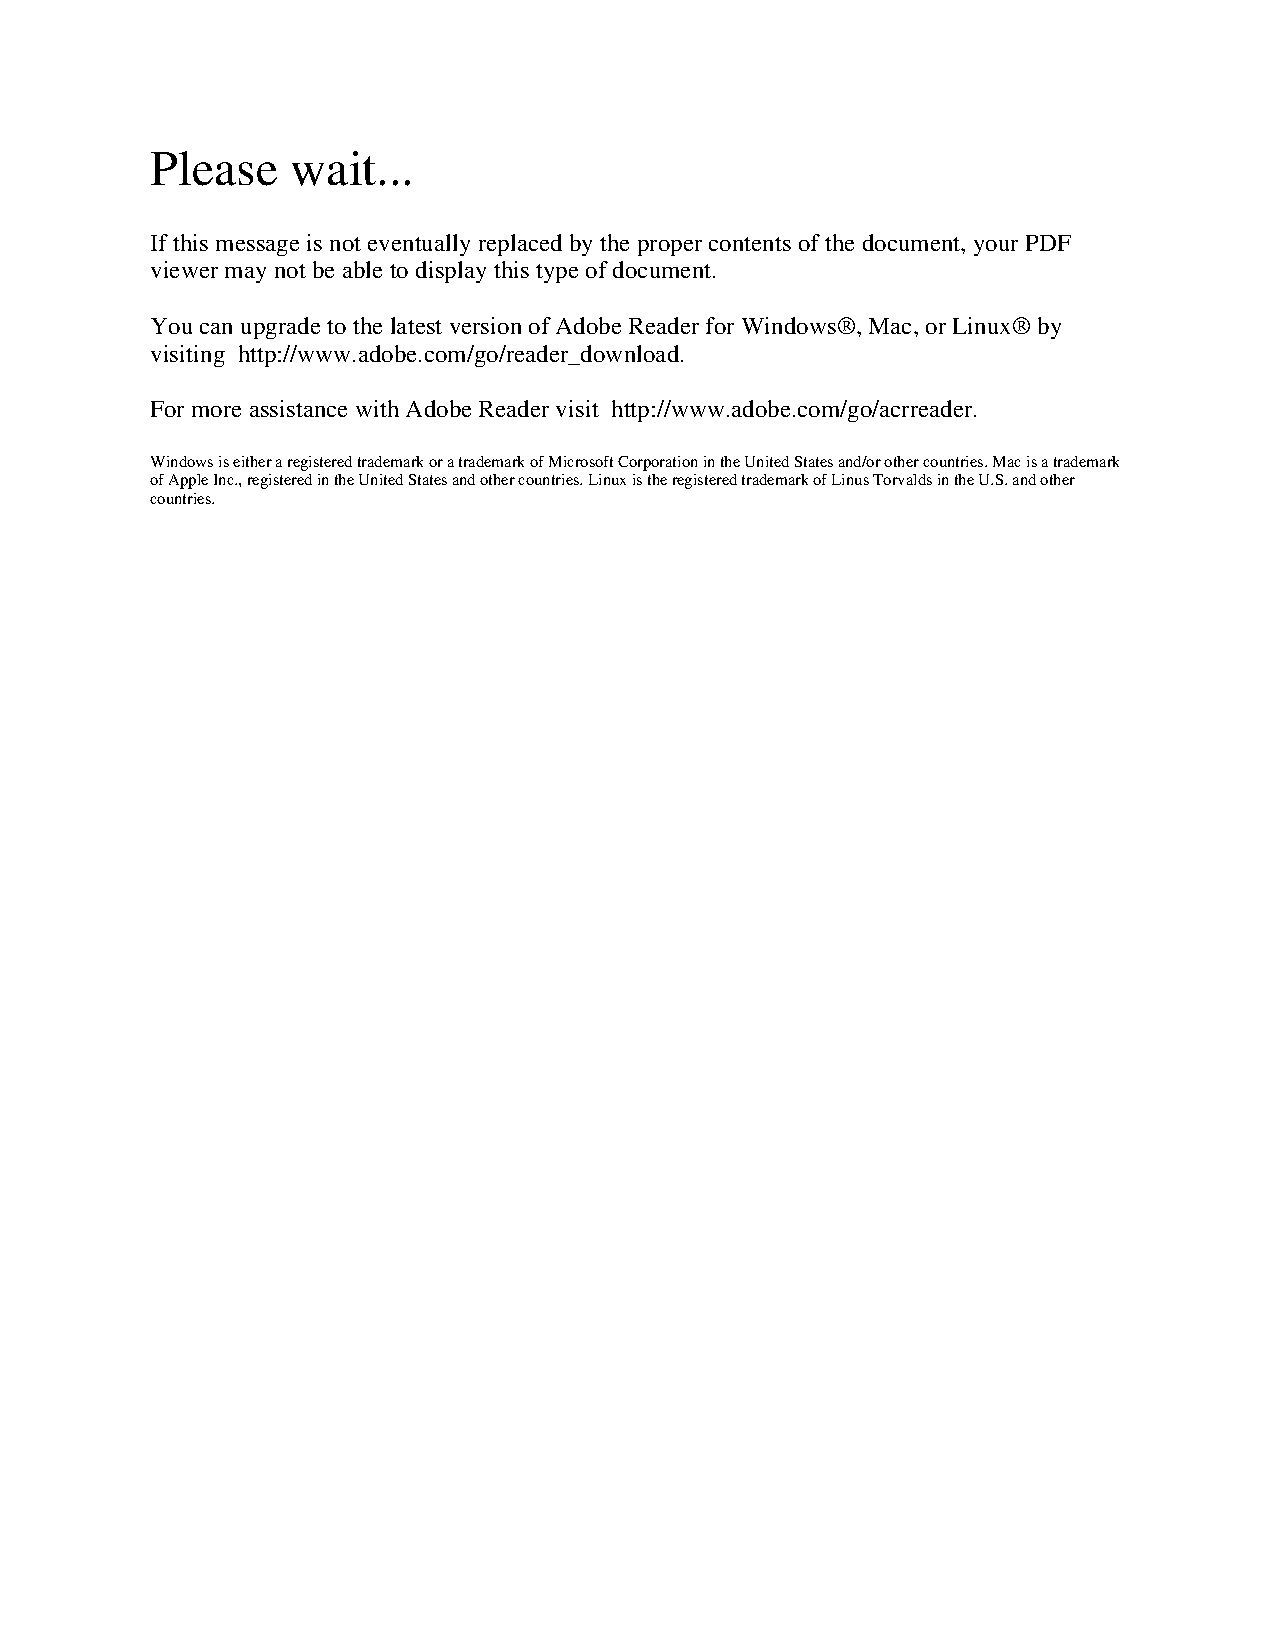
\includepdf[scale=1,pages=1]{confirmation/confirmation_en.pdf}
%---------------------------------------------------------------------------
\end{document}
%===========================================================================
